\documentclass[12pt]{article}

% double-spacing
\usepackage{setspace}
\doublespacing

%% line numbers
%% (turn on before submission)
%\usepackage{lineno}
%\linenumbers

% 1 inch margins
\usepackage[margin=1in]{geometry}

% text color
\usepackage{xcolor}

% bold symbols
\usepackage{bm}

% matrices
\usepackage{amsmath}

% images
\usepackage{graphicx}

% links
\usepackage{hyperref}

% remove section from figure number
%\usepackage{chngcntr}
%\counterwithout{figure}{section}

% bibliography
\usepackage[super]{natbib} % superscripts
\renewcommand{\refname}{} % empty title
\setcitestyle{citesep={,}} % comma separated

% highlight text that needs editing in red
\newcommand{\edit}[1]{{\color{red}{#1}}}
\newcommand{\add}[1]{{\color{red}{[... #1 ...]}}}

\begin{document}

\section*{Target Journal}

\textit{American Journal of Human Genetics}

\noindent\edit{Other ideas: \textit{PLoS Genetics}, \textit{Genetic Epidemiology}}  %, \textit{Nature Genetics}



\section*{Title}

% no more than 3 lines
% each line <= 54 characters (including spaces)
% convey conceptual significance of paper to broad readership

Adjusting for principal components can induce spurious 
associations in genome-wide association studies in admixed populations

\section*{Authors and Affiliations}

Kelsey E. Grinde,$^{1}$* % should I also list UW?
%Timothy A. Thornton,$^{2,3}$
%Alexander Reiner,
Brian L. Browning,$^{2}$ 
Sharon R. Browning$^{3}$

%% add Lisa, Alex, Tim if we use WHI data

\begin{enumerate}
\item Department of Mathematics, Statistics, and Computer Science, Macalester College, Saint Paul, MN, 55105, USA
\item Division of Medical Genetics, Department of Medicine, University of Washington, Seattle, WA, 98195, USA
\item Department of Biostatistics, University of Washington, Seattle, WA, 98195, USA
%\item \add{Regeneron}
\item[*] kgrinde@macalester.edu
\end{enumerate}

\edit{add Tim and Alex since using WHI data}


\newpage
\section*{Abstract}

% single paragraph
% <= 250 words
% convey conceptual advance and significance of work to broad readership
% brief background of question, description of results, brief summary of significance of findings
% do not cite any references

%% (from IGES submission)
%% currently 249 words
Principal component analysis (PCA) is widely used to control for population structure in genome-wide association studies (GWAS). It has been shown that the top principal components (PCs) typically reflect population structure, but deciding exactly how many PCs to include in GWAS regression models can be challenging. Often researchers will err on the side of including more PCs than may be actually necessary in order to ensure that population structure is fully captured. However, through both theoretical results and application to Women's Health Initiative SNP Health Association Resource genotype data and Trans-Omics for Precision Medicine whole genome sequence data for unrelated African American individuals from the Jackson Heart Study (JHS) and Chronic Obstructive Pulmonary Disease Genetic Epidemiology Study (COPDGene), we show that adjusting for extraneous PCs can actually induce spurious associations. In particular, spurious associations arise when PCs capture multiple local genomic features, such as regions of the genome with atypical linkage disequilibrium (LD) patterns, rather than genome-wide ancestry. We show that careful LD pruning prior to running PCA, using stricter thresholds than is often suggested in the literature, can resolve these issues, whereas excluding lists of high LD regions identified in previous studies does not. We also show that the rate of spurious associations can be appropriately controlled when we simply adjust for either the first PC or a model-based estimate of admixture proportions. Our work demonstrates that great care must be taken when using principal components to control for population structure in genome-wide association studies in admixed populations.


\newpage
\section{Introduction}

% succinct
% no subheadings
% present background info necessary to provide biological context for results


%% what is ancestral heterogeneity?
%Admixed populations such as African Americans and Hispanics/Latinos have historically been vastly underrepresented in genome-wide association studies (GWAS) \cite{need2009, bustamante2011, popejoy2016, morales2018, sirugo2019, martin2019}. 
Considerable variability in global ancestry---the genome-wide proportion of genetic material inherited from each ancestral population---has been observed in many studies of admixed populations such as African Americans and Hispanics/Latinos \citep{parra1998, tishkoff2009, bryc2010aa, bryc2010hl, conomos2016}.
It has been widely documented that heterogeneous global ancestry, as with other types of population structure, can lead to spurious associations in genome-wide association studies \citep{GenomicControl, eigenstrat, marchini2004, price2010}. 
In fact, some authors have even cited the ancestral heterogeneity of admixed populations, and the statistical challenges it poses, as one (among many) reason why these populations have been historically underrepresented in genome-wide association studies (GWAS) \citep{need2009, bustamante2011, popejoy2016, hindorff2018, manolio2019}.
%% why do we need to adjust for it?  (confounding)
Spurious associations can arise in GWAS in ancestrally heterogeneous populations when global ancestry confounds the association between genotypes and the phenotype of interest (Figure \ref{fig:confounding}). 
This confounding occurs when the genetic variant being tested differs in frequency across ancestral populations (i.e., global ancestry is associated with genotype) and global ancestry also has an effect on the phenotype via, for example, environmental factors or causal loci elsewhere in the genome that differ in frequency across ancestral groups.

%%% Figure 1: Confounding DAG %%%
\begin{figure}[h]
\center
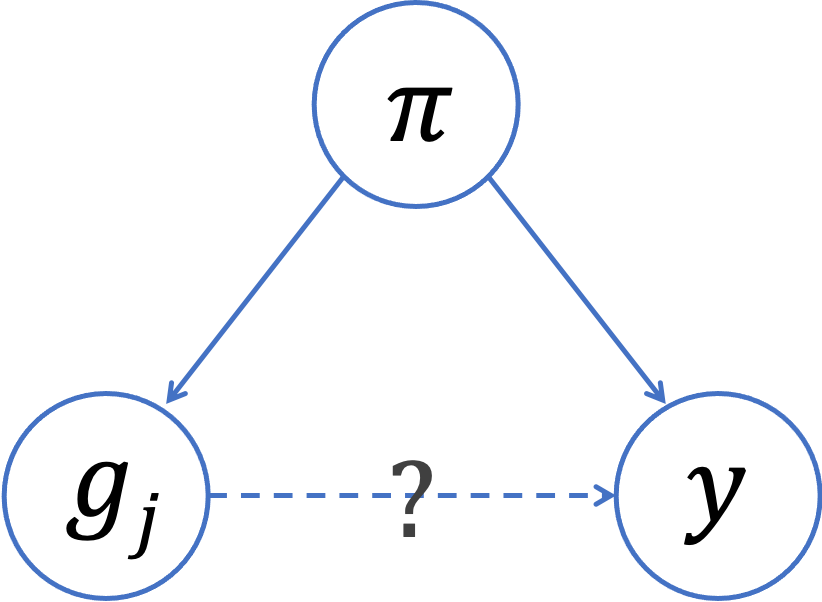
\includegraphics[width=0.4\textwidth]{figs/confounding}
\caption{Global ancestry ($\boldsymbol\pi$) confounds the association between the genotype at position $j$ ($\mathbf{g}_j$) and the phenotype of interest ($\mathbf{y}$) if ancestry is associated with both the genotype (e.g., the allele frequencies differ across the ancestral populations) and the phenotype (e.g., there are environmental or other factors that affect the phenotype and differ across the ancestral populations).}
\label{fig:confounding}
\end{figure}


%% how do we adjust
A number of methods for detecting and controlling for ancestral heterogeneity in genetic association studies have been proposed. 
Early approaches included restricting analyses to subsets of ancestrally homogeneous individuals \citep{lander1994}, performing a genome-wide correction for test statistic inflation due to ancestral heterogeneity via \textit{genomic control} \citep{GenomicControl}, and using family-based designs \citep{tdt}. 
More recently, approaches based on mixed models have been proposed \citep{yu2006, kang2010, yang2014}, using random effects to control for both close (e.g., due to family-based sampling) and distant (e.g., due to shared ancestry) relatedness across individuals.
When studies do not include closely related individuals, a simpler approach is to include inferred global ancestry as a fixed effect in marginal regression models \citep{eigenstrat, pritchard2000}. 
This fixed effects adjustment for global ancestry is used extensively throughout the literature, with global ancestry inferred using either model-based ancestry inference methods (e.g., \texttt{frappe} \citep{tang2005}, \texttt{STRUCTURE} \cite{structure}, \texttt{ADMIXTURE} \citep{admixture}, \texttt{RFMix} \citep{rfmix}) or principal component analysis (e.g., \texttt{EIGENSTRAT} \citep{eigenstrat}, \texttt{SNPRelate} \citep{snprelate}, \texttt{PC-AiR} \citep{conomos2015}).

% summarize model-based approaches (SKIP --- don't want to emphasize as much)
%Model-based approaches for global ancestry inference model the probability of observed genotypes given unobserved ancestry and allele frequencies in each ancestral population \citep{structure, tang2005, admixture, finestructure}. 
%Most often, these approaches are used to estimate global ancestry proportions, also known as \textit{admixture proportions}, the estimated proportion of genetic material inherited by each individual from each ancestral population. 
%Once estimated, these global ancestry proportions can then easily be included as covariates in GWAS models to adjust for ancestral heterogeneity.
%One of the challenges of using these model-based approaches to infer global ancestry is that the total number of ancestral populations usually needs to be pre-specified. 
%In addition, many of these model-based approaches are \textit{supervised}, requiring reference panel data from each ancestral population of interest to estimate allele frequencies.
%Furthermore, ancestry inference is typically conducted at a continental level (e.g., African versus European, rather than South European versus North European), so finer levels of population structure could be missed; recent efforts have considered global ancestry inference on a sub-continental scale \citep{finestructure, durand2014}.

%% overview of PCA 
Principal component analysis (PCA) is a widely-implemented unsupervised approach for inferring global ancestry that offers the advantages of not requiring reference panel data or pre-specification of the number of ancestral populations of interest.
It is also capable of capturing sub-continental structure \citep{novembre2008}. 
To infer global ancestry using PCA, we preform a singular value decomposition of the matrix of standardized genotypes (i.e., $\mathbf{X} = \mathbf{U}\mathbf{D}\mathbf{V}^\top$) or, equivalently, an eigenvalue decomposition of the genetic relationship matrix (i.e., $\mathbf{X}\mathbf{X}^\top = \mathbf{U}\mathbf{D}^2\mathbf{U}^\top$).
%where $\mathbf{X}$ is the $n \times m$ matrix of standardized gentoypes for $n$ individuals at $m$ single nucleotide variants (SNVs).
It has been shown that top eigenvectors, or \textit{principal components} (PCs), $\mathbf{u}_1, \mathbf{u}_2, \dots$ tend to reflect global ancestry \citep{patterson2006, mcvean2009}.
To adjust for ancestral heterogeneity in genome-wide association studies, we choose some number of PCs %(typically on the order of 1--10 \citep{abegaz2019}
to include as covariates in our GWAS regression models. 

%% issues & solutions: choosing P
Determining the number of PCs needed to capture global ancestry is non-trivial. 
Numerous techniques have been proposed, including formal significance tests based on Tracy-Widom theory \citep{patterson2006, eigenstrat}, examining inflation factors \citep{reed2015, conomos2016} and/or the proportion of variance explained by each PC \citep{raska2012, reed2015, conomos2016}, comparing PCs to self-reported race/ethnicity \citep{conomos2016}, and keeping PCs that are significantly associated with the trait \citep{reiner2012, daya2019}.
Typically, the number of PCs selected is on the order of one to ten \citep{abegaz2019}, but in practice it is not uncommon to see applications in which more many more PCs are used---more even than may actually be necessary to capture global ancestry. 
This could be due in part to work that has suggested that including higher-order PCs can provide the safeguard of removing ``virtually all stratification" \citep{mathieson2012} at the cost of perhaps only ``subtle" decreases in power \citep{liu2011}.
%using the same number of PCs as had been used  to prior work in distinct study populations to justify the choice of 10 PCs \citep{liu2012, reed2015}

%% issues & solutions: other atrifacts 
Another challenge that can arise in using PCA to adjust for ancestral heterogeneity involves ensuring that PCs actually reflect global ancestry and not some other features or artifacts of the data. 
Prior work has shown that PCs can capture relatedness across samples \citep{patterson2006, price2010, abdellaoui2013, conomos2015}, array artifacts or other data quality issues \citep{patterson2006, eigenstrat, price2010, weale2010}, and/or small regions of the genome with unusual patterns of linkage disequilibrium (LD) \citep{patterson2006, eigenstrat, wellcome2007, tian2008, price2008, price2010, weale2010, zou2010, laurie2010, abdellaoui2013, prive2020}. 
%\add{what happens if we adjust for PCs that capture LD instead? include here or save for discussion?}
To address this last issue, many authors have suggested running PCA on a reduced subset of variants after first performing \textit{LD pruning}, using a program such as \texttt{PLINK} \citep{plink} to remove variants that are in ``high" LD (e.g., pairwise-correlation $r^2 > 0.2$) with nearby variants  \citep{wellcome2007, fellay2007, novembre2008, yu2008, nelson2008, anderson2010, weale2010, laurie2010, abdellaoui2013, zhang2013, conomos2015, reed2015, galinsky2016, conomos2016, daya2019}, and/or excluding regions of the genome that are known to have extensive, long-ranging, or otherwise unusual patterns of LD \citep{wellcome2007,  fellay2007, novembre2008, price2008, anderson2010, weale2010, raska2012, conomos2016}. 
A list of these previously-identified high LD regions and references that recommend their exclusion are provided in Table \ref{tab:highLD}.
%after first removing regions of the genome that are known to have high or long-range LD (see Table \ref{tab:highLD}) \citep{wellcome2007,  fellay2007, novembre2008, price2008, anderson2010, weale2010, raska2012, conomos2016} and/or performing LD pruning (i.e., using a program such as \texttt{PLINK} \citep{plink} to remove variants that are in high LD) \citep{wellcome2007, fellay2007, novembre2008, yu2008, nelson2008, anderson2010, weale2010, laurie2010, abdellaoui2013, zhang2013, conomos2015, reed2015, galinsky2016, conomos2016, daya2019}. 


\begin{table}
\center
\begin{tabular}{crrl}
Chr & Start (bp) & End (bp) & References \\
\hline
1   & 48000000     & 52060567   &    \citep{anderson2010, price2008, weale2010} \\
2   & 85941853     & 100500000   &    \citep{anderson2010, price2008, weale2010} \\
2   & 129600000   & 140000000   &    \citep{price2008, novembre2008, weale2010, raska2012, conomos2016, prive2018} \\
2   & 182882739    & 190000000   &    \citep{anderson2010, price2008, weale2010} \\
3   & 47500000     & 50000000    &   \citep{anderson2010, price2008, weale2010}  \\
3   & 83500000     & 87000000    &   \citep{anderson2010, price2008, weale2010} \\
3   & 89000000     &   97500000   &    \citep{price2008, weale2010} \\
3   & 163100000    &   164900000   &    \citep{prive2018} \\
5   & 44000000     &   51500000    &   \citep{fellay2007, anderson2010, price2008, weale2010} \\
5   & 98000000     &  100500000   &    \citep{price2008, weale2010} \\
5   & 129000000    &   132000000   &    \citep{anderson2010, price2008, weale2010} \\
5   & 135500000    &   138500000   &   \citep{price2008, weale2010} \\
6   &  23800000     &   39000000   &    \citep{fellay2007, anderson2010, price2008, novembre2008, weale2010, raska2012, conomos2016, prive2018} \\
6   &  57000000     &   64000000   &    \citep{anderson2010, price2008, weale2010}  \\
6   & 140000000    &   142500000   &    \citep{anderson2010, price2008, weale2010}  \\
7   &  55000000     &   66193285   &    \citep{anderson2010, price2008, weale2010}  \\
8   &   6300000      &  13500000   &    \citep{fellay2007, anderson2010, price2008, novembre2008, tian2008, weale2010, raska2012, conomos2016, prive2018} \\
8   &  43000000    &    50000000   &    \citep{anderson2010, price2008, weale2010}  \\
8   & 112000000    &   115000000    &   \citep{anderson2010, price2008, weale2010} \\
10  &  37000000    &    43000000   &    \citep{anderson2010, price2008, weale2010}  \\
11   & 45000000    &    57000000   &    \citep{fellay2007, price2008, weale2010} \\
11   & 87500000    &    90500000   &    \citep{anderson2010, price2008, weale2010}  \\
12   & 33000000    &    40000000   &    \citep{anderson2010, price2008, weale2010} \\
12   & 109500000   &    112021663   &    \citep{price2008, weale2010} \\
14   & 46600000    &    47500000   &    \citep{prive2018} \\
17   & 37800000    &    42000000    &   \citep{novembre2008, conomos2016} \\
20   & 32000000   &     34500000    &   \citep{anderson2010, price2008, weale2010}  \\
\end{tabular}
\caption{Regions of the genome with high, long-range, or otherwise unusual patterns of linkage disequilibrium (LD) that are often recommended for exclusion prior to running PCA. This list of regions was generated on the basis of an extensive literature review. Start and end physical (base pair) positions are provided with respect to genome build 36. Also available for download (in builds 36, 37, or 38) at \href{github.com/kegrinde/PCA}{https://github.com/kegrinde/PCA/}.}
\label{tab:highLD}
\end{table}


%% motivate  our paper
The above-cited suggestions regarding LD pruning and filtering are not universally implemented and the downstream implications of adjusting for PCs that capture features other than global ancestry are not fully understood.
Furthermore, much of this prior work was conducted in populations of European ancestry, so recommendations on how best to implement principal component-based adjustment for ancestral heterogeneity in admixed populations are lacking. 
% outline rest of paper
In this paper, we investigate the impact of LD filtering and pruning choices, as well as choices of the number of principal components to include in analyses, on genome-wide association studies in admixed populations.
We show that principal components may capture local genomic features, unless careful pre-processing is performed prior to analysis.
We also conduct simulation studies and provide analytic results to show that including too many PCs can actually induce spurious associations in GWAS, particularly when those extraneous PCs capture local genomic features rather than genome-wide ancestry.
To conclude, we provide suggestions regarding best practice for appropriately controlling for ancestral heterogeneity in genome-wide association studies in admixed populations.



\section{Material and Methods}

% provide sufficient detail so readers can understand how experiments were performed and procedures can be repeated
% describe any statistical methods employed in study

\subsection{Data and Quality Control}

Our analyses focus on genotype and sequence data from three samples of unrelated African American individuals.
In particular, we consider genotype data from the Women's Health Initiative SNP Health Association Resource (WHI SHARe), as well as whole genome sequencing data from two contributing studies to the Trans-Omics for Precision Medicine (TOPMed) Whole Genome Sequencing Project: the Jackson Heart Study (JHS) and the Genetic Epidemiology of Chronic Obstructive Pulmonary Disease Study (COPDGene).
We performed quality control (QC) and identified subsets of unrelated African American individuals prior to running any further analyses.

\subsubsection{WHI SHARe Genotype Data}

The Women's Health Initiative (WHI) is a long-term study of the health of women in the United States.
In total, 161,808 postmenopausal women aged 50--79 years old were recruited to participate in this study.
Additional details on study design and cohort characteristics can be found elsewhere \cite{whi}.
Included in the WHI study are 12,151 self-identified African American women who consented to genetic research, a subsample of which were selected for genotyping using the Affymetrix Genome-Wide Human SNP Array 6.0.
This array contains 906,000 single nucleotide polymorphisms (SNPs) and more than 946,000 probes for the detection of copy number variants; in these analyses, we focus only on the SNPs.

The genotype data were processed for quality control, including call rate, concordance rates for blinded and unblinded duplicates, and sex discrepancy, leaving 871,309 unflagged SNPs with a genotyping rate of 99.8\% and 8,421 African American women \cite{reiner2012}.
We additionally used the iterative procedure suggested by Conomos et al. \cite{conomos2016related} to identify a subset of 8,064 mutually unrelated individuals, using a kinship threshold of 0.044 (i.e., excluding first, second, and third degree relatives).

\subsubsection{TOPMed Whole Genome Sequence Data}

The Trans-Omics for Precision Medicine (TOPMed) Whole Genome Sequencing Project is an ongoing project sponsored by the National Heart, Lung, and Blood Institute (NHLBI).
The goal of this project is to collect and analyze whole-genome sequences, other omics data, and rich phenotypic information for over 100,000 individuals from diverse backgrounds. 
Data are periodically released on dbGaP for analysis by the broader scientific community. 
Our analysis uses data from \textit{freeze 4}, released in 2017, and \textit{freeze 5b}, released in 2018.
These two freezes include samples from a large number of contributing studies.
We focus on two such studies: the Jackson Heart Study (JHS) (accession number: phs000964) and the Genetic Epidemiology of Chronic Obstructive Pulmonary Disease Study (COPDGene) (accession number: phs000951).
In total, the freeze 4 JHS dataset includes 3,406 African American individuals and the freeze 5b COPDGene dataset includes 8,742 African American and European American individuals.
% sequencing
For TOPMed freezes 4 and 5b, high coverage ($\approx$ 30X) whole genome sequencing was performed by several sequencing centers.
Variant discovery and genotype calling was performed by the TOPMed Informatics Resources Center (IRC) using the \texttt{GotCloud} pipeline \citep{jun2015}.

% QC
Quality control (QC) was performed by the sequencing centers, IRC, and TOPMed Data Coordinating Center, and only those samples and variants that passed these stages of QC are included in the Variant Call Format (VCF) files downloaded from dbGaP.
% references
Details on TOPMed sequencing and QC methods are available in Taliun et al. \citep{taliun2021} and on the TOPMed website: \href{https://topmed.nhlbi.nih.gov/data-sets}{https://topmed.nhlbi.nih.gov/data-sets}.
%% filters applied universally
Prior to genetic ancestry inference, we performed two additional stages of variant- and sample-level filtering.
% bcftools filters from Joe
We used \texttt{bcftools} \citep{bcftools} to remove indels and otherwise restrict our analyses to biallelic single nucleotide variants (SNVs). 
% relatives 
Finally, we used the \href{https://github.com/UW-GAC/analysis_pipeline}{University of Washington Genetic Analysis Center TOPMed analysis pipeline} to restrict our analyses to a subset of mutually unrelated individuals (kinship threshold = 0.044)\citep{conomos2016related} .
%\edit{Will this confuse people? Is saying we used the TOPMed pipeline enough? Perhaps skip?:} Note that this procedure of identifying related individuals involves an initial step of LD pruning and filtering, as recommend by the TOPMed Analysis Pipeline.
After filtering, 2,777 and 8,476 samples and 77,136,850 and 135,522,041 variants remained in JHS and COPDGene, respectively.


\subsection{Genetic Ancestry Inference}

We consider two approaches to inferring genetic ancestry in these admixed samples: model-based approaches and principal component analysis.

\subsubsection{Model-Based Approaches}

In WHI SHARe African Americans, we inferred both local and global genetic ancestry using model-based ancestry inference techniques. 
Local ancestry inference was performed using \texttt{RFMix} \citep{rfmix} and a reference panel including individuals of European and African decent from the International HapMap Project (HapMap) \citep{hapmap}: see Grinde et al. \cite{steam} for more details.
We then calculated global ancestry proportions via the genome-wide average local ancestry $\hat\pi_{ik} = \frac{1}{2m}\sum_{j=1}^m a_{ijk},$ where $a_{ijk}$ is the inferred number of alleles (0, 1, or 2) inherited by individual $i$ at variant $j$ from ancestral population $k$.
We also compared these \texttt{RFMix}-based global ancestry estimates to results from supervised and unsupervised \texttt{ADMIXTURE}  \citep{admixture} analyses with two ancestral populations ($K = 2$).
The supervised analysis used the same HapMap reference panel as was used to infer local ancestry using \texttt{RFMix}.
% supervised = same Hap
All three sets of admixture proportions were highly correlated (pairwise Pearson correlation $>$ 0.998), so we proceed with using only the \texttt{RFMix}-based admixture proportion estimates for the remainder of our analyses.

In TOPMed JHS and COPDGene samples, we inferred global ancestry via unsupervised \texttt{ADMIXTURE} analyses with both two and three ancestral populations (i.e., $K = 2$ and $K = 3$). 
% did not do supervised or RFMix because more time-intensive
We also used these inferred global ancestry proportions to identify subsets of admixed individuals.
In particular, the COPDGene study includes both African American and European American individuals, but  self-identified race/ethnicity information was not available from dbGaP.
Instead, we used inferred admixture proportions to identify and restrict our attention to individuals with at least 29.5\% African ancestry.
% although these analyses were unsupervised, we inferred which ancestral population corresonded to African ancestry based on observed ancestry proportions
The choice of threshold follows from the results reported by Parker et al. \cite{parker2014}, showing that the self-identifed African American individuals in the COPDGene study have inferred proportions of African ancestry ranging from 29.5\% and above.
(Note that we are not suggesting that this same threshold be universally applied to identify African American individuals in other samples.)
After filtering, 2,676 individuals remain. 
In addition, although JHS is known to focus on African Americans, we did identify some individuals inferred to have 100\% European ancestry in that sample.
These individuals were excluded from further analyses, leaving a total of 1,888 admixed samples. 


\subsubsection{Principal Component Analysis}

%% PCA in WHI
We ran PCA on the WHI SHARe genotype data using \texttt{SNPRelate} \citep{snprelate}. 
First, we applied PCA to the set of all 551,025 SNPs with available genotypes.
%We refer to these PCs as the \textit{naively generated PCs}.
We then applied PCA to subsets of SNPs based on the following pre-processing criteria: excluding SNPs falling into regions of the genome that have been cited in the literature as potentially problematic for PCA (Table \ref{tab:highLD}), LD pruning with an $r^2$ threshold of 0.1 and window size of 0.5 mega basepairs (Mb), or both literature-based exclusions and LD pruning.
LD pruning and literature-based filters were implemented using the \texttt{SNPRelate} package.
Table \ref{tab:preprocessN} summarizes the number of SNPs remaining after each set of pre-processing steps.
After running PCA on these different sets of variants, we also used \texttt{SNPRelate} to assess the contribution of each SNP to each principal component by calculating the SNP loadings and the correlation between PCs and genotypes.

\begin{table}
\small
\begin{tabular}{|l|rrr|}
\hline
 & WHI SHARe & TOPMed JHS & TOPMed COPDGene \\
\hline
Neither Exclude nor Prune & 551,025 & 14,117,957 & 13,959,378 \\
Exclude High LD Regions (Table \ref{tab:highLD}) & 536,668 & 13,723,944 & 13,575,038  \\
LD Prune ($r^2 < 0.1$, 0.5 Mb windows) & 49,723  &  245,003 & 251,040  \\
Both Exclude and Prune & 48,794 & 239,425  & 245,378  \\
\hline
\end{tabular}
\caption{Number of autosomal variants remaining after different combinations of pre-processing steps were applied prior to running PCA. Note that TOPMed analyses additionally applied a filter to keep only those variants with minor allele frequency greater than 0.01.} 
\label{tab:preprocessN}
\end{table}

%% PCA in TOPMed
In TOPMed JHS and COPDGene samples, we used the University of Washington Genetic Analysis Center (UW GAC) TOPMed analysis pipeline to implement pre-processing, run principal component analysis, and calculate and visualize the contribution of individual variants to each PC. 
Similar to WHI SHARe, we applied PCA to various subsets of variants based on different pre-processing criteria, including a naive analysis with no prior LD-based pruning or filtering, an analysis after excluding the regions listed in Table \ref{tab:highLD}, an analysis after LD pruning with an $r^2$ threshold of 0.1, and an analysis after both LD-based pruning and filtering.
Following the recommendations of Kirk \citep{JKdissertation} and the UW GAC pipeline documentation, we also removed variants with a minor allele frequency lower than 0.01 in all cases.
Note that the UW GAC pipeline does provide the option to exclude some of the regions listed in Table \ref{tab:highLD} (the \textit{LCT} gene on chromosome 2, the HLA region on chromosome 6, and the locations of large inversions on chromosomes 8 and 17), but we customized the pipeline code slightly to add the other regions identified in our literature review. 
See Table \ref{tab:preprocessN} for the number of variants included in each analysis.

%\begin{table}
%\begin{tabular}{ccccc}
%name & chrom & start.base  & end.base  & comment \\
%2q21    &  2  &  129125957 & 139525961       &  LCT \\
%HLA      &    6 &   24091793  & 38924246 & includes MHC \\
%8p23  &        8   &  6755071 &  13598120 &   inversion \\
%17q21.31 &    17  &  42394456 & 46567318   &  inversion \\
%\end{tabular}
%\caption{TOPMed hg38 high corr regions}
%\end{table}



\subsection{Simulation Study}

To explore the impact of adjusting for principal components that capture local genomic features, we conducted a simulation study using genotype data and simulated traits in the WHI SHARe African American sample.

\subsubsection{Trait Simulation}

Traits were simulated for each individual $i = 1, \dots, 8064$ such that they depended only on the genotype $g_{ij}$ at a single causal variant with effect size $\beta_j$: $$y_i = \beta_j g_{ij} + \epsilon_i, \ \epsilon_i \stackrel{iid}{\sim} N(0, 1).$$
We considered seven choices of effect sizes ($\beta_j = 0, 0.25, 0.5, 1, 2, 4, 8$) and 473 choices for the position $j$ of the causal variant, varying the position of this causal variant across all 22 autosomes.

To choose the location of these causal variants, we first estimated the difference in ancestral allele frequencies for each variant using the observed allele frequencies in our HapMap reference panel (which included samples from the CEU (Utah residents with Northern and Western European ancestry) and YRI (Yoruba in Ibadan, Nigeria)  populations: see Grinde et al. \citep{steam} for more details).
We also considered the SNP loadings %(i.e., the contribution of each SNP to each PC \add{\cite{136}}) 
for the set of PCs that were generated without any prior LD-based filtering or pruning.
%Based on these calculations, we selected 473 variants with positions spread across the genome, high or low SNP loadings, and large or small ancestral allele frequency differences.
We identified the 10 variants on each chromosome with the highest absolute SNP loading for each of the first four PCs. 
In total, 373 unique variants were selected according to 	this procedure. 
For comparison, we also selected 100 variants across the autosomes with low SNP loadings ($|\text{loading}| < 0.0008$) for all of the first four PCs.
Among these 100 variants, 85 were selected such that they had different allele frequencies in the African and European ancestral populations ($|\hat{p}_{CEU} - \hat{p}_{YRI}| > 0.6$), and 15 were selected that had similar allele frequencies in the two ancestral populations ($|\hat{p}_{CEU} - \hat{p}_{YRI}| < 0.005$).


\subsubsection{GWAS Models}

For each simulated trait, we ran genome-wide association studies using models of the general form
$$E[y_i \mid g_{ij}, \mathbf{w}_i] = \alpha + \beta_j g_{ij} + \boldsymbol\gamma \mathbf{w}_i,$$
where $y_i$ is the simulated quantitative trait, $g_{ij}$ is the genotype at position $j$,  and $\mathbf{w}_i$ is a vector of additional covariates.
Note that we quantify genotype $g_{ij}$ by the number of copies---0, 1, or, 2---of some pre-specified allele (e.g., the minor allele) carried by individual $i$ at position $j$.
We fit these models at every position $j = 1, \dots, m$ across the genome and test for association between the trait and genotype by testing the null hypothesis $H_0: \beta_j = 0$ using a traditional Wald test.

In particular, we consider four models: a model making no adjustment for ancestral heterogeneity (i.e., $\mathbf{w}_i = \emptyset$), a model adjusting for model-based admixture proportions ($\mathbf{w}_i = \hat\pi_i$), a model adjusting for the first principal component ($\mathbf{w}_i = u_{1i}$), and a model adjusting for the first four principal components ($\mathbf{w}_i = \begin{bmatrix} u_{1i} & u_{2i} & u_{3i} & u_{4i} \end{bmatrix}$). 
For the models adjusting for principal components, we consider four sets of PCs based on different pre-processing criteria: \textit{none} (no prior LD-based exclusions or pruning), \textit{exclusions only} (excluding regions from Table \ref{tab:highLD} but no LD pruning), \textit{pruning only} (LD pruning with $r^2 < 0.1$ and a window size of 0.5 Mb, but not excluding regions from Table \ref{tab:highLD}), and \textit{both} (both Table \ref{tab:highLD} exclusions and LD pruning).

\subsubsection{Spurious Associations}

To evaluate these ancestral heterogeneity adjustment approaches, we compared the number of spurious associations that appeared when we used each model.
We quantified spurious associations by counting the number of chromosomes, not including the chromosome on which the causal variant was located, with at least one variant reaching genome-wide significance.
For all models, the genome-wide significance threshold was set to the $p = 5.0 \times 10^{-8}$ threshold that is used extensively throughout the GWAS literature \cite{peer2008, jannot2015}.


\subsection{Data and Software Availability}

WHI SHARe genotype data and TOPMed whole genome sequence data are available for analysis upon request and application. Visit study sites and dbGaP for more information.
All software packages used throughout this paper are freely available online: 

%Data: 
%\begin{itemize}
%\item WHI Data: \edit{TBD}
%\item TOPMed Sequence Data: \href{https://www.ncbi.nlm.nih.gov/gap/}{https://www.ncbi.nlm.nih.gov/gap/}
%\end{itemize}

\begin{itemize}
\item bcftools \citep{bcftools} (quality control): \href{https://samtools.github.io/bcftools/}{https://samtools.github.io/bcftools/}
%\item Beagle (phasing and imputation): 
\item RFMix \citep{rfmix} (local ancestry inference):  \href{https://sites.google.com/site/rfmixlocalancestryinference/}{https://sites.google.com/site/rfmixlocalancestryinference/}
\item ADMIXTURE \citep{admixture} (global ancestry inference): \href{https://dalexander.github.io/admixture/}{https://dalexander.github.io/admixture/}
\item PCRelate \citep{conomos2016related} and PC-AiR \citep{conomos2015}
 (identifying unrelated individuals): \href{https://rdrr.io/bioc/GENESIS/}{https://rdrr.io/bioc/GENESIS/}
\item SNPRelate \citep{snprelate} (LD pruning, PCA, and PCA-related diagnostics): \\ \href{https://www.bioconductor.org/packages/release/bioc/html/SNPRelate.html}{https://www.bioconductor.org/packages/release/bioc/html/SNPRelate.html} 
\item PLINK \citep{plink} (GWAS): \href{https://zzz.bwh.harvard.edu/plink/}{https://zzz.bwh.harvard.edu/plink/}
\item TOPMed Analysis Pipeline (identifying unrelated individuals, LD pruning, PCA,  PCA-related diagnostics, and association studies in whole genome sequence data): \\ \href{https://github.com/UW-GAC/analysis_pipeline}{https://github.com/UW-GAC/analysis\_pipeline}
\item R (analyzing and visualizing results): \href{https://cran.r-project.org/}{https://cran.r-project.org/}
\end{itemize}

Other resources pertaining to this paper, including download-able lists of the high LD regions in Table \ref{tab:highLD} in various builds, can be found on the lead author's GitHub page: \href{https://github.com/kegrinde/PCA}{https://github.com/kegrinde/PCA}.



%old outline: 
%
%\begin{itemize}
%\item TOPMed data
	%\begin{itemize}
	%\item what is TOPMed
	%\item which studies did we focus on
	%\item how accessed
	%\item who's in it
	%\item freeze 4 sequencing methods (JHS)
	%\item freeze 5b methods (COPDGene)
	%\item TOPMed QC
	%\end{itemize}
%\item filtering
%	\begin{itemize}
	%\item basic SNP filters --> moved to TOPMed section
	%\item rare variants \add{move this to QC step?}; \add{citations}
	%\item missing rates \add{STILL NEED TO IMPLEMENT THIS!!}
	%\item relatives; \add{citations}
	%\item non-admixed individuals
	%\item LD pruning/filtering
	%\end{itemize}
%\item inferring ancestry using PCA
	%\begin{itemize}
	%\item software
	%\item types of pruning/filtering considered --> move to filtering
	%\item plots we look at (loadings, screeplots, parallel coordinates, etc.)
	%\end{itemize}
%\item inferring ancestry using ADMIXTURE --- skip since already mentioned in QC
	%\begin{itemize}
	%\item motivation for comparison
	%\item recommended pruning/filtering
	%\end{itemize}
%\item simulation study
%	\begin{itemize}
%	\item traits
%	\item models
%	\item evaluation
%	\end{itemize}
%\item software and data availability
	%\begin{itemize}
	%\item dbgap
	%\item github
	%\end{itemize}
%\end{itemize}


%\subsection{Old Methods}

%\textbf{QC for JHS} (dbgap accession phs000964):
%
%\begin{itemize}
%\item filtering
	%\begin{itemize}
	%\item bi-allelic SNPs
	%\item minor allele count at least 1
	%\item pass variant filters (in VCFs that were downloaded from dbgap): overlaps with SNP, overlaps with indel, overlaps with VNTR, failed SVM filter, high (3/5\% or more) mendelian or duplicate genotype discordance, excess heterozygosity with HWE p-value < 1e-6
	%\end{itemize}
%\item merge the two subsets (cg1 and cg3)
%\item convert from VCF to GDS
%\item remove close relatives
	%\begin{itemize}
	%\item run king (LD r threshold: 0.32, LD window size: 10, MAF threshold: 0.01, exclude PCA corr: TRUE, build: hg19)
	%\item run PC-AiR 
	%\item run PCRelate 
	%\item run PC-AiR again
	%\end{itemize}
%\item find African Americans
	%\begin{itemize}
	%\item run stricter LD pruning (MAF  = 0.01, window size = 0.5, rsq = 0.01, regions = TRUE, build 37)
		%\begin{itemize}
		%\item List of regions stored here: \verb"/projects/browning/brwnlab/kelsey/spurious_assoc/highLD_regions/" (see below)
		%\end{itemize}
	%\item convert GDS to BED
	%\item run ADMIXTURE (K = 2 and K = 3)
	%\item plot proportions
	%\item exclude 40 people inferred to be 100\% European; left with 1888
	%\end{itemize}
%\end{itemize}

%\textbf{QC for COPDGene} (phs000951):
%
%\begin{itemize}
%\item filtering
%	\begin{itemize}
%	\item bi-allelic SNPs
%	\item minor allele count at least 1
%	\item pass filtering (from GDS annotation info, I inferred this to include: variant located in centromeric region, variant failed SVM filter, mendelian or duplicate genotype discordance is high (3/5\% or more), excess heterozygosity in chrX in males, excess heterozygosity with HWE p-value < 1e-6)
%	\end{itemize}
%item convert from VCF to GDS
%\item remove close relatives
%	\begin{itemize}
%	\item run king (LD r threshod = 0.32, LD window size = 10, MAF threshodl = 0.01, exclude PCA corr = TRUE, build = hg38); regions =         see table below
%	\item run PCAiR
%	\item run PCRelate
%	\item run PCAiR again
%	\end{itemize}
%\item find African Americans
%	\begin{itemize}
%	\item run stricter LD pruning (exclude PCA corr regions = TRUE, build = hg38, LD R threshold = 0.1, LD window size = 10, MAF threshold = 0.01); regions = \verb"/projects/browning/brwnlab/kelsey/spurious_assoc/highLD_regions/" (see below)
%	\item convert from GDS to PLINK
%	\item run ADMIXTURE with K = 2 and K = 3
%	\item plot proportions and use cut-off of 30\% to identify (and then remove) Europeans : Parker et al. 2014 "Admixture mapping identifies a quantitative trait locus associated with..." \verb"https://www.ncbi.nlm.nih.gov/pmc/articles/PMC4190160/" (reduced from 8406 to 2676)
%	\end{itemize}
%\end{itemize}

%\begin{table}
%\begin{tabular}{ccccc}
%name & chrom & start.base  & end.base  & comment \\
%2q21    &  2  &  129883530 & 140283530       &  LCT \\
%HLA      &    6 &   24092021  & 38892022 & includes MHC \\
%8p23  &        8   &  6612592 &  13455629 &   inversion \\
%17q21.31 &    17  &  40546474 & 44644684   &  inversion \\
%\end{tabular}
%\caption{TOPMed hg19 high corr regions}
%\end{table}

%\begin{table}
%\begin{tabular}{ccccc}
%name & chrom & start.base  & end.base  & comment \\
%2q21    &  2  &  129125957 & 139525961       &  LCT \\
%HLA      &    6 &   24091793  & 38924246 & includes MHC \\
%8p23  &        8   &  6755071 &  13598120 &   inversion \\
%17q21.31 &    17  &  42394456 & 46567318   &  inversion \\
%\end{tabular}
%\caption{TOPMed hg38 high corr regions}
%\end{table}

%\begin{itemize}
%\item what filtering was performed, and how many variants left after filtering
%	\begin{itemize}
%	\item JHS, ADMIXTURE: see above
%	\item JHS, PCA: exclude regions (TRUE/FALSE), r-squared (1, 0.1, 0.2, 0.05), window size (0, 0.5, 10), and MAF (0, 0.01) 
%		\begin{itemize}
%		\item no filtering: FALSE-1-0-0
%		\item MAF filtering: FALSE-1-0-0.01
%		\item exclude but no prune: TRUE-1-0-0.01
%		\item prune but no exclude: FALSE-0.1-0.5-0.01 and FALSE-0.1-10-0.01 and FALSE-0.2-0.5-0.01 and FALSE-0.05-0.5-0.01
%		\item prune and exclude: TRUE-0.1-0.5-0.01 and TRUE-0.1-10-0.01 and TRUE-0.2-0.5-0.01 and TRUE-0.05-0.5-0.01
%		\end{itemize}
%	\item COPD, ADMIXTURE: see above
%	\item COPD, PCA: exclude regions (TRUE/FALSE), r-squared (1, 0.1, 0.2, 0.05), window size (0, 0.5, 10), MAF (0, 0.01)
%		\begin{itemize}
%		\item no filtering: FALSE-1-0-0
%		\item MAF filtering: FALSE-1-0-0.01
%		\item exclude but no prune: TRUE-1-0-0.01
%		\item prune but no exclude: FALSE-0.1-0.5-0.01, FALSE-0.1-10-0.01, FALSE-0.2-0.5-0.01, FALSE-0.05-0.5-0.01
%		\item prune and exclude: TRUE-0.1-0.5-0.01, TRUE-0.1-10-0.01, TRUE-0.05-0.5-0.01, TRUE-0.2-0.5-0.01
%		\end{itemize}	
%	\item COPD, also ran SNPRelate on Europeans with different levels of filtering (FALSE-0.1-0.5-0.01, FALSE-0.2-0.5-0.01, FALSE-1-0-0.01, FALSE-1-0-0, TRUE-0.1-0.5-0.01, TRUE-0.2-0.5-0.01, TRUE-1-0-0.01)
%	\end{itemize}
%\end{itemize}


%\subsection{Simulation Study to Investigate Rates of Spurious Associations}
%
%We implement a simulation study to explore the impact of different variant-level filtering choices, particularly with respect to linkage disequlibrium, on rates of spurious associations in genome-wide association studies using models that adjust for ancestral heterogeneity using principal components.
%
%\subsubsection{Simulated Traits}
%
%\add{
%\begin{itemize}
%\item find loading peaks from "naive" approach
%\item simulate trait that is beta * x + rnorm(0, 1), where beta = 1 or 2 and x = genotype at one of the peaks
%\end{itemize}
%}

%\subsubsection{GWAS Models}
%
%To perform genome-wide association studies in samples of unrelated admixed individuals, we use marginal regression models, regressing the trait of interest on the genotype at each position across the genome. 
%At a given position $j$, we quantify genotype $g_{ij}$ as the number of copies (0, 1, or 2) of some pre-specified allele (e.g., the minor allele) carried by individual $i$ at that position. 
%Considering a quantitative trait $y_i$, we fit one linear regression model at each position ($j = 1, \dots, m$): $$E[y_i \mid g_{ij}, \mathbf{z}_i] = \beta_0 + \beta_j g_{ij} + \boldsymbol{\beta}_z \mathbf{z}_i,$$ where $\mathbf{z}_i$ is a vector of additional covariates (e.g., potential confounding variables) that we want to include in the model.
%%This linear regression model can be replaced with a logistic regression model in the case of a binary trait (e.g., disease status).
%We test for an association between the trait and genotype by testing the null hypothesis $H_0: \beta_j = 0$ at each position $j = 1, \dots, m$.
%
%
%To adjust for ancestral heterogeneity, we include inferred global ancestry in the vector $\mathbf{z}_i$ of potential confounders in our regression models. We infer global ancestry using one of two techniques: model-based global ancestry inference of principal component analysis. 
%\add{describe which models we compare}
%
%\add{
%\begin{itemize}
%\item for each of 188*2 simulated phenotypes
%\item for each set of PCs
%\item including 1, 4, or 10 PCs
%\end{itemize}
%}

%% UPDATE: skipping details of model-based GAI
%\subsubsection{Model-based global ancestry inference}
%
%Various model-based approaches have been developed for estimating global ancestry proportions in admixed populations.
%We represent global ancestry via the vector $\boldsymbol{\pi}_i = \begin{pmatrix} \pi_{i1} & \dots & \pi_{iK} \end{pmatrix}^\top$, where $\pi_{ik}$ denotes the genome-wide proportion of genetic material inherited by individual $i$ from ancestral population $k$ and $\sum_{k=1}^K \pi_{ik} = 1$. 
%Note that the total number of ancestral populations, $K$, typically must be pre-specified, and the definition of global ancestry is typically restricted to the autosomes.
%Admixture proportions can be estimated directly using a program such as \texttt{ADMIXTURE} \citep{admixture}, or by calculating the genome-wide average local ancestry (i.e., $\hat\pi_{ik} = \frac{1}{2m} \sum_{j=1}^m a_{ijk}$), where local ancestry $a_{ijk}$---the number of alleles (0, 1, or 2) inherited by individual $i$ from ancestral population $k$ at position $j$---was first inferred using a program such as \texttt{RFMix} \citep{rfmix}.
%To adjust for ancestral heterogeneity, we include $K-1$ of these estimated admixture proportions as covariates in our GWAS regression models: $$E[y_i \mid g_{ij}, \hat{\boldsymbol\pi}_i] = \beta_0 + \beta_j g_{ij} + \beta_{\pi, 1} \hat\pi_{i,1} + \dots + \beta_{\pi, K-1} \hat\pi_{i, K-1}.$$
%
%Many model-based global ancestry inference programs are supervised, requiring data from individuals from each ancestral population of interest to form a reference panel. However, some approaches such as \texttt{ADMIXTURE} can also be run without a reference panel.

%% UPDATE: moved most of this to intro
%\subsubsection{Principal component analysis}
%
%Principal component analysis (PCA) is an unsupervised dimension-reduction technique that is widely used for inferring population structure in genetic studies, with a number of software programs available for running PCA on genotype or sequence data (e.g., \texttt{EIGENSTRAT} \citep{eigenstrat}, \texttt{SNPRelate} \citep{snprelate}, \texttt{PC-Air} \citep{conomos2015}).
%To run PCA, we perform a singular value decomposition of the matrix of standardized genotypes (i.e., $\mathbf{X} = \mathbf{UDV}^\top$) or, equivalently, an eigenvalue decomposition of the genetic relationship matrix (i.e., $\mathbf{XX}^\top = \mathbf{UD}^2\mathbf{U}^\top$). 
%The top principal components ($\mathbf{u}_1, \mathbf{u}_2, \dots$) typically capture global ancestry \citep{patterson2006, mcvean2009}. 
%To adjust for ancestral heterogeneity, we choose some number of principal components, $P$, needed to capture global ancestry (typically $1 \le P << n$) and include those PCs as covariates in our GWAS regression models: $$E[y_i \mid g_{ij}, u_{i1}, \dots, u_{iP}] = \beta_0 + \beta_j g_{ij} + \beta_{u 1} u_{i1} + \dots + \beta_{u P} u_{i P}.$$
%A number of techniques have been proposed for selecting the number of PCs, $P$, including formal significance tests based on Tracy-Widom theory \citep{patterson2006, eigenstrat}, examining the proportion of variance explained by each PC \citep{reed2015}, comparing PCs to self-reported ancestry \citep{conomos2016}, and/or keeping PCs that are significantly associated with the trait \citep{reiner2012, daya2019}. 



%% UPDATE: moved most of this to intro
%\subsubsection{Variant- and sample-level filtering}
%It is often recommended that filtering be performed at the variant and/or sample level prior to inferring global ancestry. 
%Prior work has shown that both model-based estimates of global ancestry \add{cite Tim's GAW paper} and principal components \citep{conomos2015, eigenstrat, patterson2006} \add{check patterson, maybe add more refs: Price 2010} can reflect family structure and/or cryptic relatedness rather than global ancestry when a sample includes related individuals, but restricting analyses to a subset of unrelated individuals (e.g., using the iterative procedure proposed by \cite{conomos2016related}) can circumvent that issue. 
%At the variant level, it is common to perform filtering based on minor allele frequency \add{find references}, as prior work has shown that methods such as \texttt{EIGENSTRAT} can perform poorly when applied to rare variants \citep{kirk2016}.
%
%Other variant-level filters have been recommended to address the sensitivity of model-based and PCA approaches to the presence of linkage disequilibrium (LD).
%This can include \textit{LD pruning}, using a program such as \texttt{PLINK} \add{CITE} to remove variants that are ``highly" correlated (e.g., pairwise-correlation $r^2 > 0.2$) with nearby variants (e.g., within a window of size \edit{??}) \add{\citep{admixture}, ADD MORE}, and/or excluding regions of the genome that are known to have extensive, long-ranging, or otherwise unusual patterns of LD \add{CITE}. 
%A list of previously-identified high LD regions is provided in Appendix \edit{??}. 
%\add{say something about how not everyone does this, it's not always clear which parameters should be used, and/or much of this work has been performed in European pop and not clear what should be done in admixed pop}


%\add{Add missing rates (SNPs and people) here? Or just frame as QC step?)}






\section{Results}

\subsection{Ancestral heterogeneity in admixed populations}

Inferred admixture proportions for three samples of African American individuals are presented in Figure \ref{fig:barplots}. 

\begin{figure}
\center
%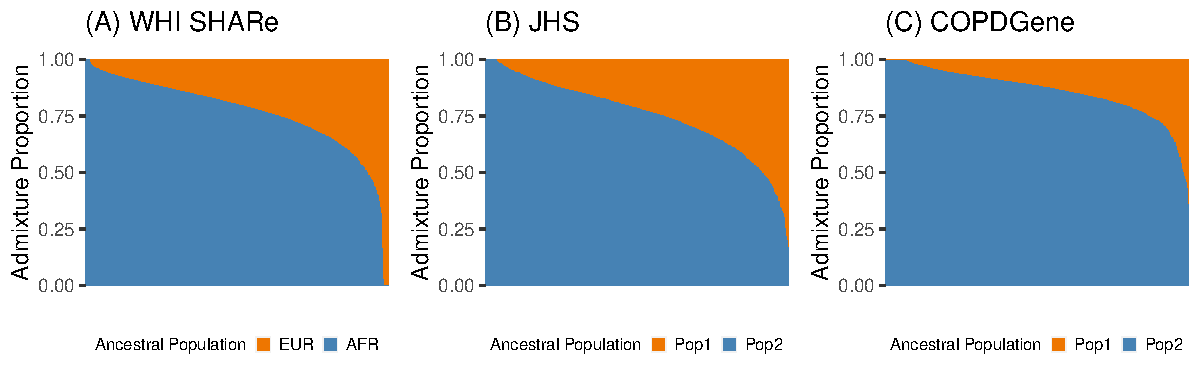
\includegraphics[width=\textwidth]{figs/barplots/figure1}
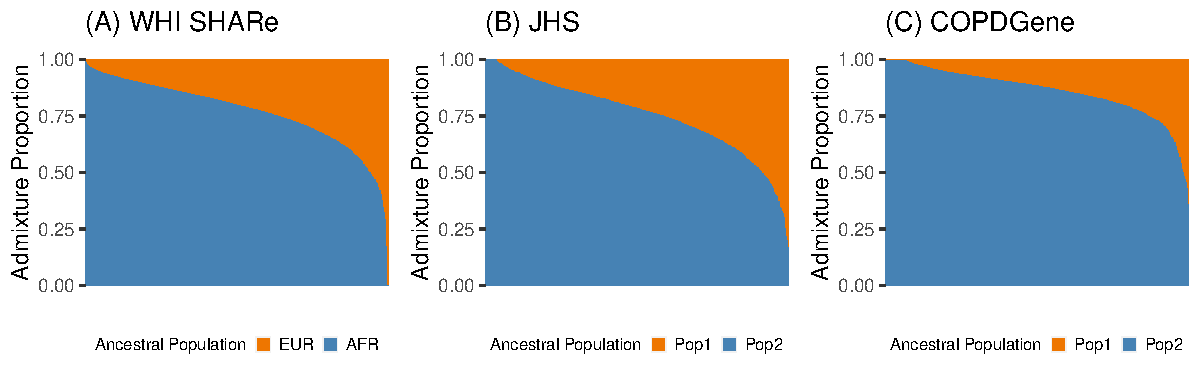
\includegraphics[width=\textwidth]{figs/barplots/barplots}
\caption{Barplots of estimated admixture proportions in (A) WHI SHARe, (B) TOPMed JHS, and (C) TOPMed COPDGene African Americans.}
\label{fig:barplots}
\end{figure}

In WHI SHARe African Americans, we compared admixture proportion estimates from a variety of model-based techniques. 
Figure \ref{fig:barplots} presents admixture proportions estimated as genome-wide average local ancestry, using local ancestry calls from \texttt{RFMix}. 
These local ancestry based admixture proportion estimates were highly correlated (Pearson correlation $>$ 0.998) with admixture proportions from supervised and unsupervised \texttt{ADMIXTURE} analyses with two ancestral populations ($K = 2$). 


%\begin{tabular}{l|rrrr}
%& avgLA  & unsupADM    & supADM & supPrunedADM \\
%\hline
%avgLA  &    1.0000000  &   0.9984003  &   0.9983740  &    0.9970080 \\
%unsupADM    &   0.9984003  &    1.0000000  &    0.9999973   &      0.9985752 \\
%supADM   &    0.9983740   &   0.9999973  &    1.0000000  &       0.9985835 \\
%supPrunedADM  &   0.9970080  &    0.9985752  &    0.9985835      &   1.0000000\\
%\end{tabular}

In TOPMed samples, we performed unsupervised \texttt{ADMIXTURE} analyses with varying numbers of ancestral populations. 
Figure \ref{fig:barplots} presents results with $K = 2$.
Although these analyses were unsupervised, based on prior studies of admixture in African Americans, and in comparison to the distribution of admixture proportions seen here in WHI SHARe, we believe that the ancestral population colored orange (Pop1) in Figure \ref{fig:barplots} corresponds to European ancestry and the population colored in blue (Pop2) corresponds to African ancestry.

In all three samples, we observe considerable variability in the relative proportions of African and European ancestry across individuals.
This ancestral heterogeneity motivates the need to carefully adjust for global ancestry in genome-wide association studies in these, just as in other, admixed samples. 

%\edit{
%\begin{itemize}
%\item Add WHI SHARe Hispanic Americans? (check with Tim)
%\item Possible supplemental figure: JHS and COPDGene with K = 3 (and/or K = 4 for COPDGene)
%\item Possible supplemental figure: JHS and COPDGene barplots before filtering out European Americans
%\end{itemize}
%}


\subsection{First PC captures global ancestry}

\begin{figure}
\center
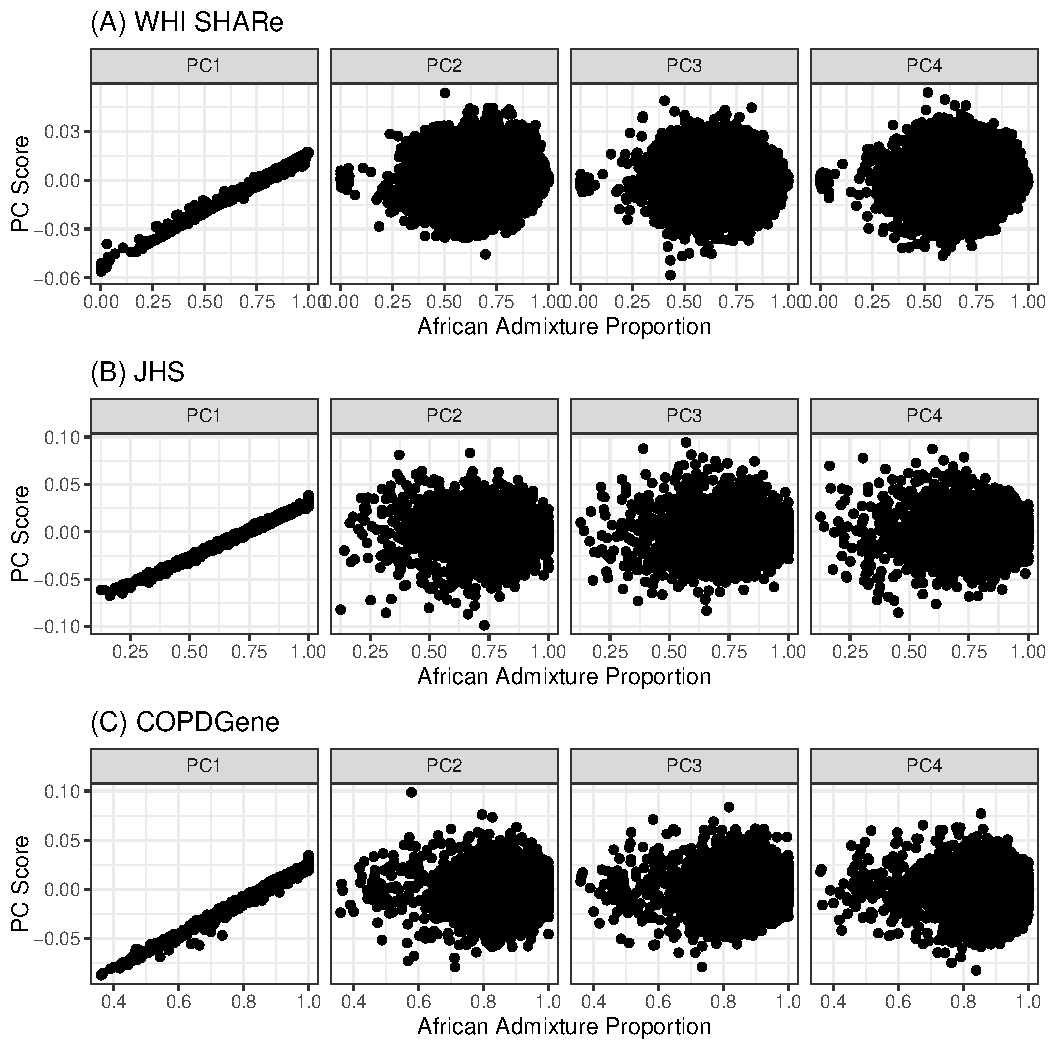
\includegraphics[width=\textwidth]{figs/pcs_vs_global/pcs_vs_global}
\caption{Scatterplots of estimated African admixture proportions versus the first four PCs in (A) WHI SHARe, (B) TOPMed JHS, and (C) TOPMed COPDGene African Americans. Here we consider PCs that were generated without any prior LD-based filtering or pruning.}
\label{fig:pcsvsglob}
\end{figure}

In an African American population, we might expect that only one principal component is needed to capture ancestral heterogeneity, at least with respect to differences in the relative proportion of African and European continental ancestry. 
Comparing model-based admixture proportions to principal components in WHI SHARe, JHS, and COPDGene confirms this hypothesis. 
In all three samples of African Americans, the first principal component is highly correlated with the inferred proportion of African ancestry, while later PCs show very little correlation with genome-wide continental ancestry (Figure \ref{fig:pcsvsglob}).
We observe similar patterns of correlation between PCs and inferred admixture proportions regardless of the type of LD filtering (or lack therof) performed prior to running PCA (Supplemental Figure \ref{fig:prunedpcsvsglob}). 


\subsection{Later PCs may capture local genomic features}
\label{sec:CorrPlots}

%\noindent See Figure \ref{fig:corr-TOPMed} for PC-genotype correlation with naive PCs in JHS and COPDGene African Americans, and Supplemental Figure \ref{fig:corr-Eur} shows the same (except loadings instead of correlation) in COPDGene European Americans.
%
%\noindent See Figure \ref{fig:corr-compare} for a comparison of naive PCs vs exclusions vs stricter-than-default pruning vs both in WHI SHARe.
%
%\noindent See Supplemental Figures \ref{fig:corr-compare-prune}, \ref{fig:corr-compare-window}, and \ref{fig:corr-compare-exclude} for comparisons of PCs with different choices of $r^2$ thresholds (for pruning), different choices of window sizes (for pruning), and multiple iterations of data-based exclusions, respectively.


%% what do we see with no pruning
As we see in Figure \ref{fig:pcsvsglob}, in African American samples the first principal component seems to be capturing global ancestry, whereas later PCs are not.
While it is possible that these higher-order principal components may be capturing sub-continental structure that is not captured by the model-based admixture proportions, we see in many cases that these later PCs are actually capturing local genomic features rather than genome-wide ancestry. 
This is evident upon inspection of \textit{SNP loadings}, which represent the contribution of each variant to each principal component, or in investigating the correlation between principal component scores and the original genotypes.

Figure \ref{fig:corr-TOPMed} presents the correlation between principal components and genotypes in JHS and COPDGene African Americans when PCs are generated without any prior LD-based pruning or filtering.
We see that variants across the genome are contributing relatively equally to the first principal component, whereas the second, third, and fourth PCs are driven more-so by variants on a select number of chromosomes.
In JHS, for example, the second PC is particularly highly correlated with variants on chromosomes 6 and 8, and less so with variants on 2, 3, and 11.
We see similar patterns, although with peaks on different combinations of chromosomes, in COPDGene (Figure \ref{fig:corr-TOPMed}B) and WHI SHARe African Americans (leftmost column of Figure \ref{fig:corr-compare}).
The peaks in these genotype-PC correlation plots indicate that those principal components are primarily capturing variation at a handful of positions along the genome rather than genome-wide global ancestry.

Note that these patterns differ slightly from what has previously been observed in European populations.
In particular, in European populations a principal component might capture variation on a single chromosome (e.g., see Supplemental Figure \ref{fig:corr-Eur}), whereas here in these admixed populations we see PCs driven by contributions from variants across several chromosomes.

\begin{figure}
\hspace{0.3in} (A) JHS \hspace{2.4in} (B) COPDGene
\center
\includegraphics[width=0.49\textwidth]{figs/JHS/JHS_prune_FALSE_1_0_0.01_snprelate_corr_1}
\includegraphics[width=0.49\textwidth]{figs/COPD/COPD_prune_FALSE_1_0_0.01_snprelate_corr_1}
\caption{Correlation between naively generated PCs (i.e., PCs that were constructed without any prior LD-based filtering or exclusions) and genotypes in JHS and COPDGene African Americans. Each panel plots the absolute value of the correlation between principal components and genotypes (on the y-axis) versus the position along the genome (x-axis).  Panels are organized vertically according to which PC is being investigated (1, 2, 3, 4) and horizontally according to the sample (A: JHS, B: COPDGene). Peaks in this plot indicate that a variant has a larger \textit{loading}, i.e., a larger contribution to that principal component.}
\label{fig:corr-TOPMed}
\end{figure}


\subsection{Impact of LD pruning}

%% why is this happening [very brief] + what happens with LD pruning
Previous authors have suggested that this phenomenon of principal components capturing local genomic features arises due to high or otherwise unusual patterns of linkage disequilibrium among variants; as a result, they recommend that variants in high LD with one another be removed prior to running PCA. 
Following these recommendations, we compare the set of principal components based on all variants to PCs generated after first removing regions of the genome known to have high LD (Table \ref{tab:highLD}), performing LD pruning, or both. 

Figure \ref{fig:corr-compare} illustrates the impact of these pre-processing steps on the correlation between genotypes and PCs in WHI SHARe African Americans. 
Recall that the leftmost column of Figure \ref{fig:corr-compare} presents results for principal components that were generated without any prior LD-based filtering or pruning, and we see that PCs 2--4 are capturing local genomic features on a select number of chromosomes rather than genome-wide ancestry.
When we exclude the previously-identified high LD regions reported in Table \ref{tab:highLD} before running PCA (the second column of Figure \ref{fig:corr-compare}), the pattern of \textit{which} SNPs are driving PCs 2--4 changes, but the issue of PCs capturing local genomic features has not been resolved. 
However, after LD pruning with an $r^2$ threshold of 0.1 and a window size of 0.5 Mb (third column), we now see similar patterns with PCs 2--4 as we do with the first principal component --- all variants are now contributing relatively equally to each PC. 
If we then also remove previously-identified high LD regions in addition to performing LD pruning (rightmost column), the patterns of correlation between PCs and genotypes are indistinguishable from those with LD pruning alone. 

Note that the thresholds for LD pruning that we use here ($r^2 < 0.1$) are stricter than the default for many software programs and the threshold used in many studies of European populations ($r^2 < 0.2$).
If we use this default $r^2$ threshold, we see improvement for the second and third principal components, but the fourth continues to capture local genomic features on a small number of chromosomes (Supplemental Figure \ref{fig:corr-compare-prune}). 
Similar patterns are observed in JHS and COPDGene.

\begin{figure}
\center
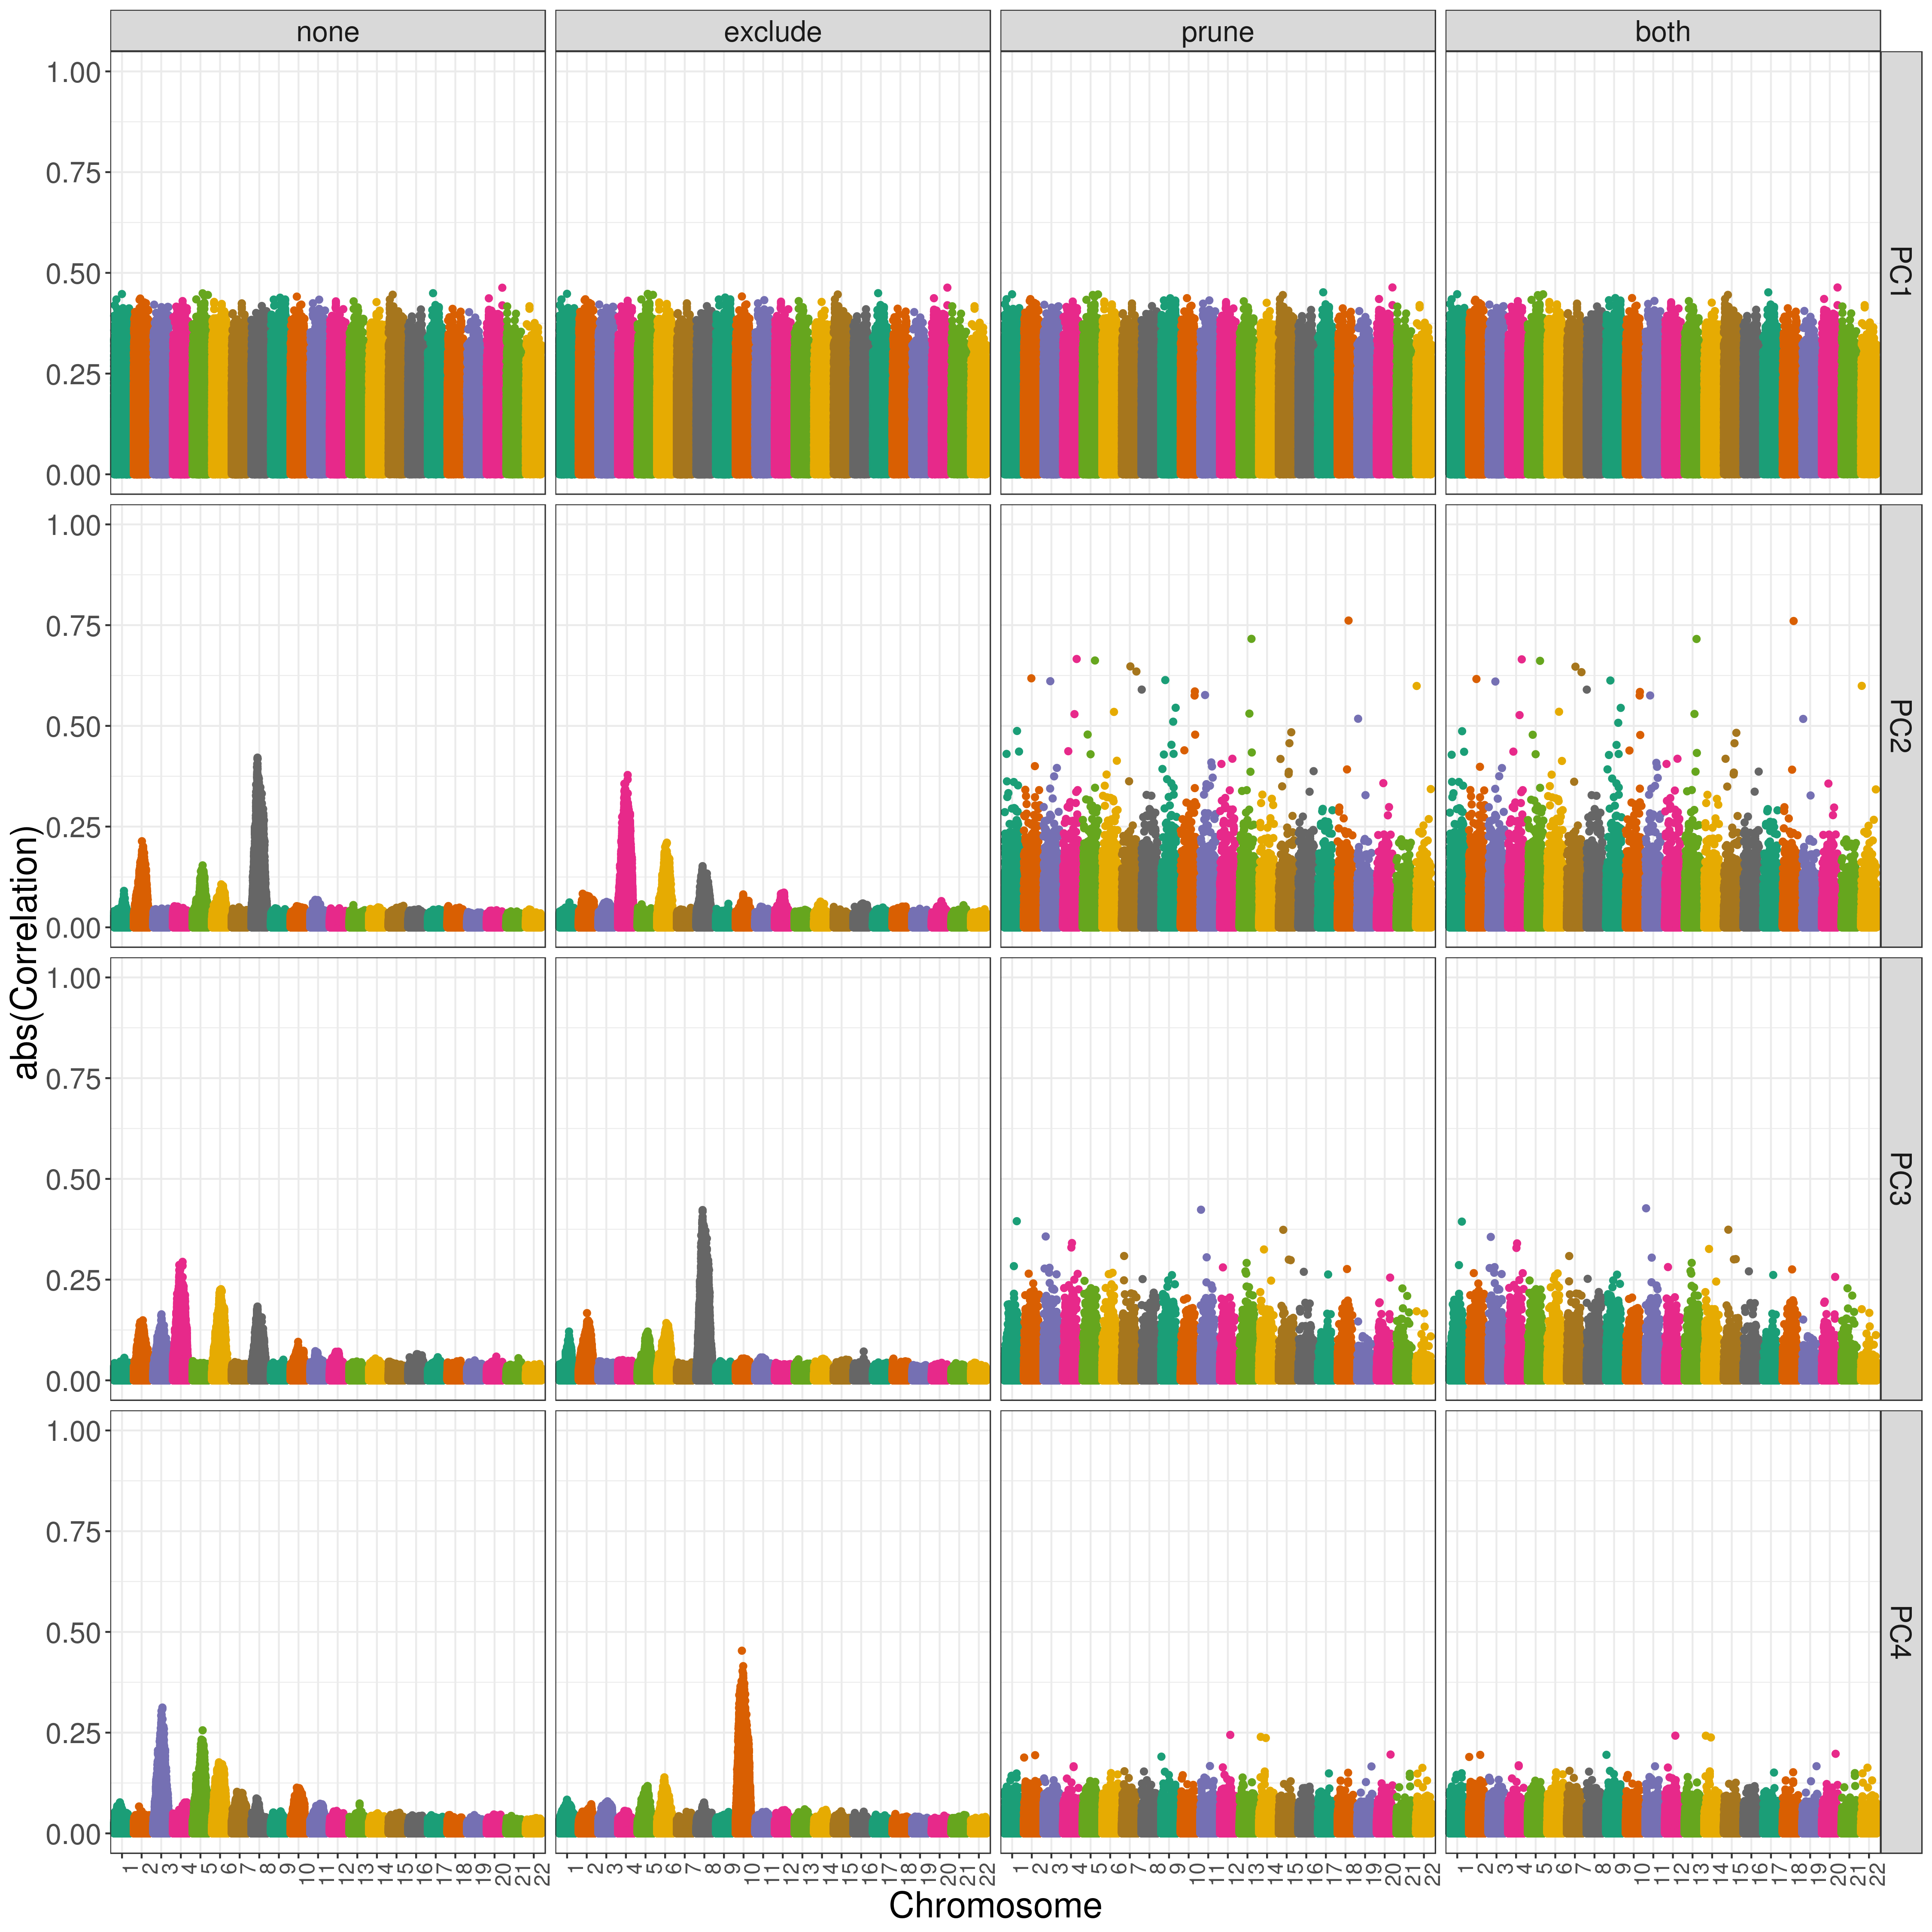
\includegraphics[width=\textwidth]{figs/pc_geno_corr/pc_geno_corr}
\caption{Correlation between PCs and genotypes in WHI SHARe African Americans with different choices of pre-processing. Each panel plots the absolute value of the correlation between principal components and genotypes (on the y-axis) versus the position along the genome (x-axis).  Panels are organized vertically according to which PC is being investigated (1, 2, 3, 4) and horizontally according to the level of filtering that was applied prior to running PCA (\textit{none}: all SNPs, \textit{exclude}: after excluding regions in Table \ref{tab:highLD}, \textit{prune}: after LD pruning with an $r^2$ threshold of 0.1 and window size of 0.5 Mb, and \textit{both}: after both exclusions and LD pruning).}
\label{fig:corr-compare}
\end{figure}


%\begin{figure}[h]
%\caption{Correlation between PCs and genotypes in WHI SHARe African Americans. \\Each panel plots the absolute value of the correlation (y-axis) between principal components and genotypes at each position along the genome (x-axis). Panels are stratified according to which PC is being investigated (1, 2, 3, or 4) and what level of LD filtering was applied prior to running PCA: \textit{none} (all SNPs), \textit{exclude} (after excluding regions in Table \ref{tab:highLD}), \textit{prune} (after LD pruning with an $r^2$ threshold of 0.1 and a window size of 0.5 Mb, or \textit{both} (after exclusions and LD pruning).}
%\label{fig:corrWHI}
%\end{figure}


%\begin{figure}
%\label{fig:corrNoExclude}
%\makebox[\textwidth][c]{
%\includegraphics[width=0.24\paperwidth]{figs/JHS_prune_FALSE_1_0_0.01_snprelate_corr_1}
%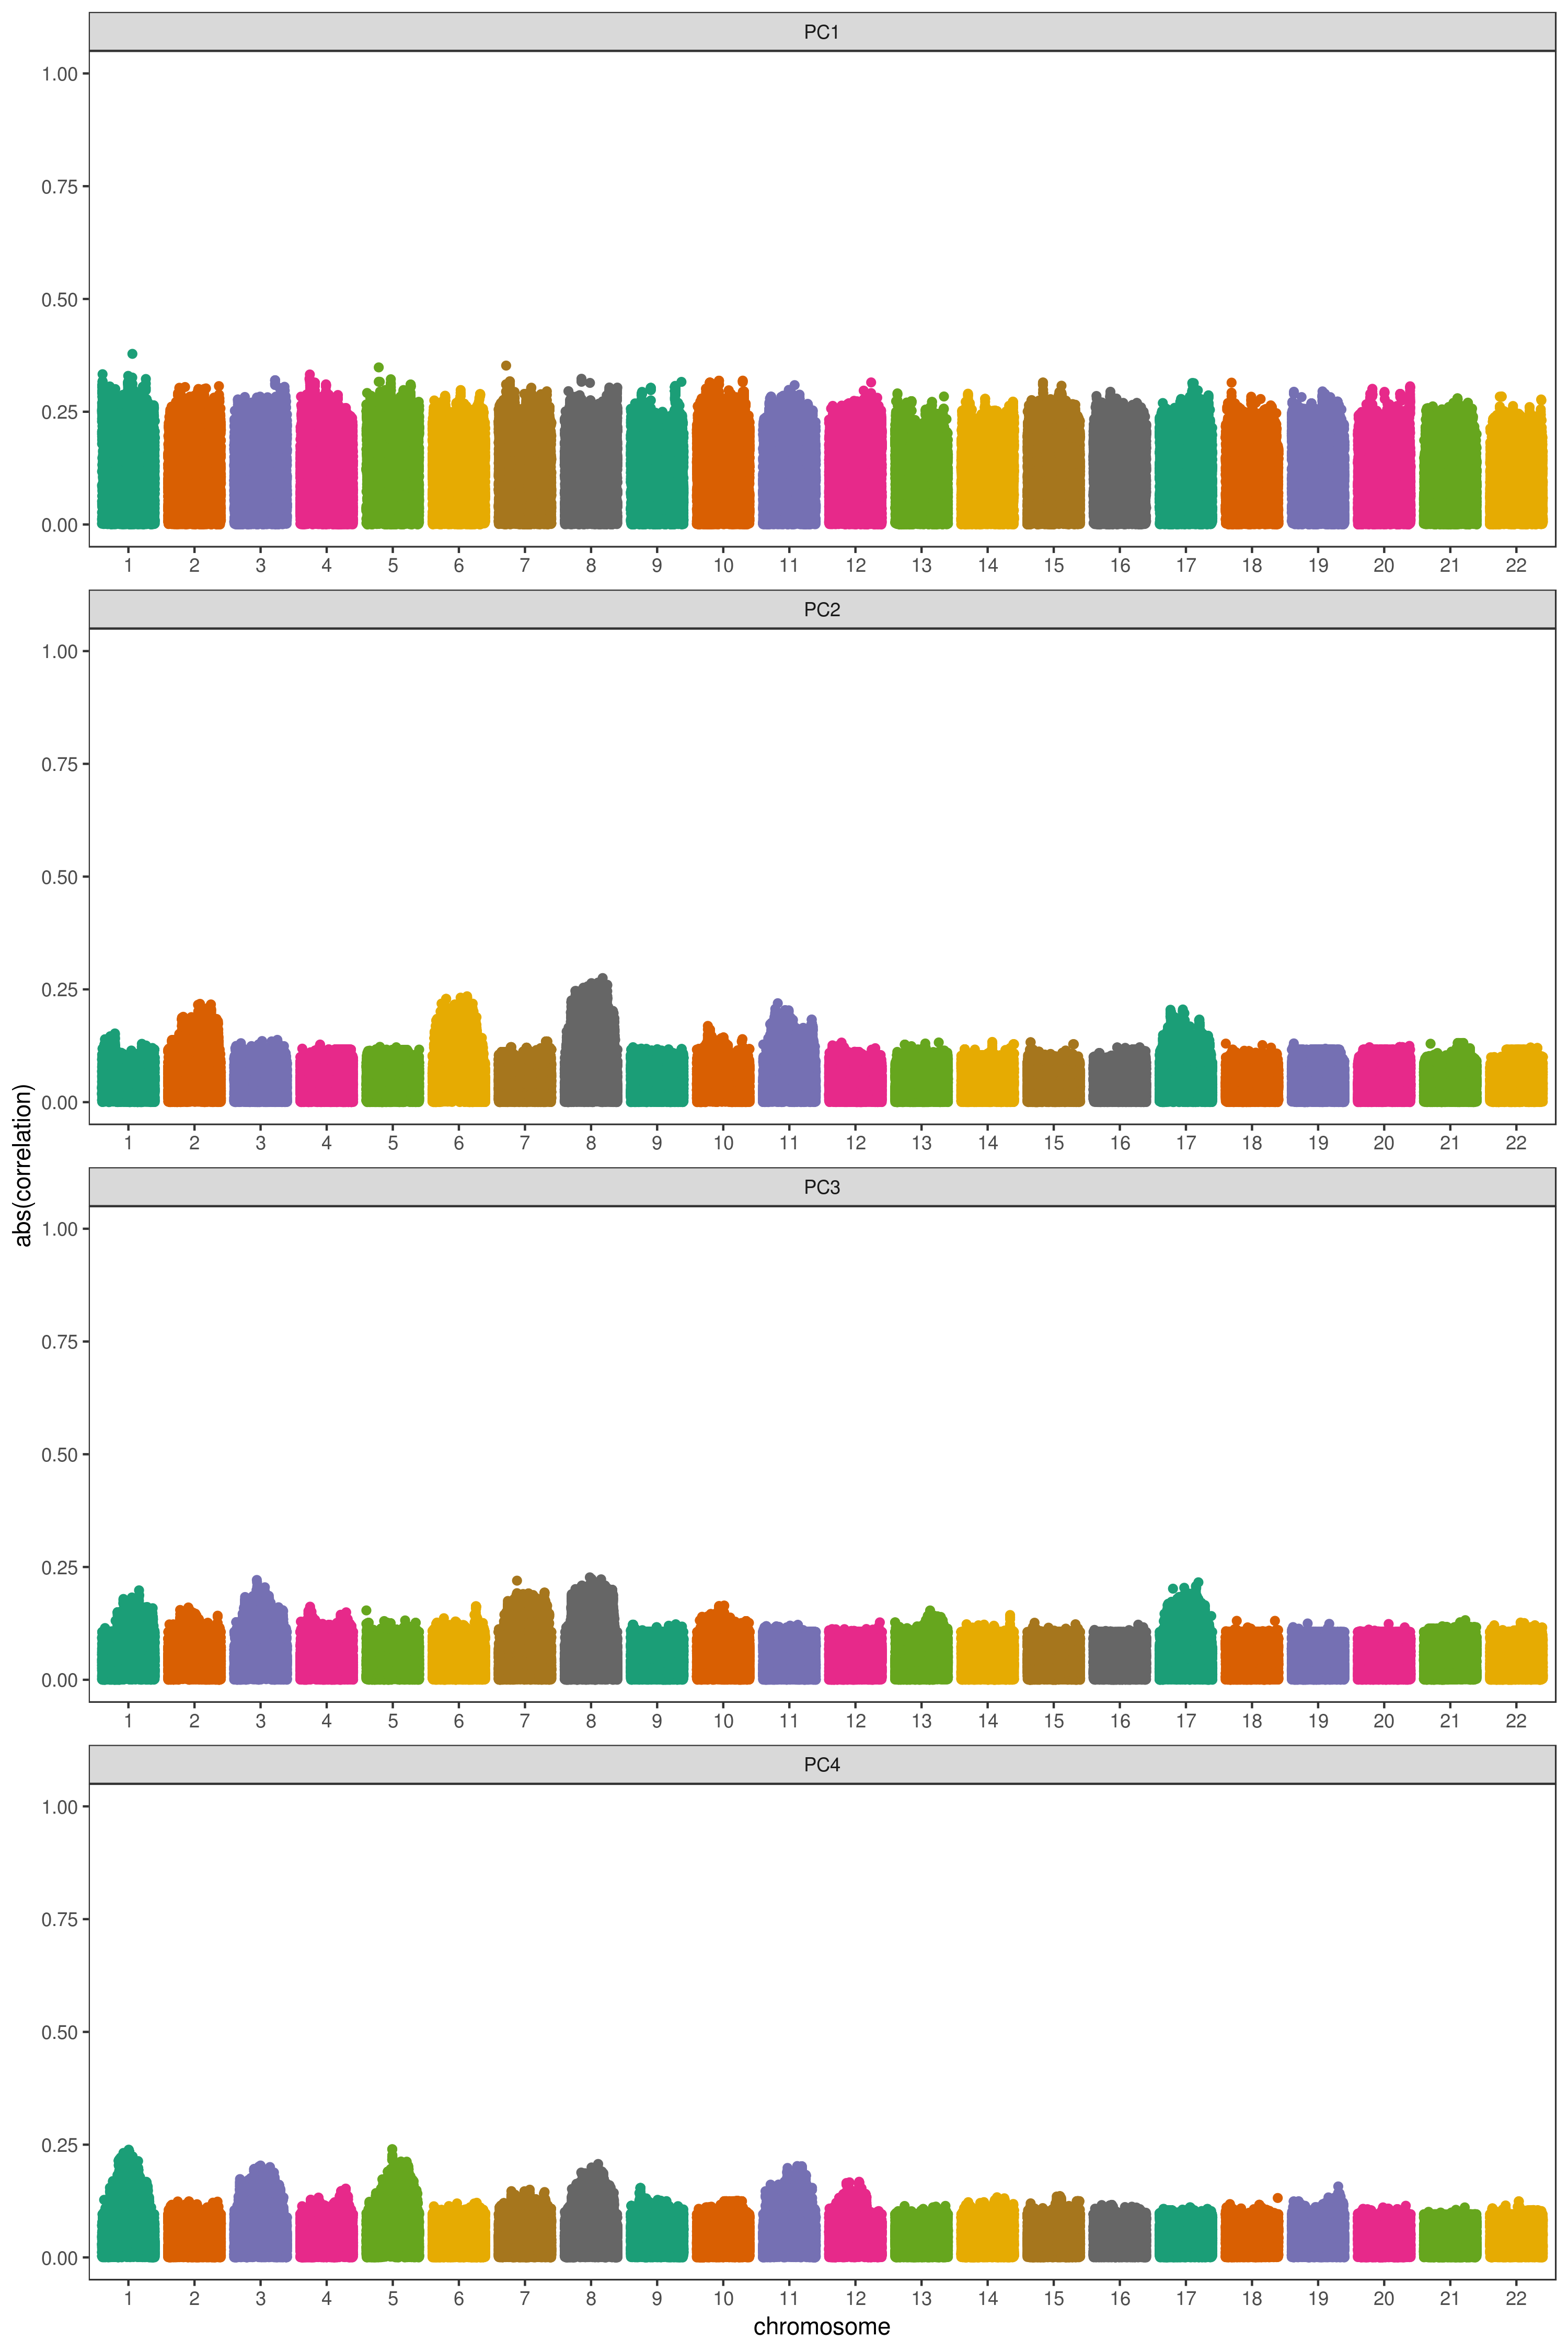
\includegraphics[width=0.24\paperwidth]{figs/JHS_prune_FALSE_0.2_0.5_0.01_snprelate_corr_1}
%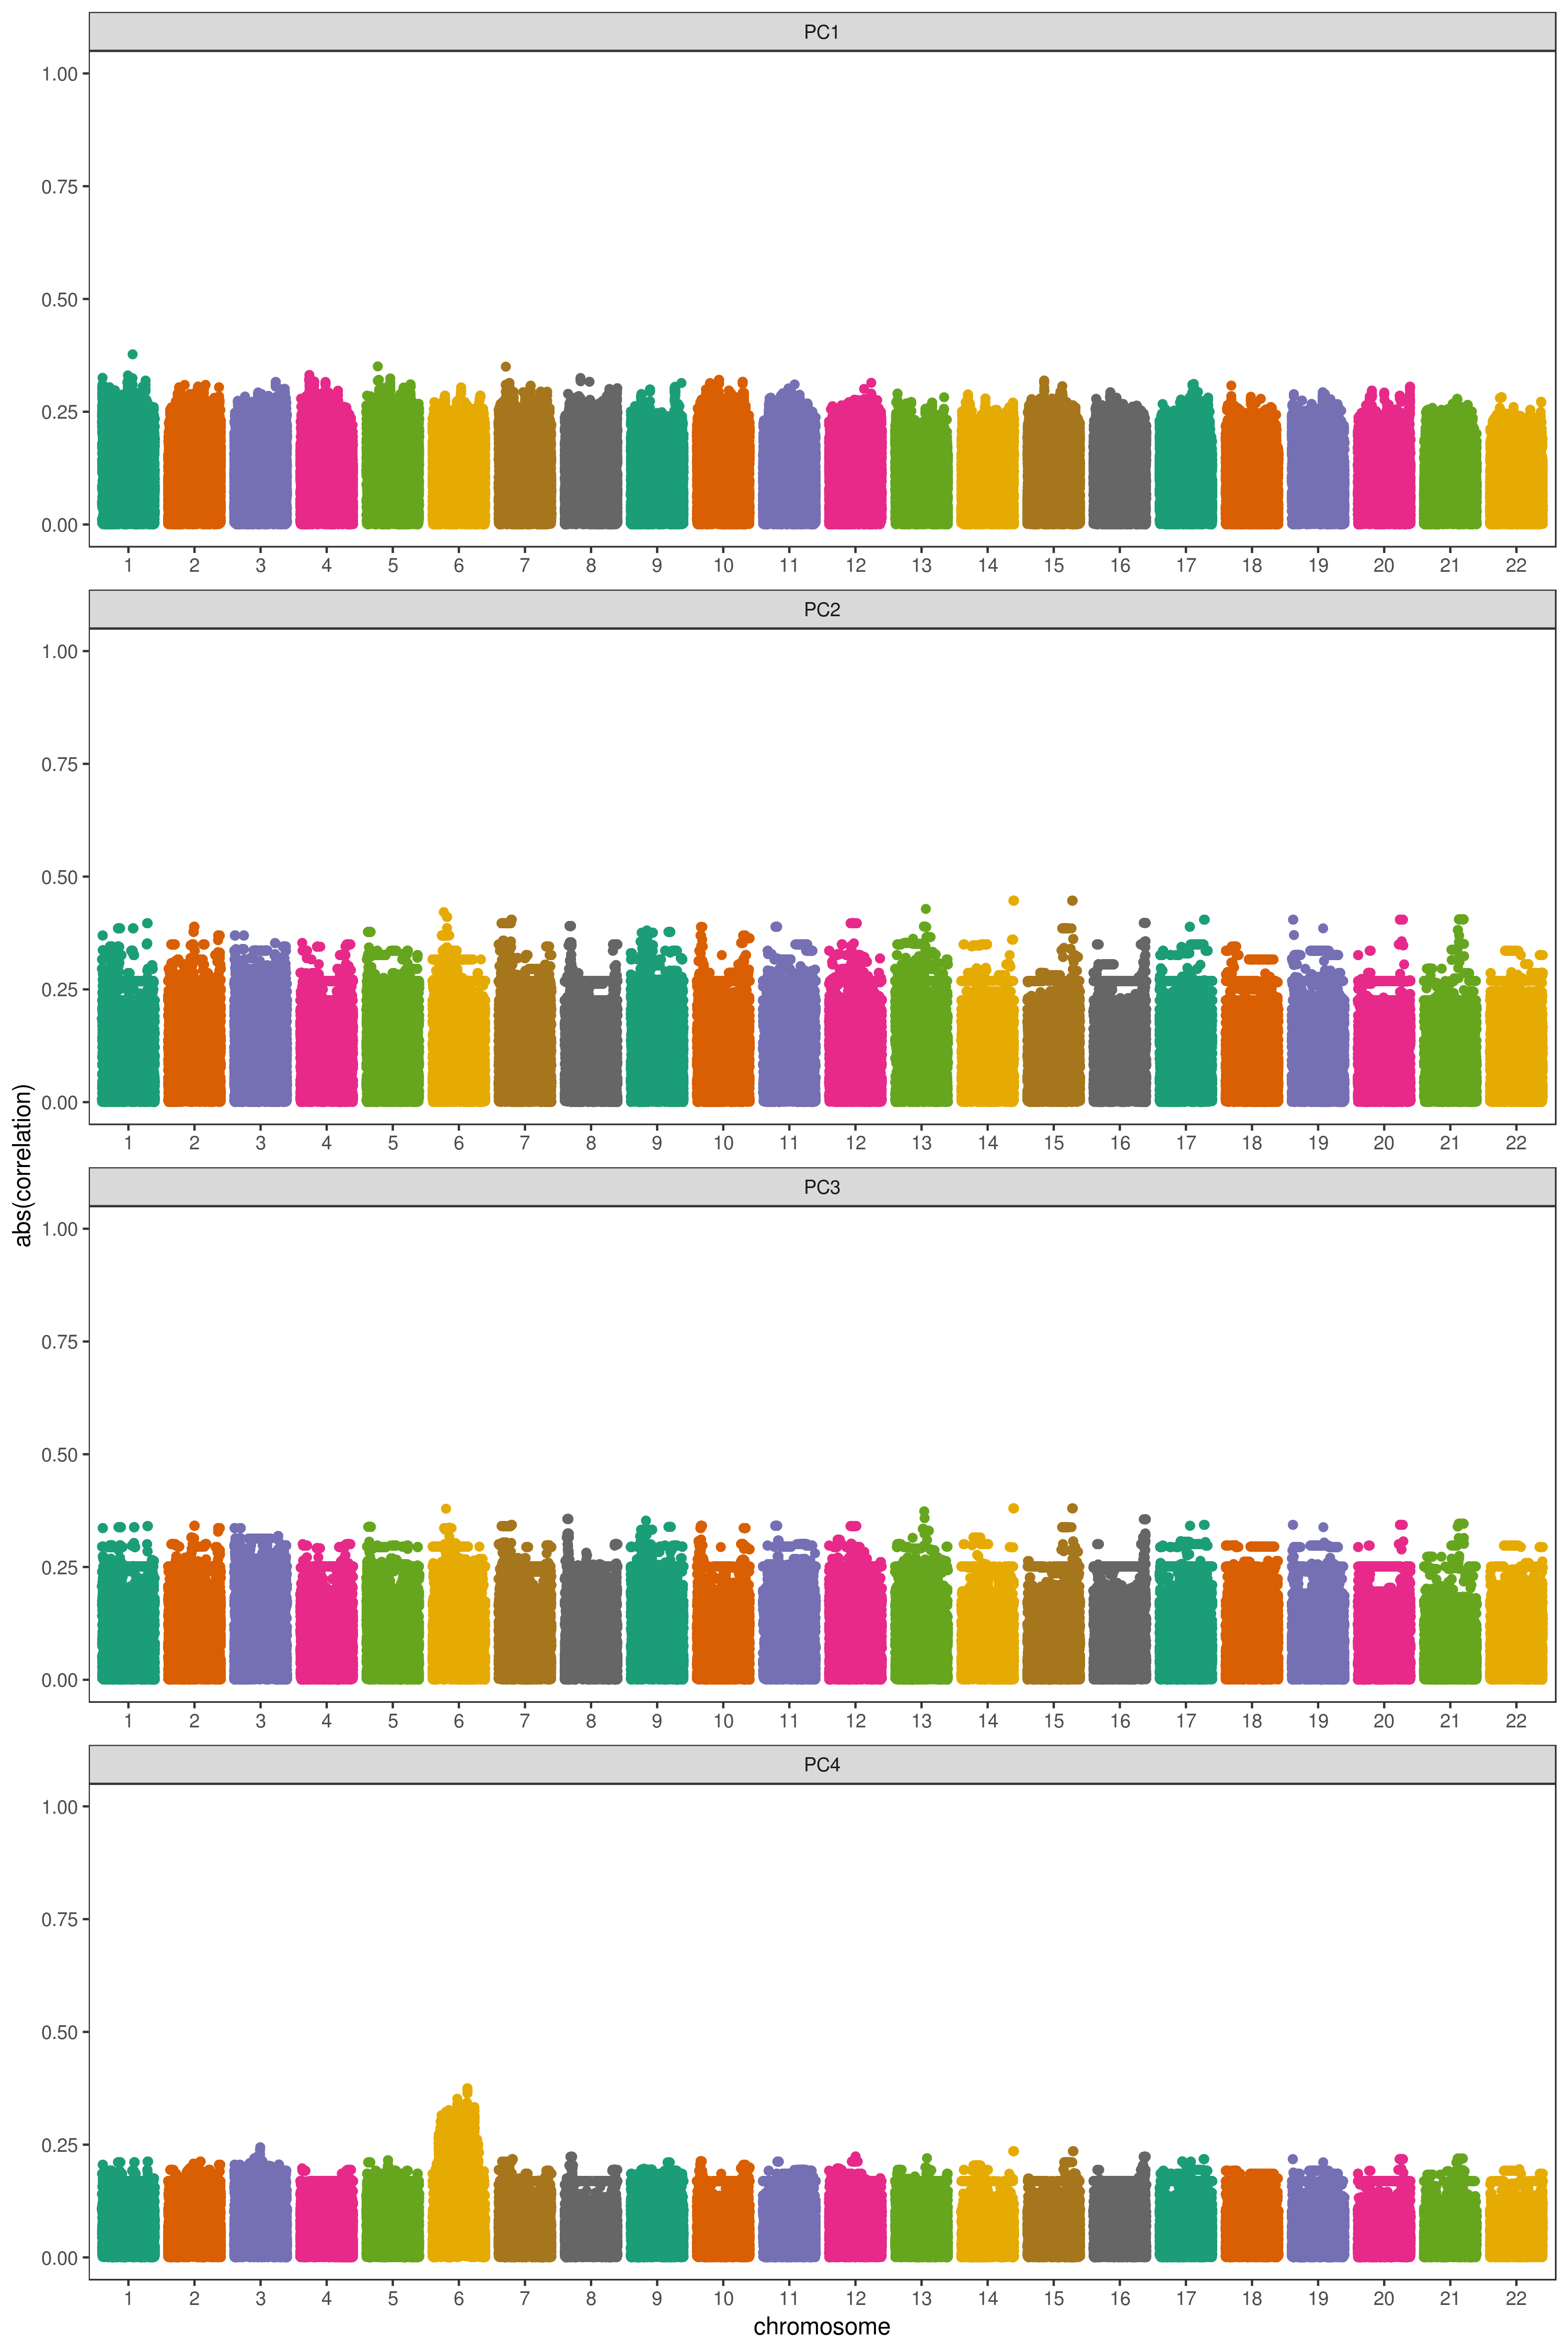
\includegraphics[width=0.24\paperwidth]{figs/JHS_prune_FALSE_0.1_0.5_0.01_snprelate_corr_1}
%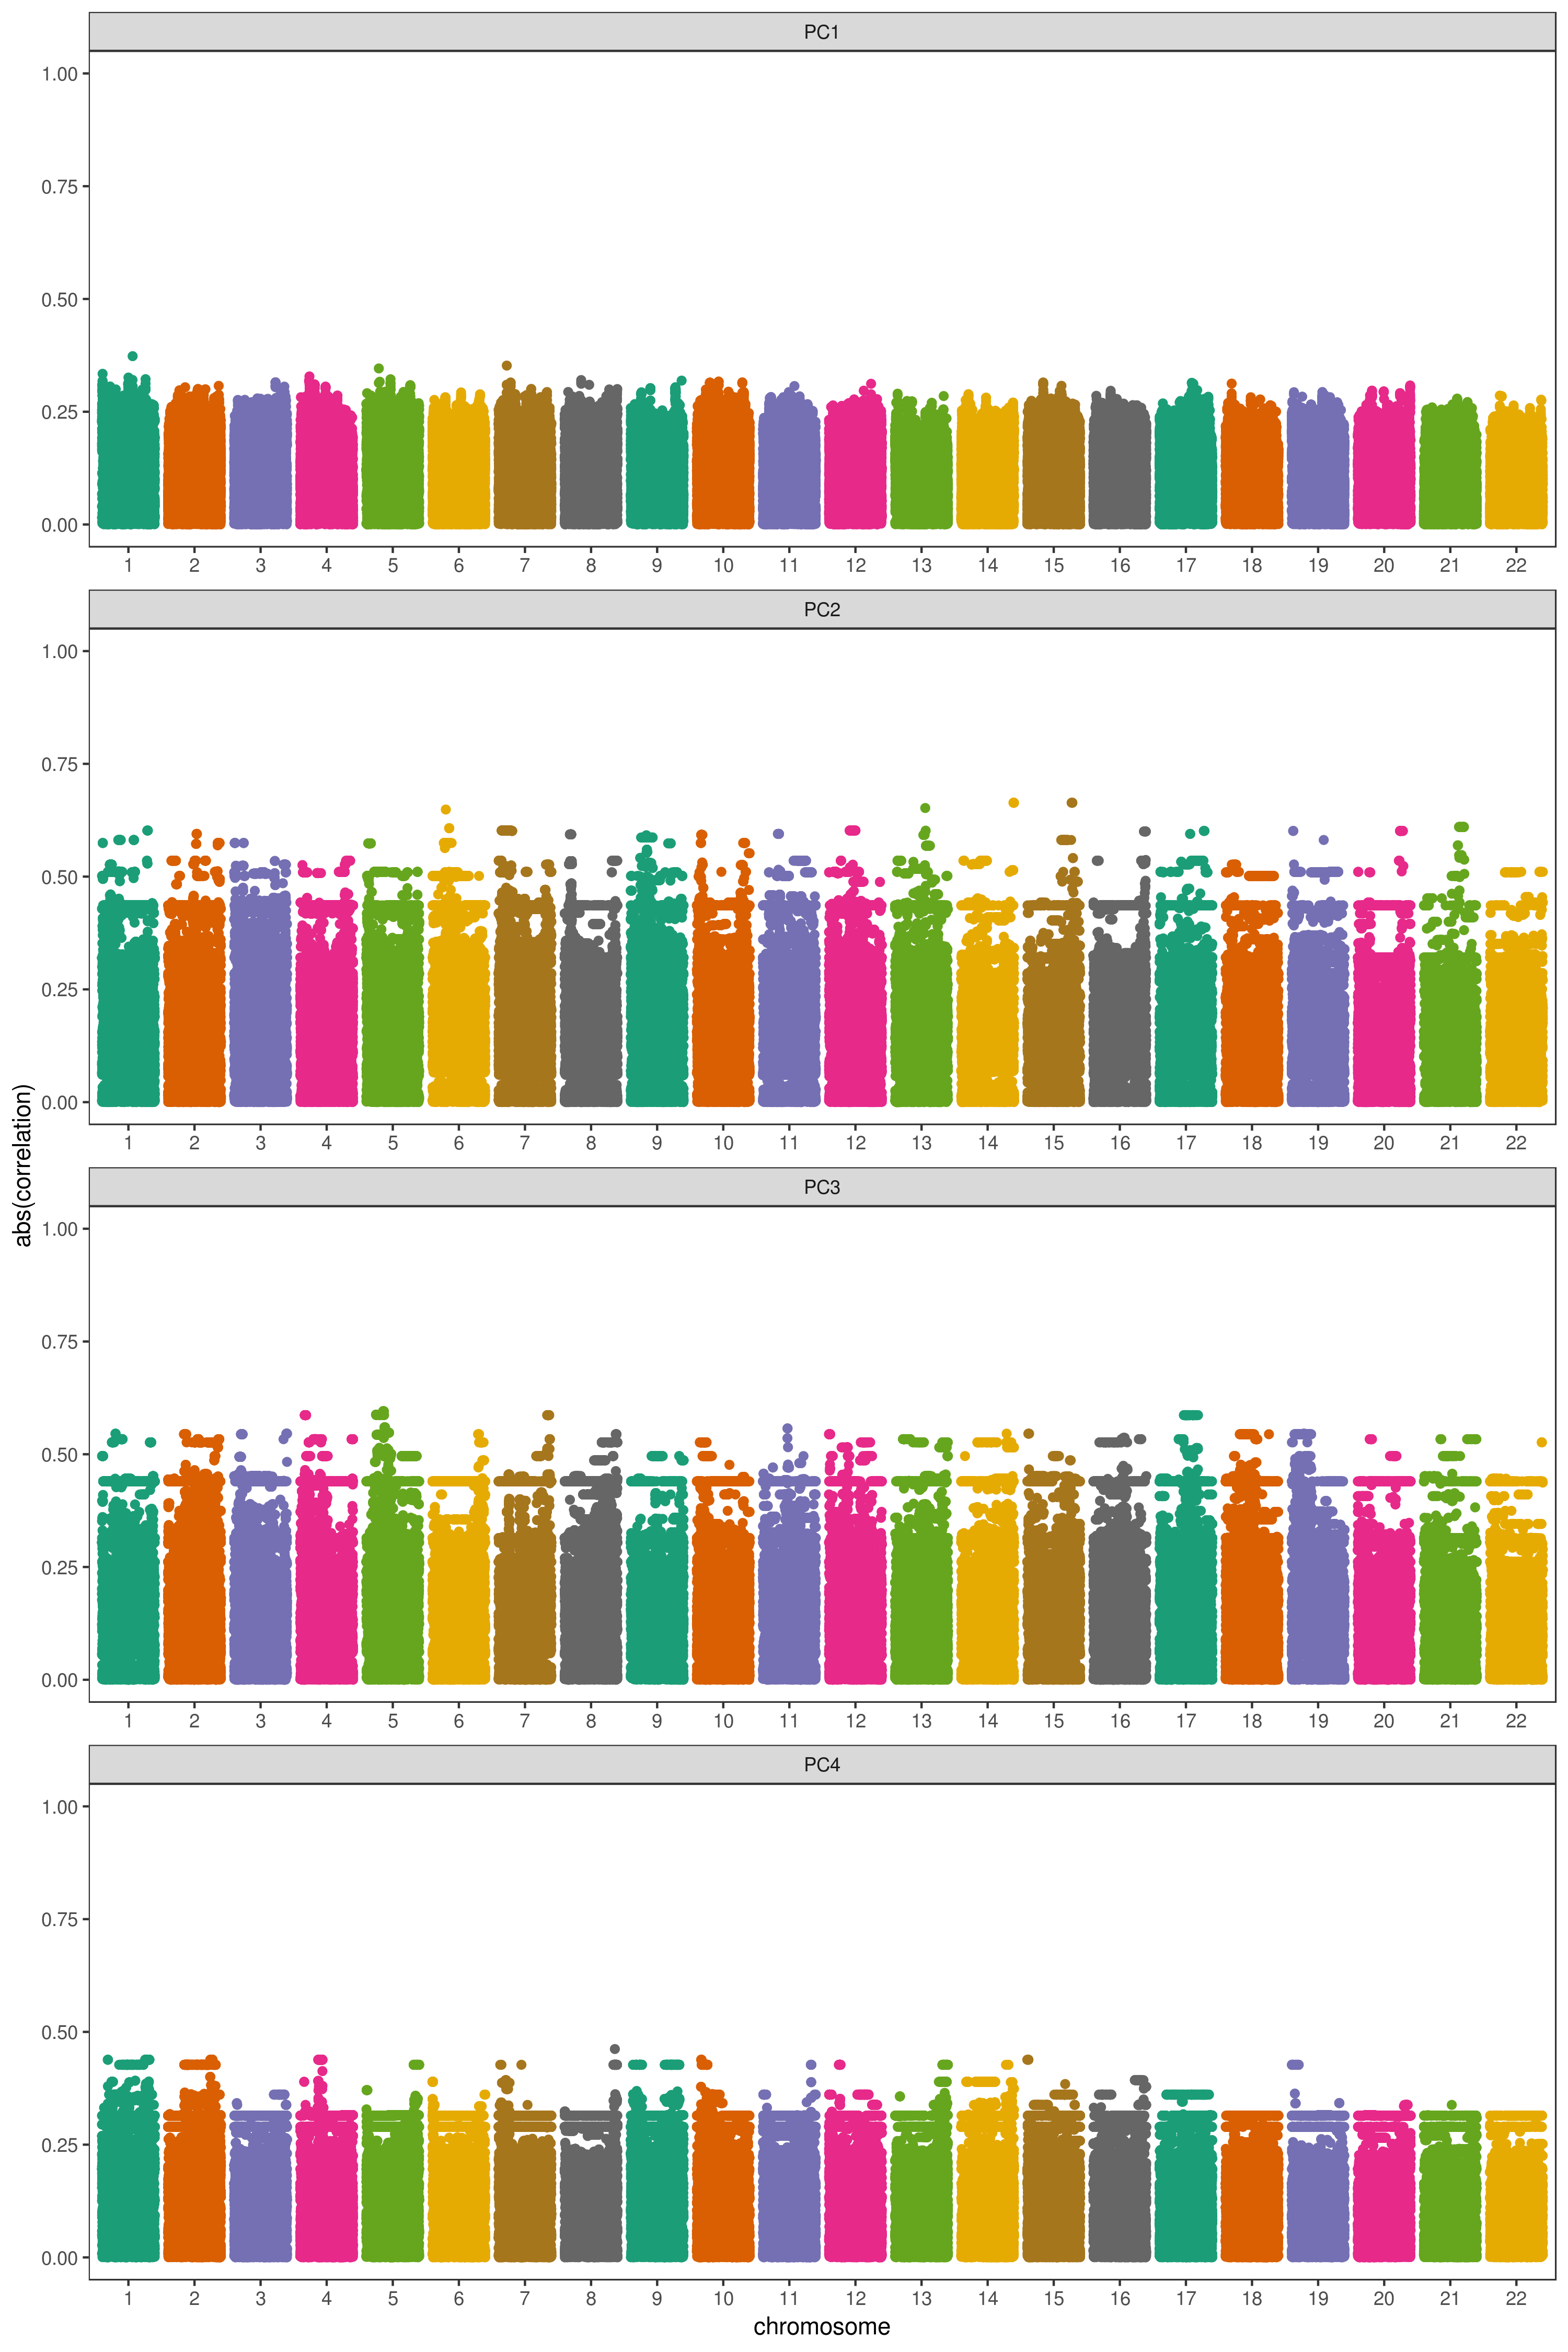
\includegraphics[width=0.24\paperwidth]{figs/JHS_prune_FALSE_0.1_10_0.01_snprelate_corr_1}
%}
%\caption{Correlation between the first four principal components and genotypes in Jackson Heart Study African Americans when previously-identified high-LD regions (Table \ref{tab:highLD}) \textit{are not} removed prior to analysis. From left to right, panels correspond to increasingly strict levels of LD pruning: no LD pruning, LD pruning with an $r^2$ threshold of 0.2 and a window size of 0.5 Mb, LD pruning with an $r^2$ threshold of 0.1 and a window size of 0.5 Mb, and LD pruning with an $r^2$ threshold of 0.1 and a window size of 10 Mb.}
%\end{figure}

%\begin{figure}
%\label{fig:corrExclude}
%\makebox[\textwidth][c]{
%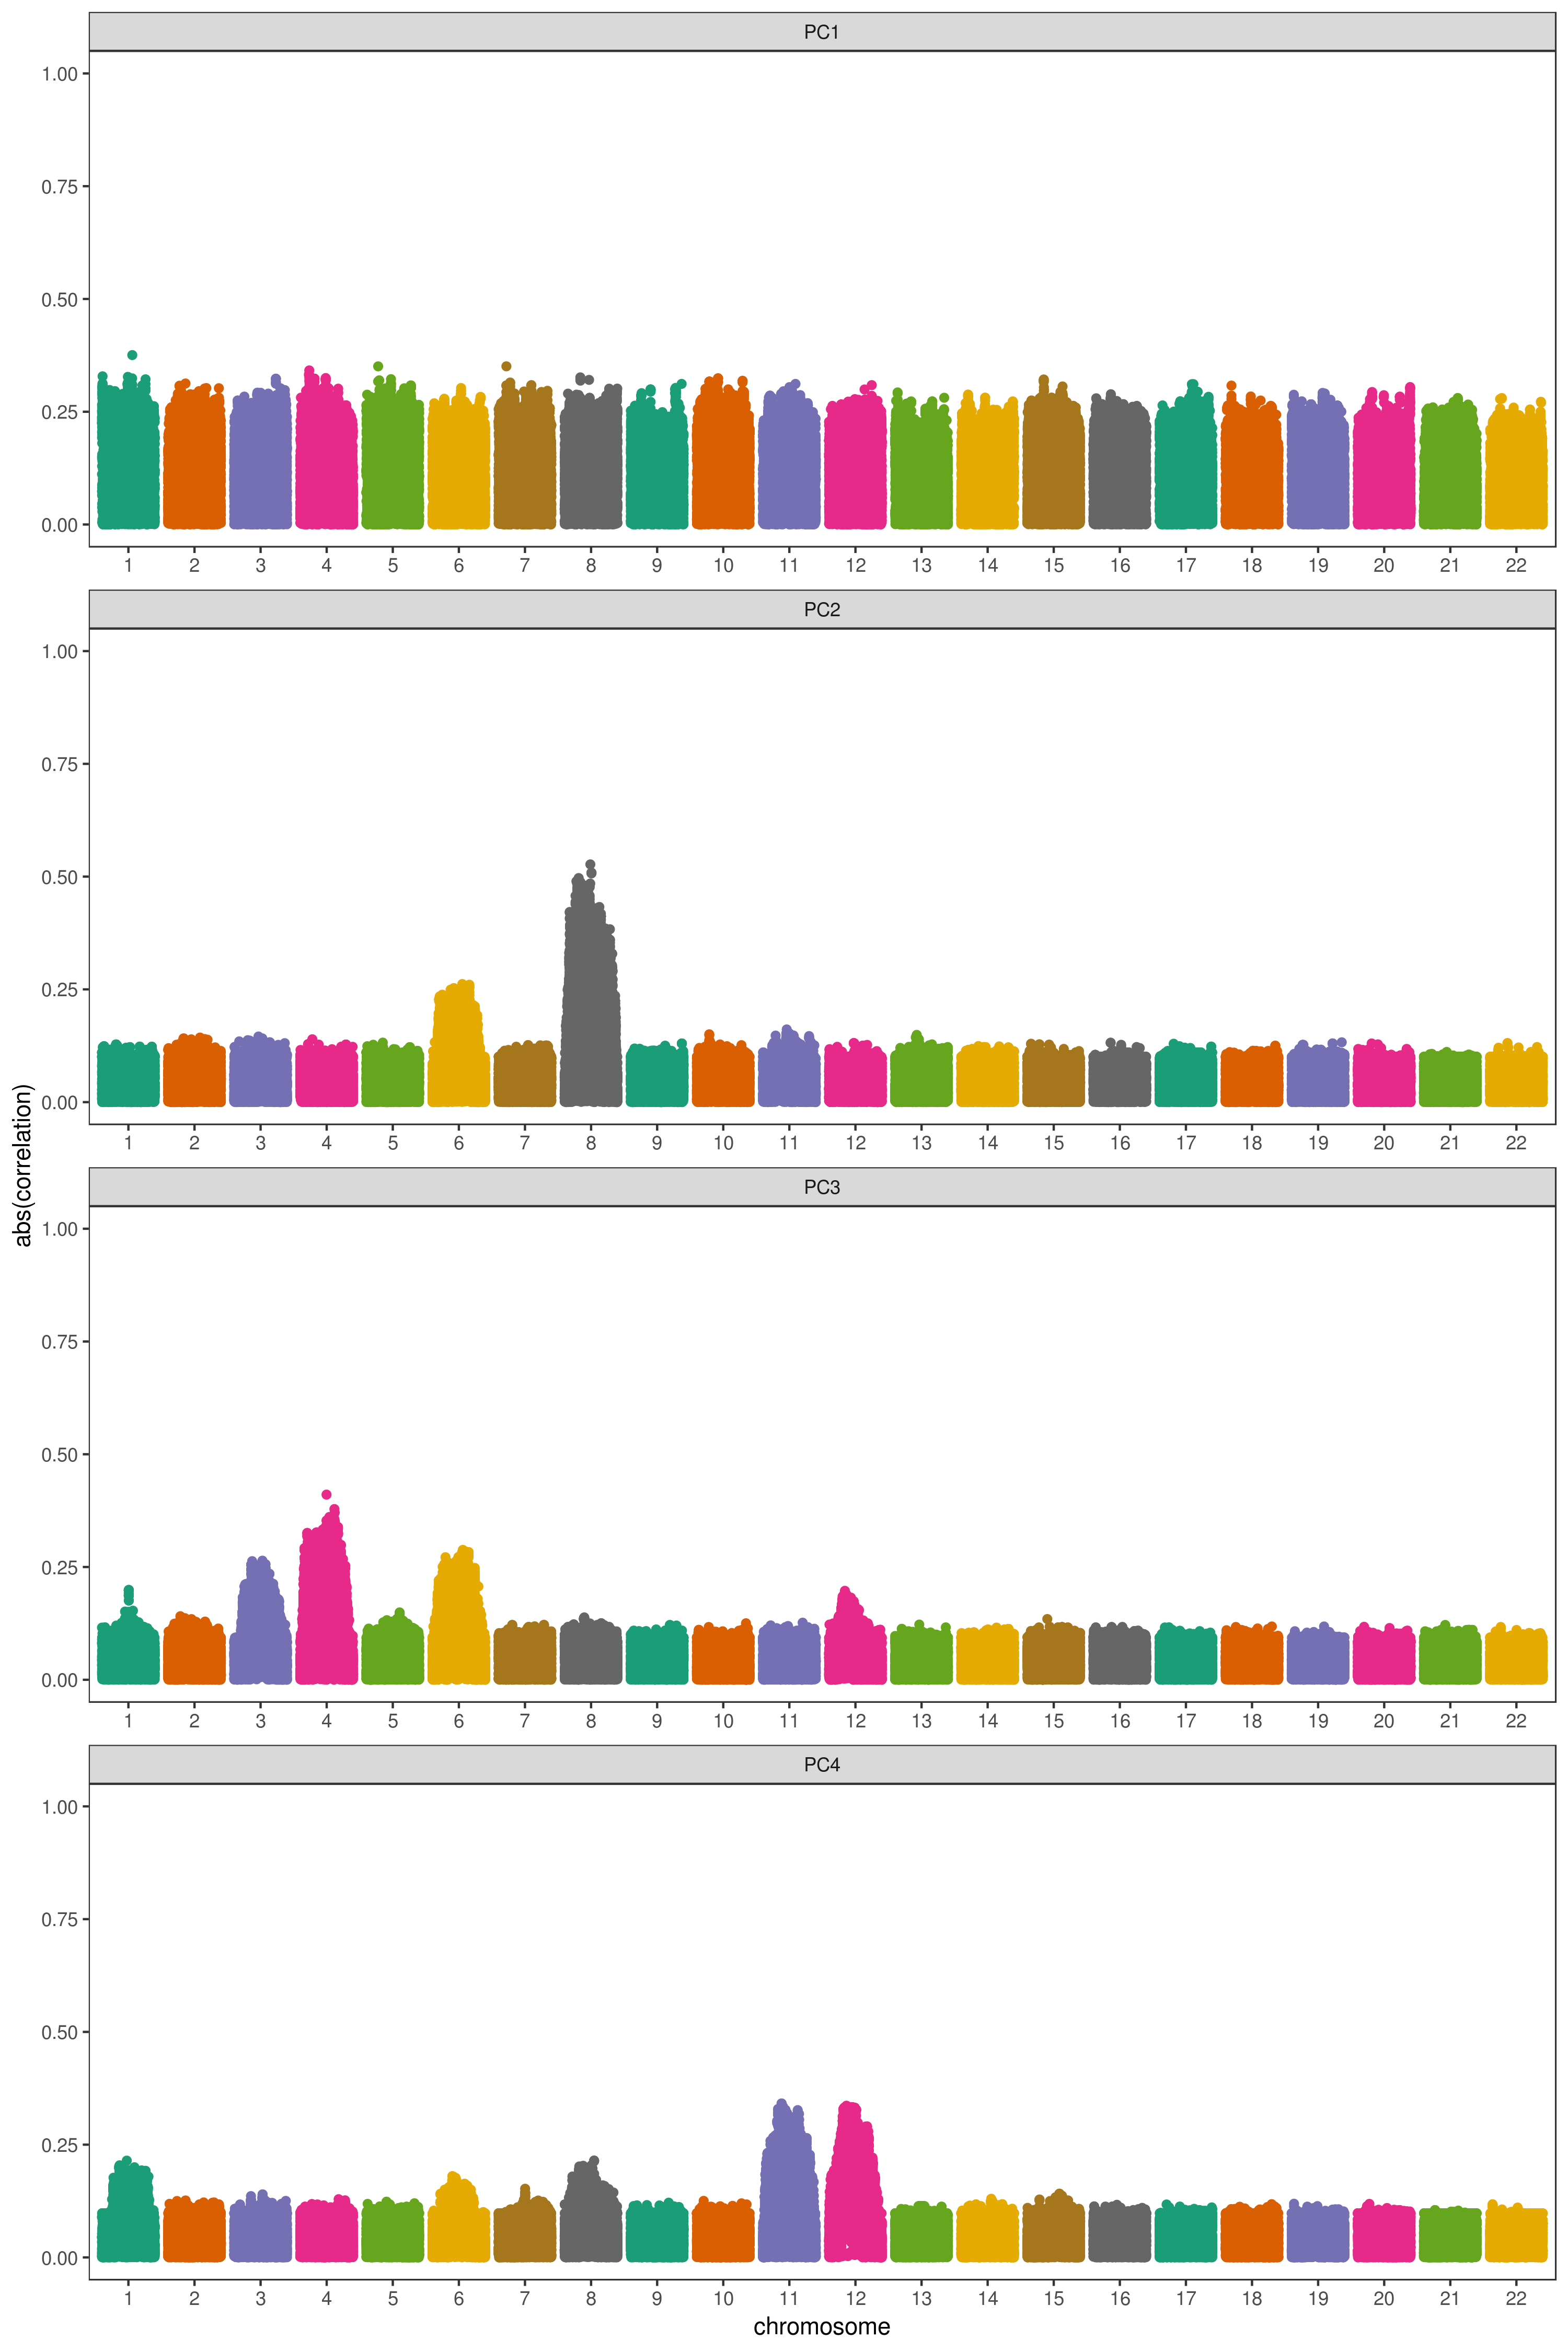
\includegraphics[width=0.24\paperwidth]{figs/JHS_prune_TRUE_1_0_0.01_snprelate_corr_1}
%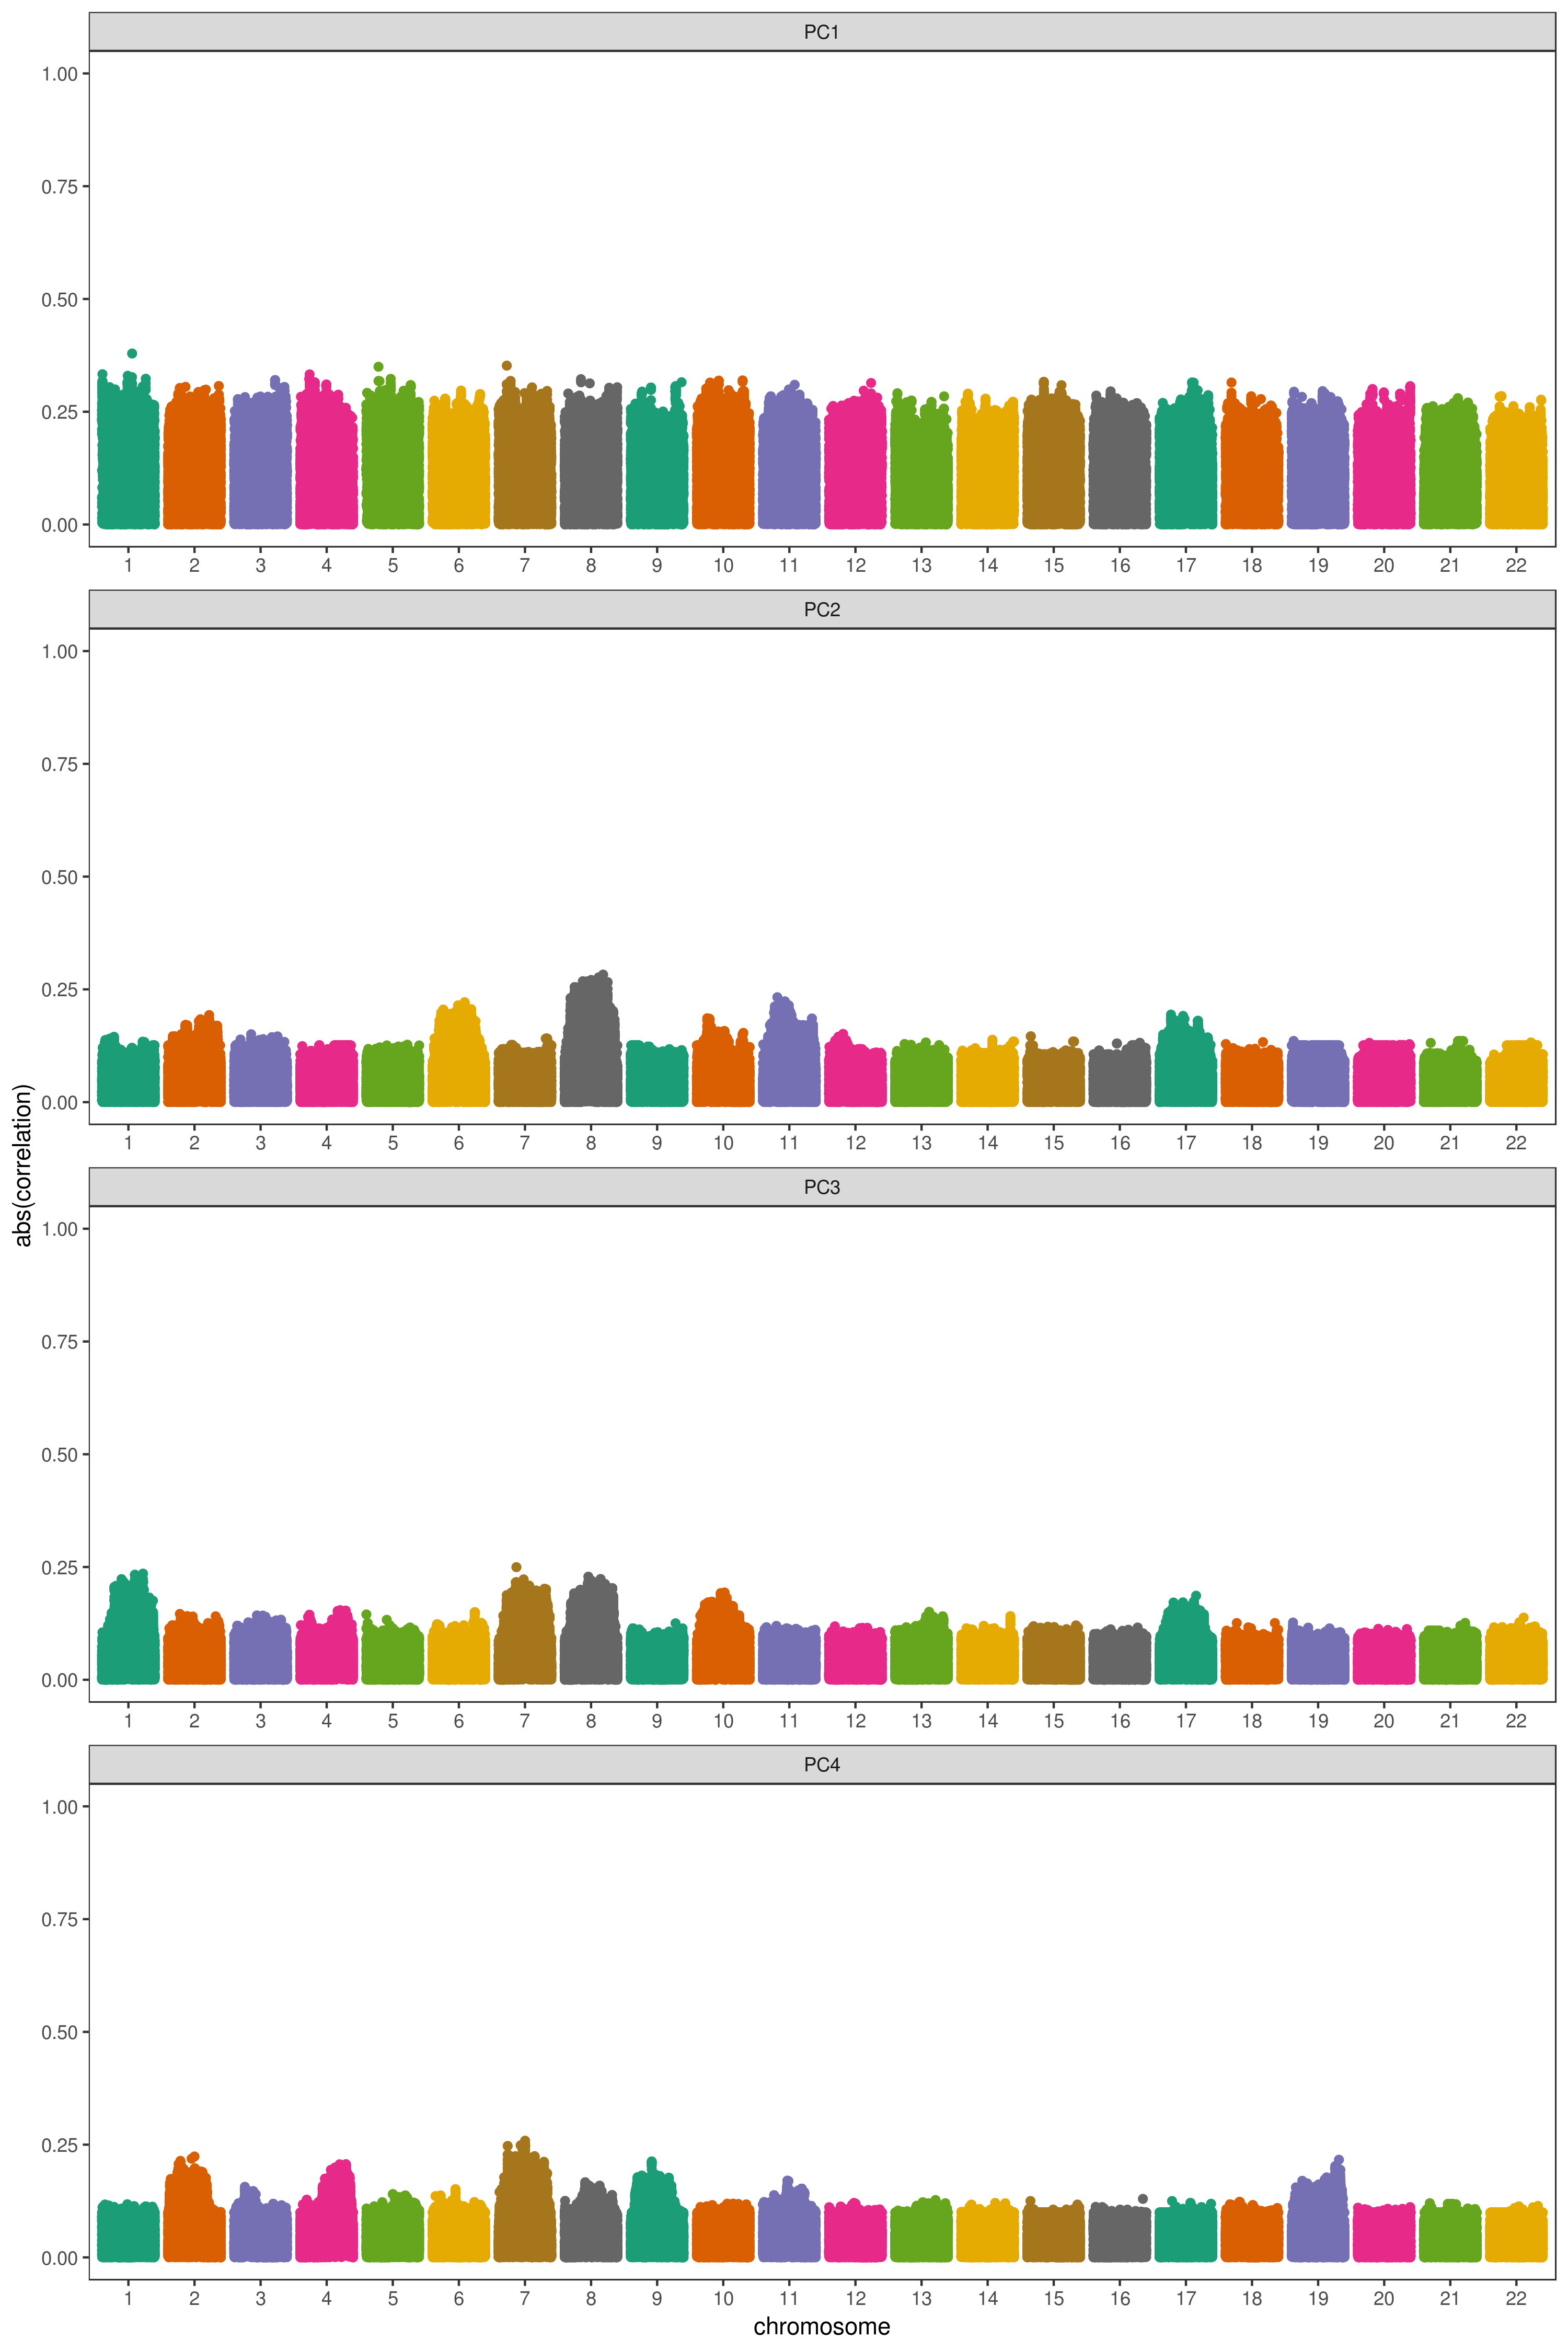
\includegraphics[width=0.24\paperwidth]{figs/JHS_prune_TRUE_0.2_0.5_0.01_snprelate_corr_1}
%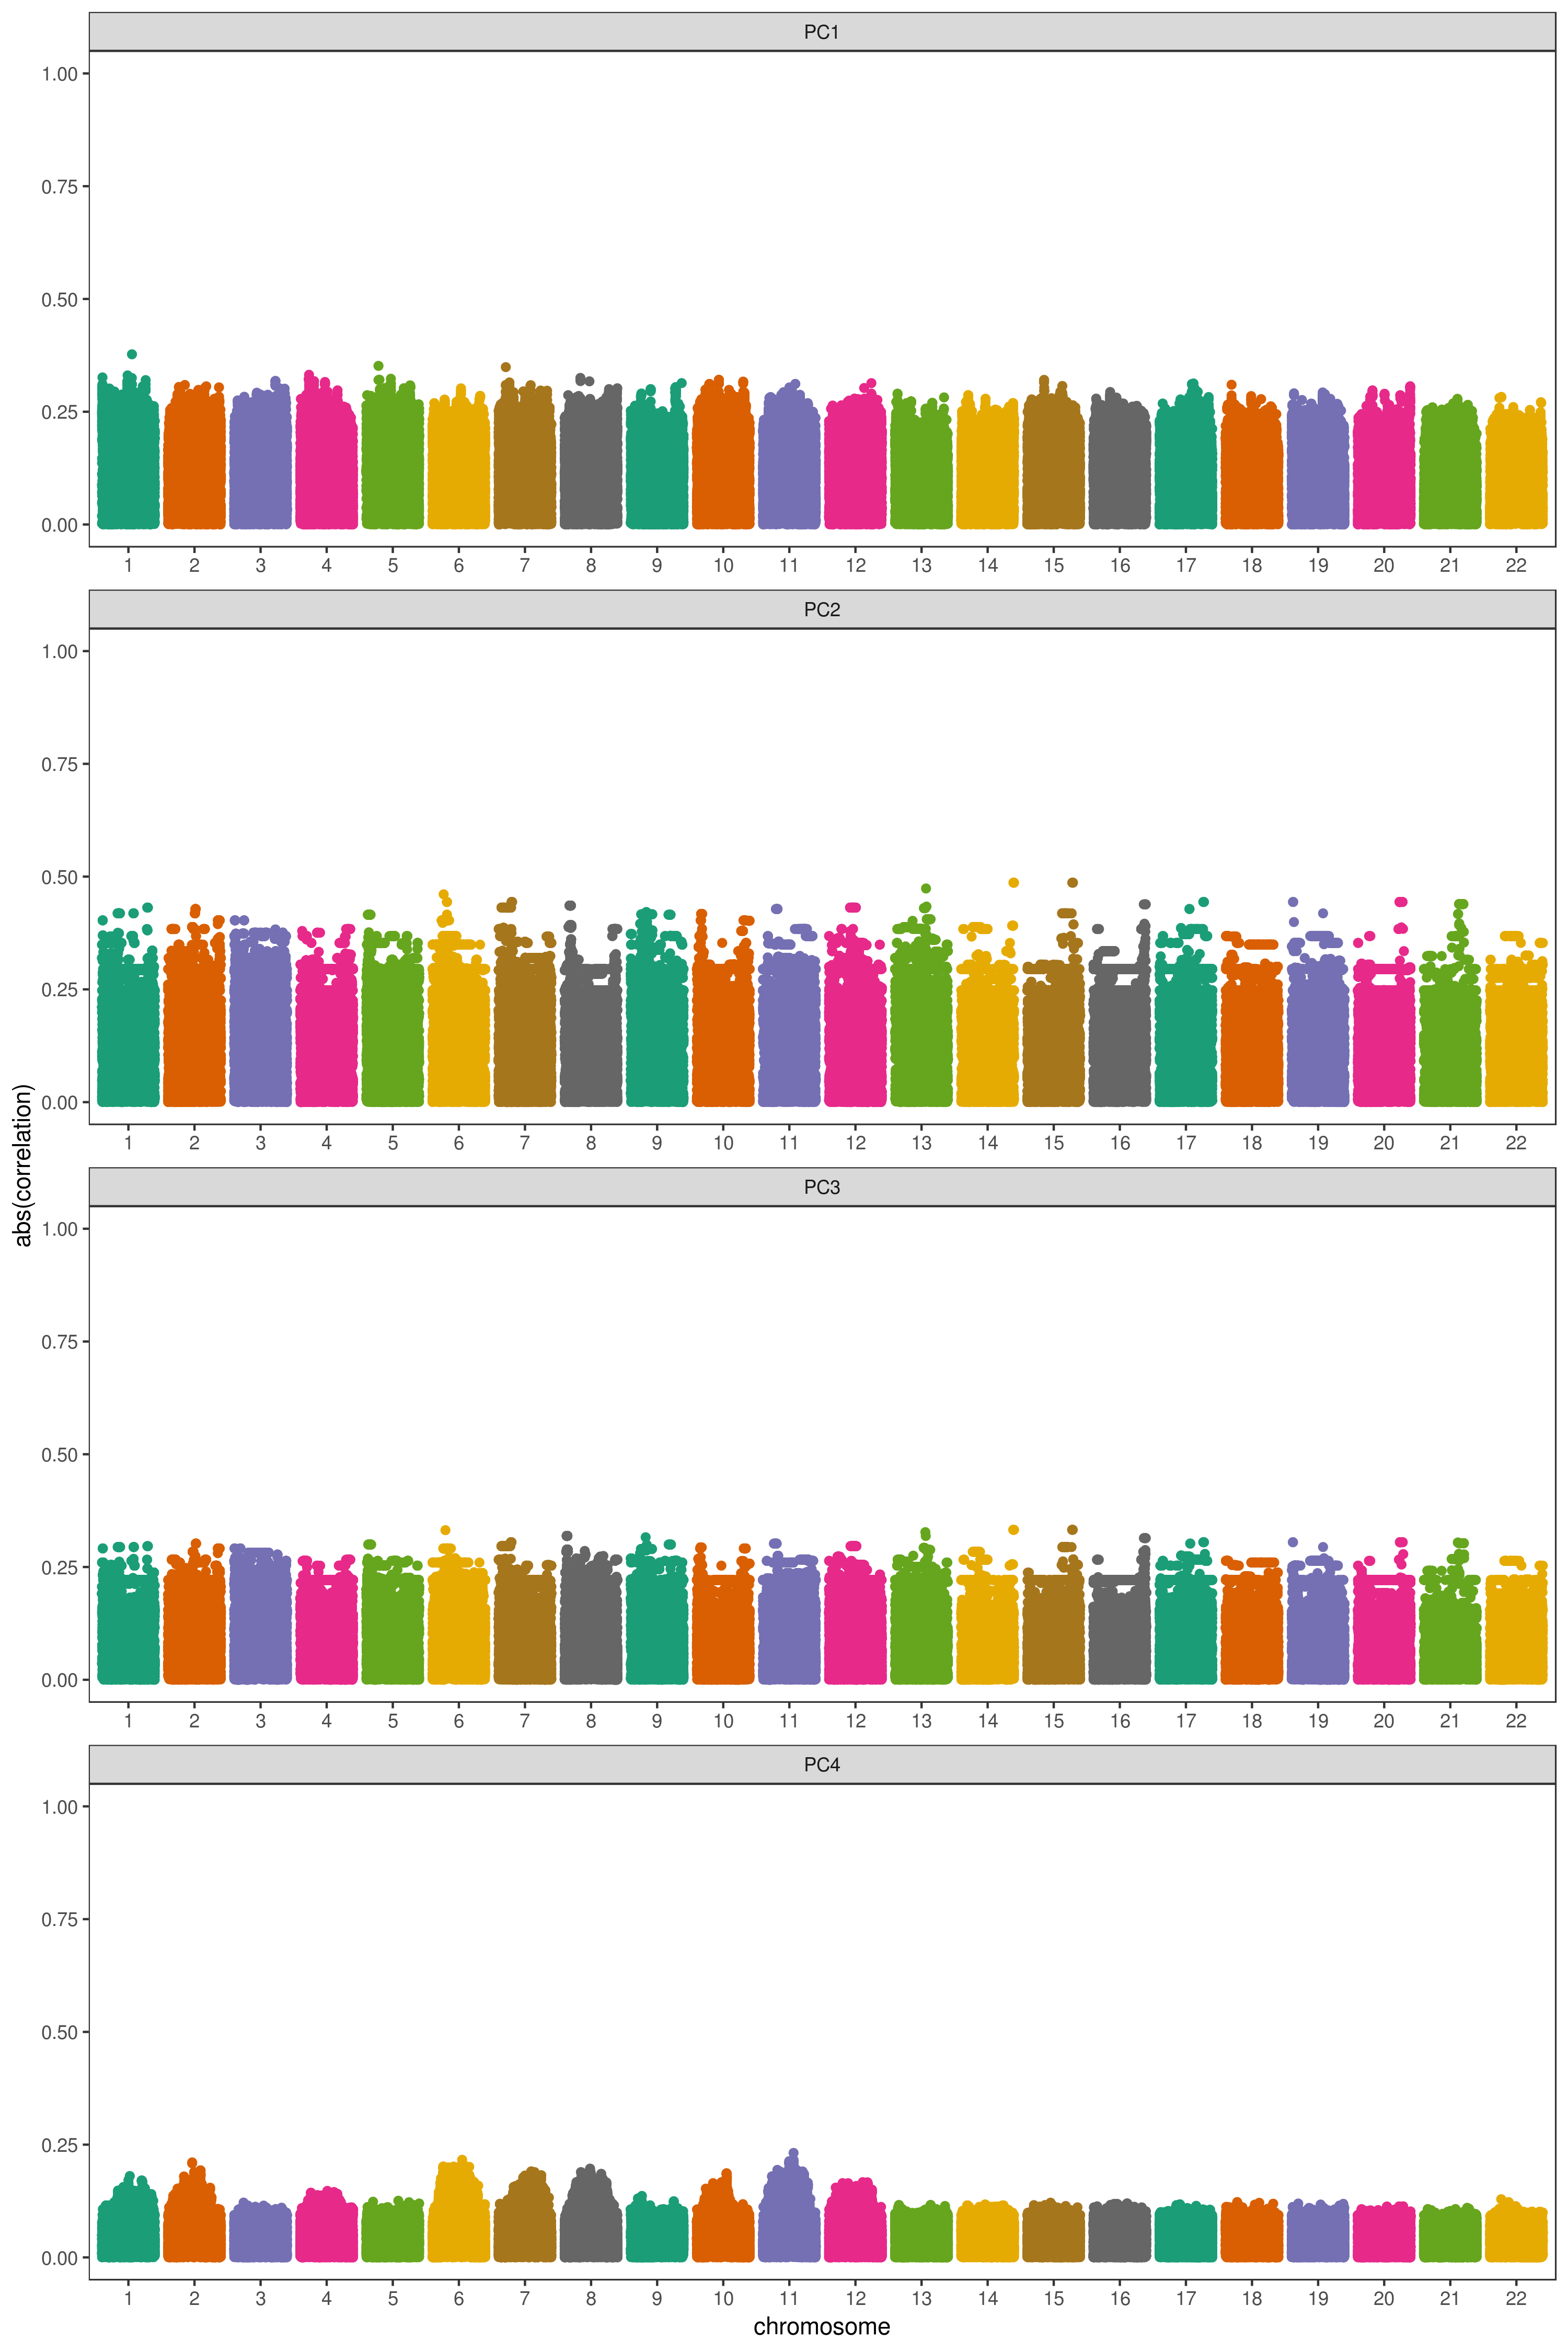
\includegraphics[width=0.24\paperwidth]{figs/JHS_prune_TRUE_0.1_0.5_0.01_snprelate_corr_1}
%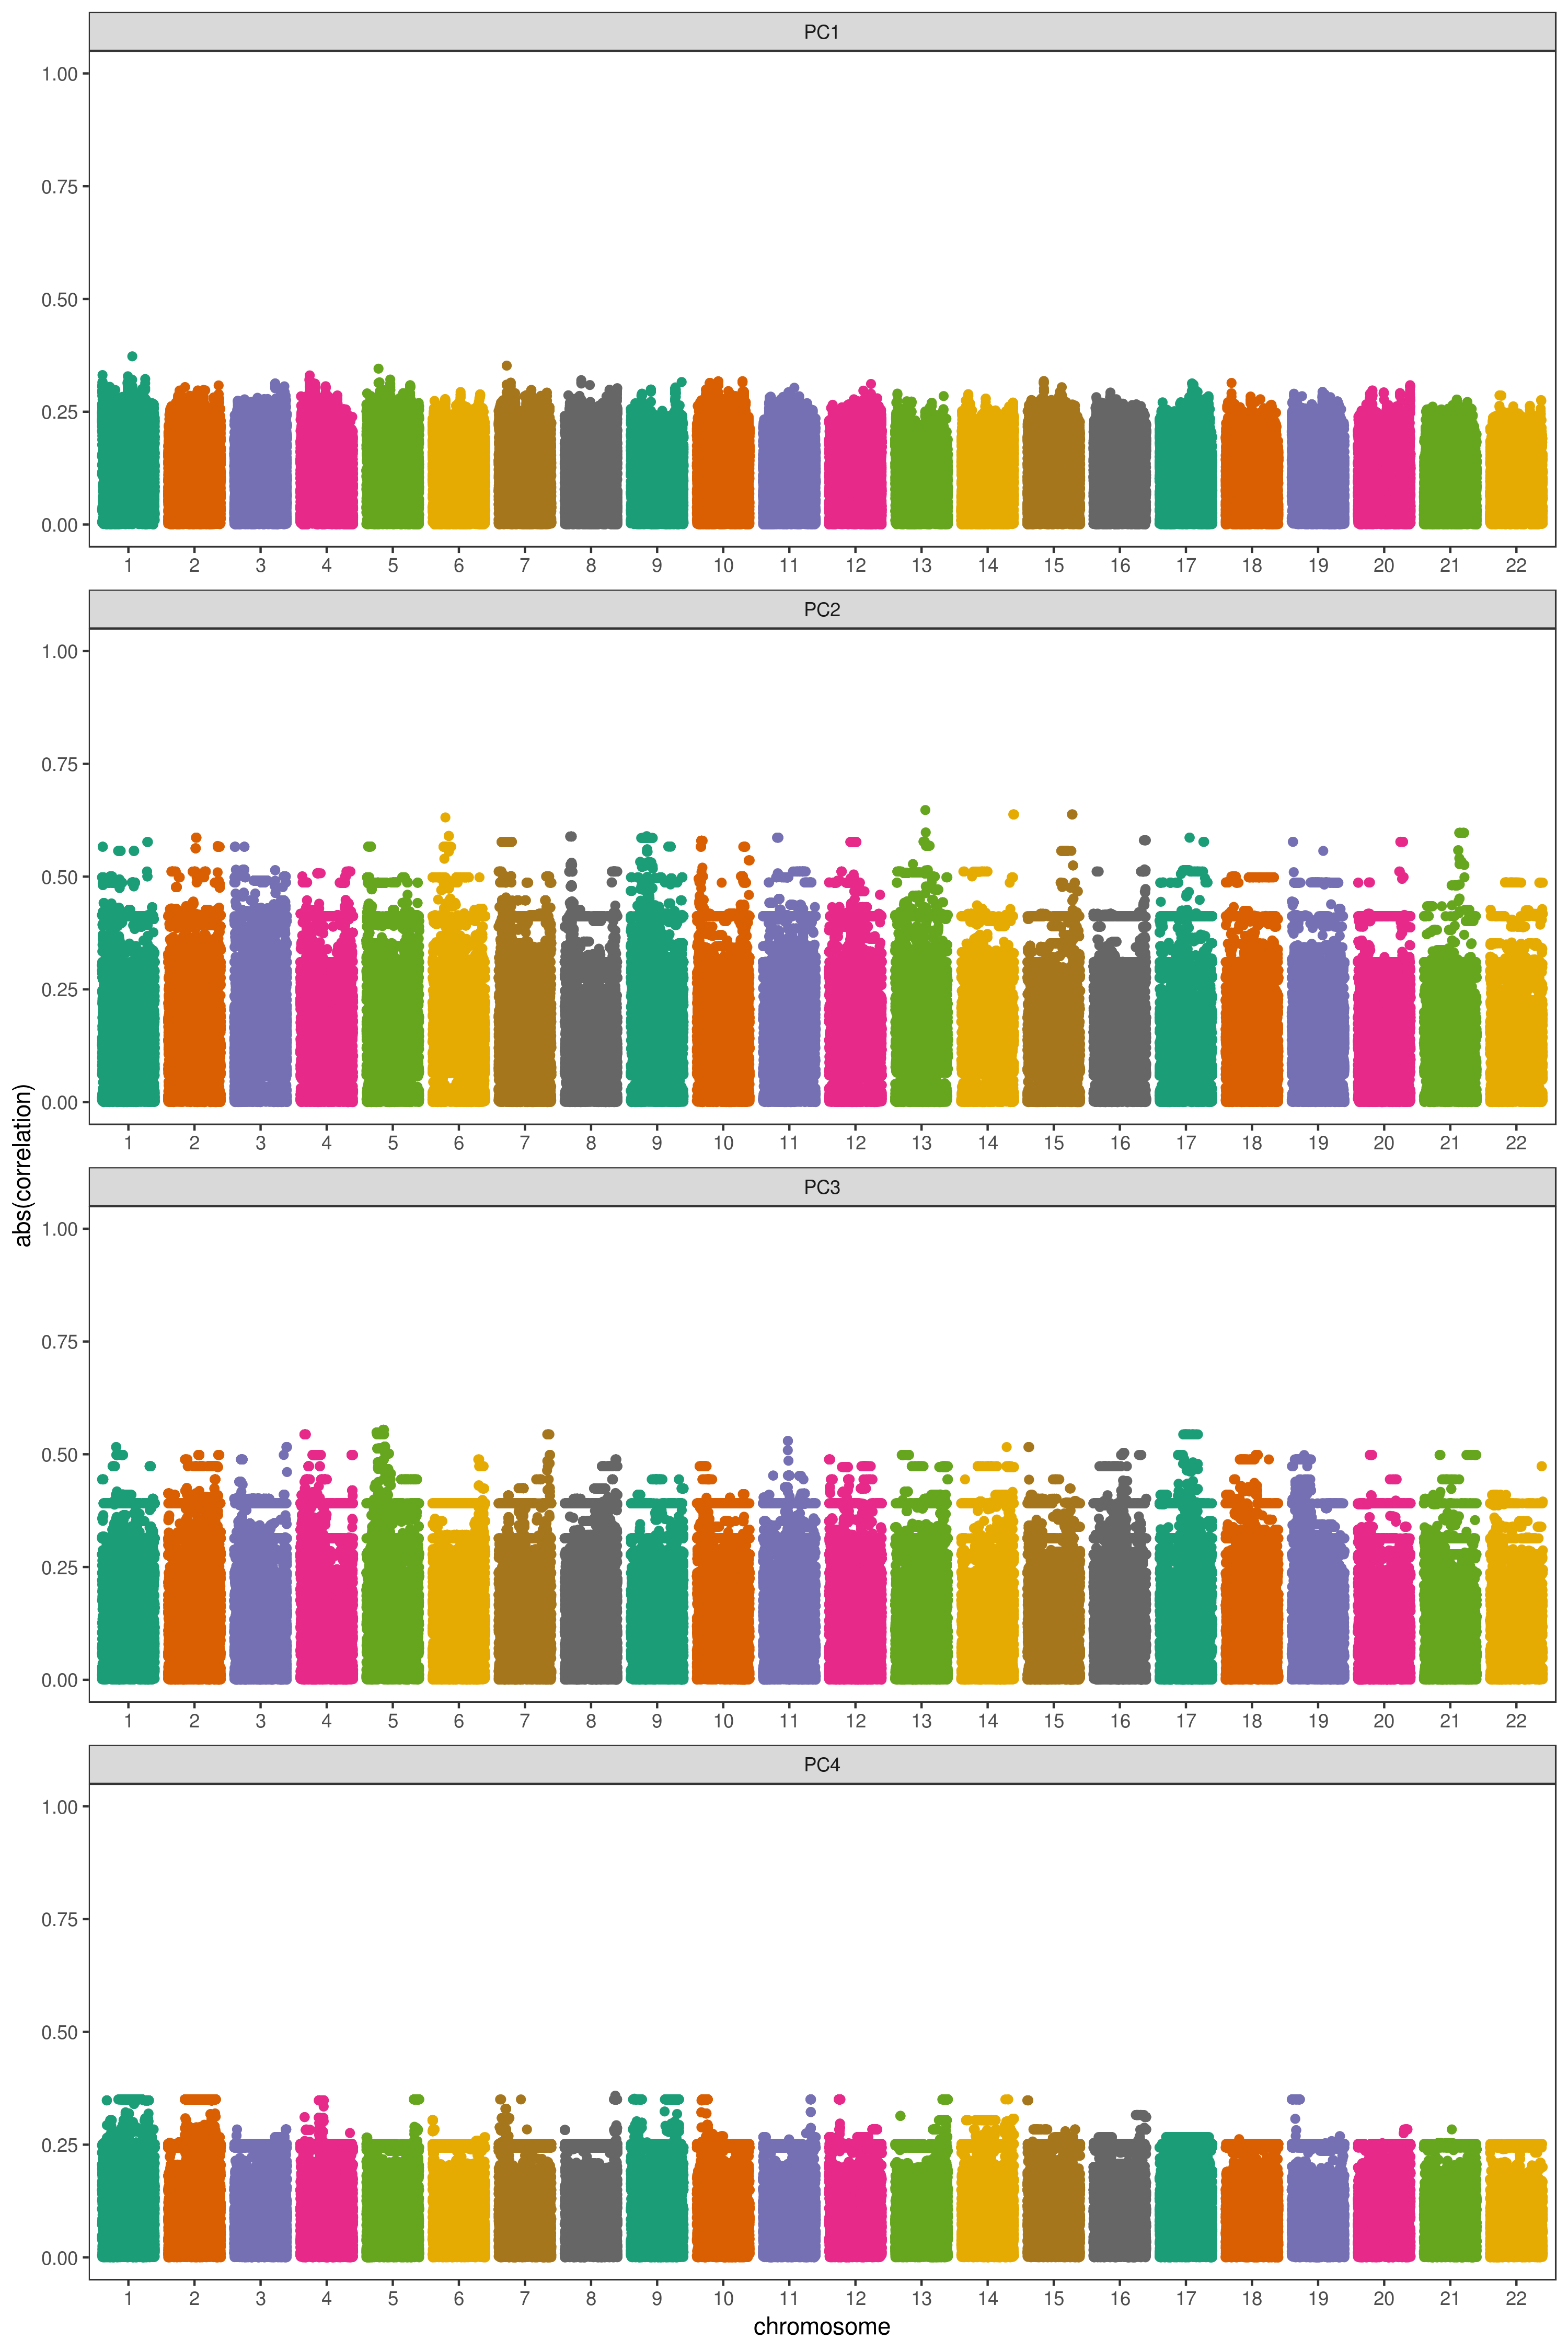
\includegraphics[width=0.24\paperwidth]{figs/JHS_prune_TRUE_0.1_10_0.01_snprelate_corr_1}
%}
%\caption{Correlation between the first four principal components and genotypes in Jackson Heart Study African Americans when previously-identified high-LD regions (Table \ref{tab:highLD}) \textit{are} removed prior to analysis. From left to right, panels correspond to increasingly strict levels of LD pruning: no LD pruning, LD pruning with an $r^2$ threshold of 0.2 and a window size of 0.5 Mb, LD pruning with an $r^2$ threshold of 0.1 and a window size of 0.5 Mb, and LD pruning with an $r^2$ threshold of 0.1 and a window size of 10 Mb.}
%\end{figure}

%\begin{figure}[h]
%\label{fig:corrCOPDNoExclude}
%\makebox[\textwidth][c]{
%\includegraphics[width=0.24\paperwidth]{figs/COPD_prune_FALSE_1_0_0.01_snprelate_corr_1}
%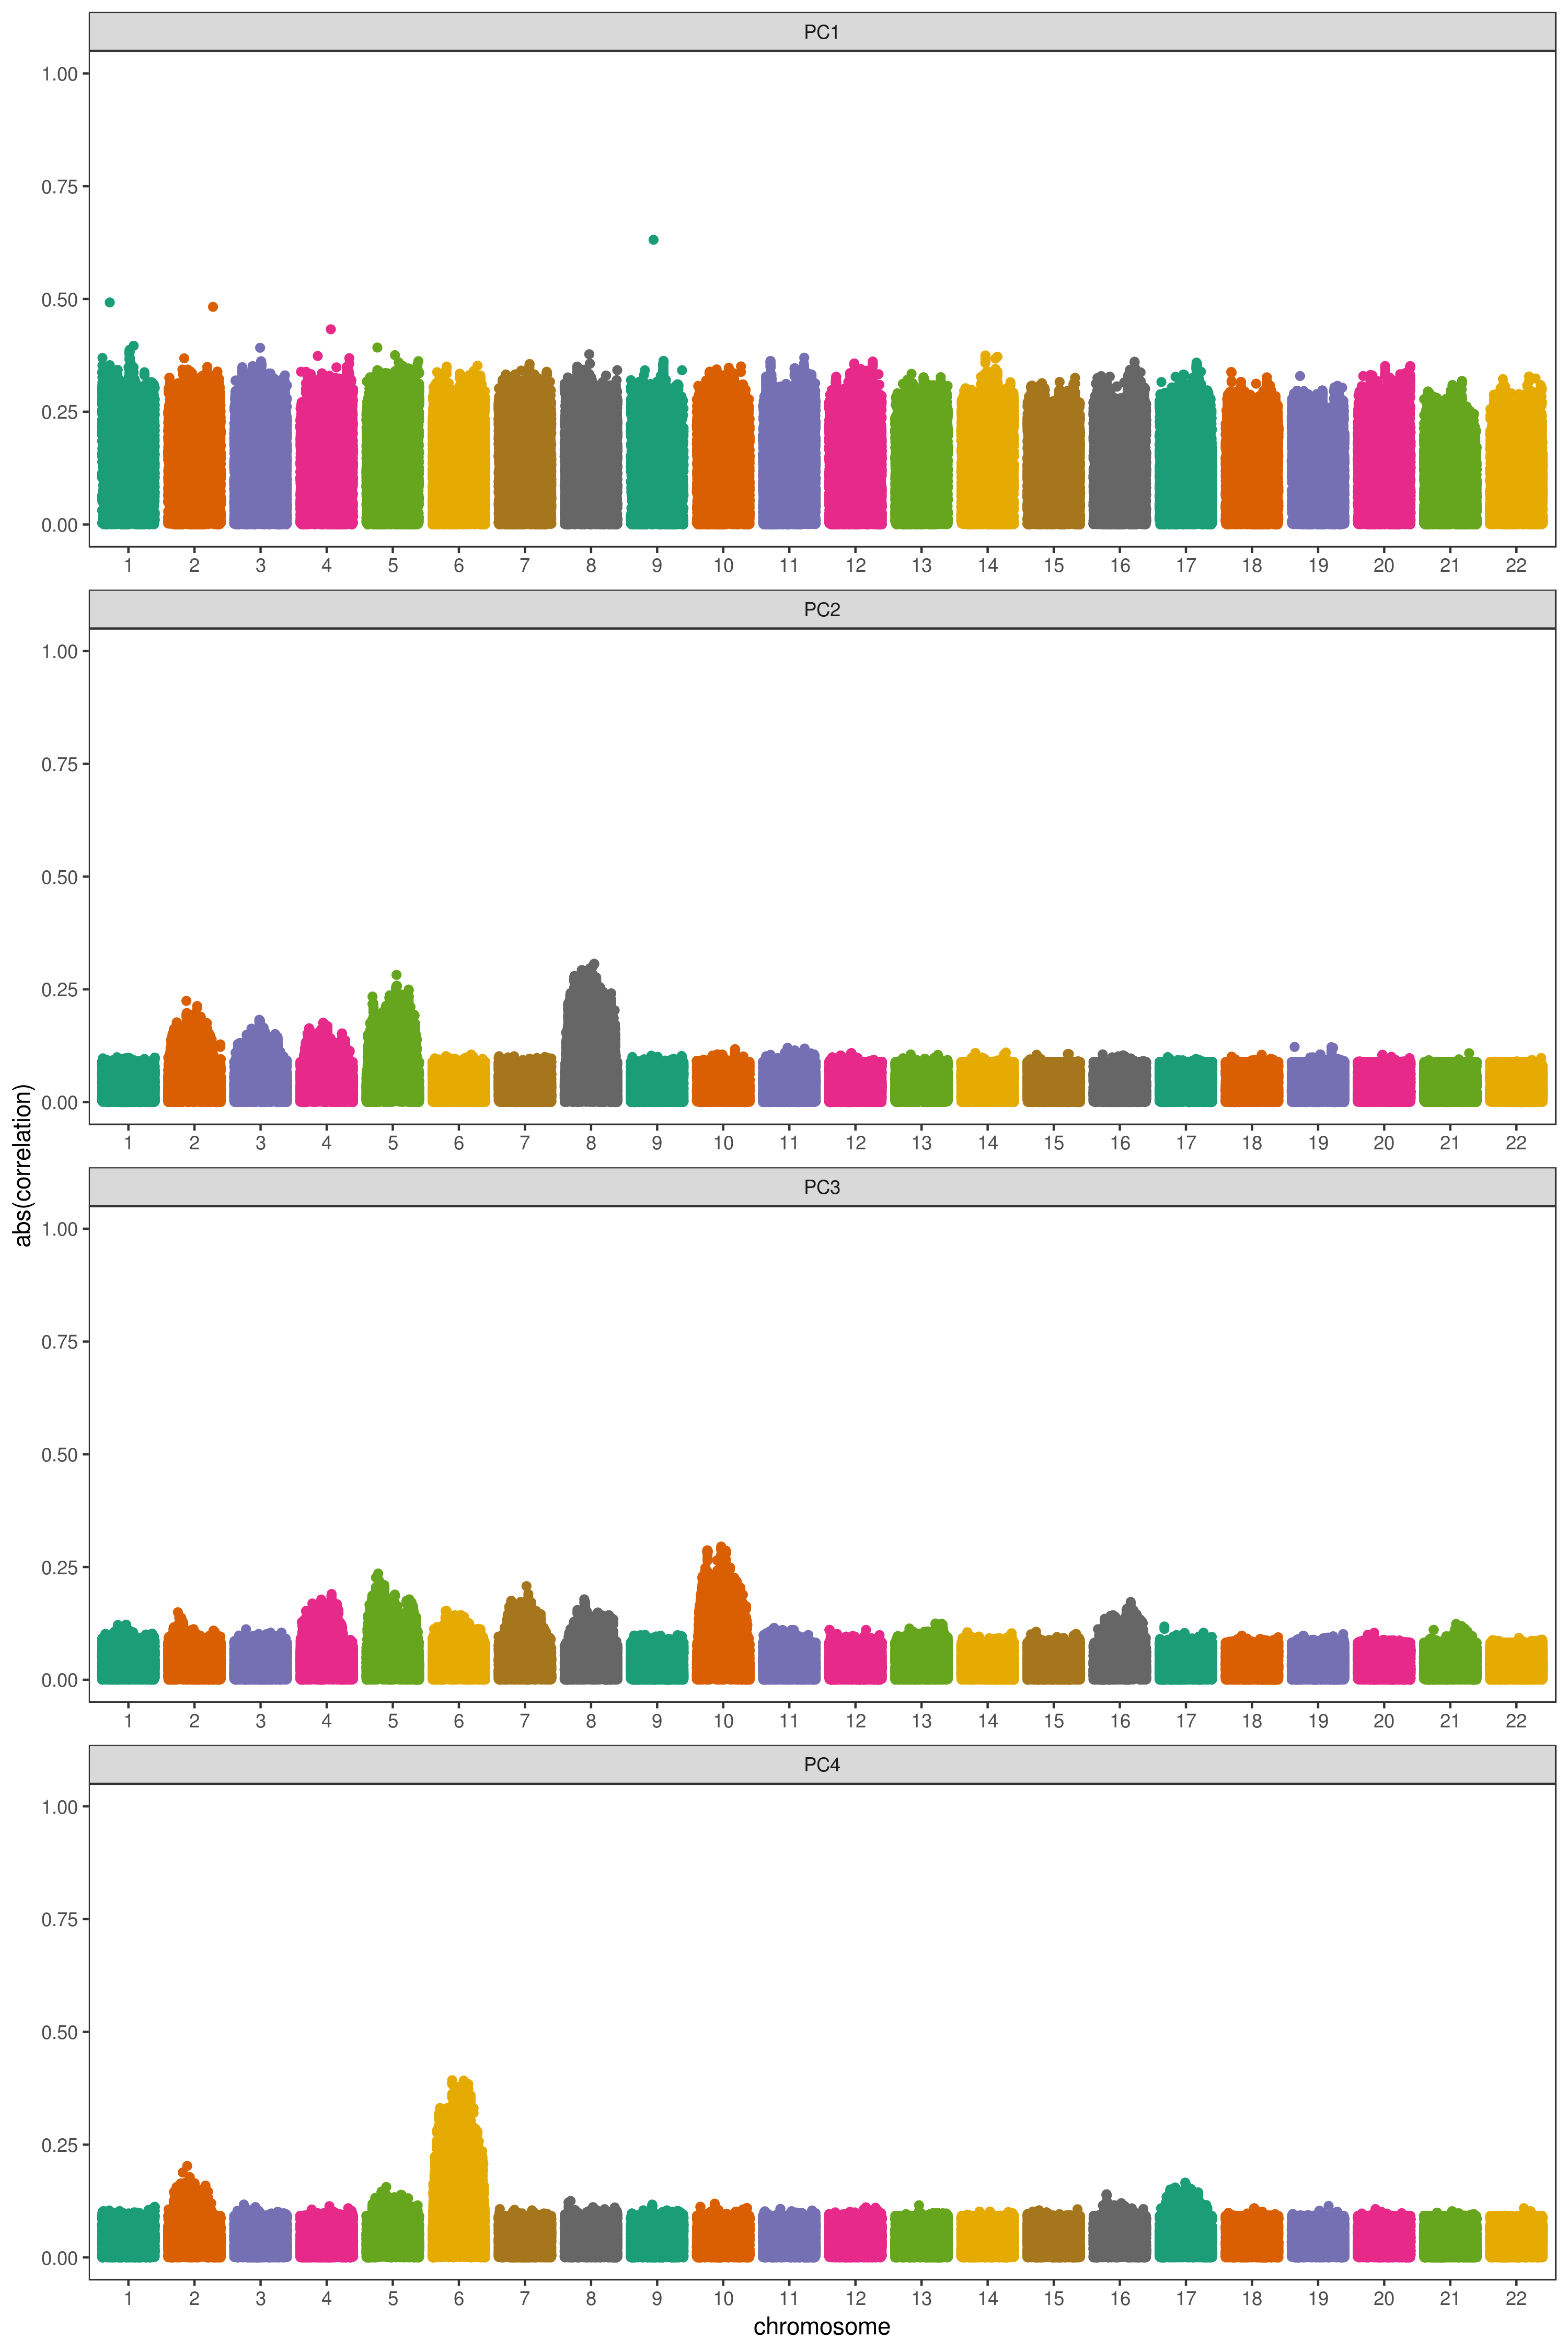
\includegraphics[width=0.24\paperwidth]{figs/COPD_prune_FALSE_0.2_0.5_0.01_snprelate_corr_1}
%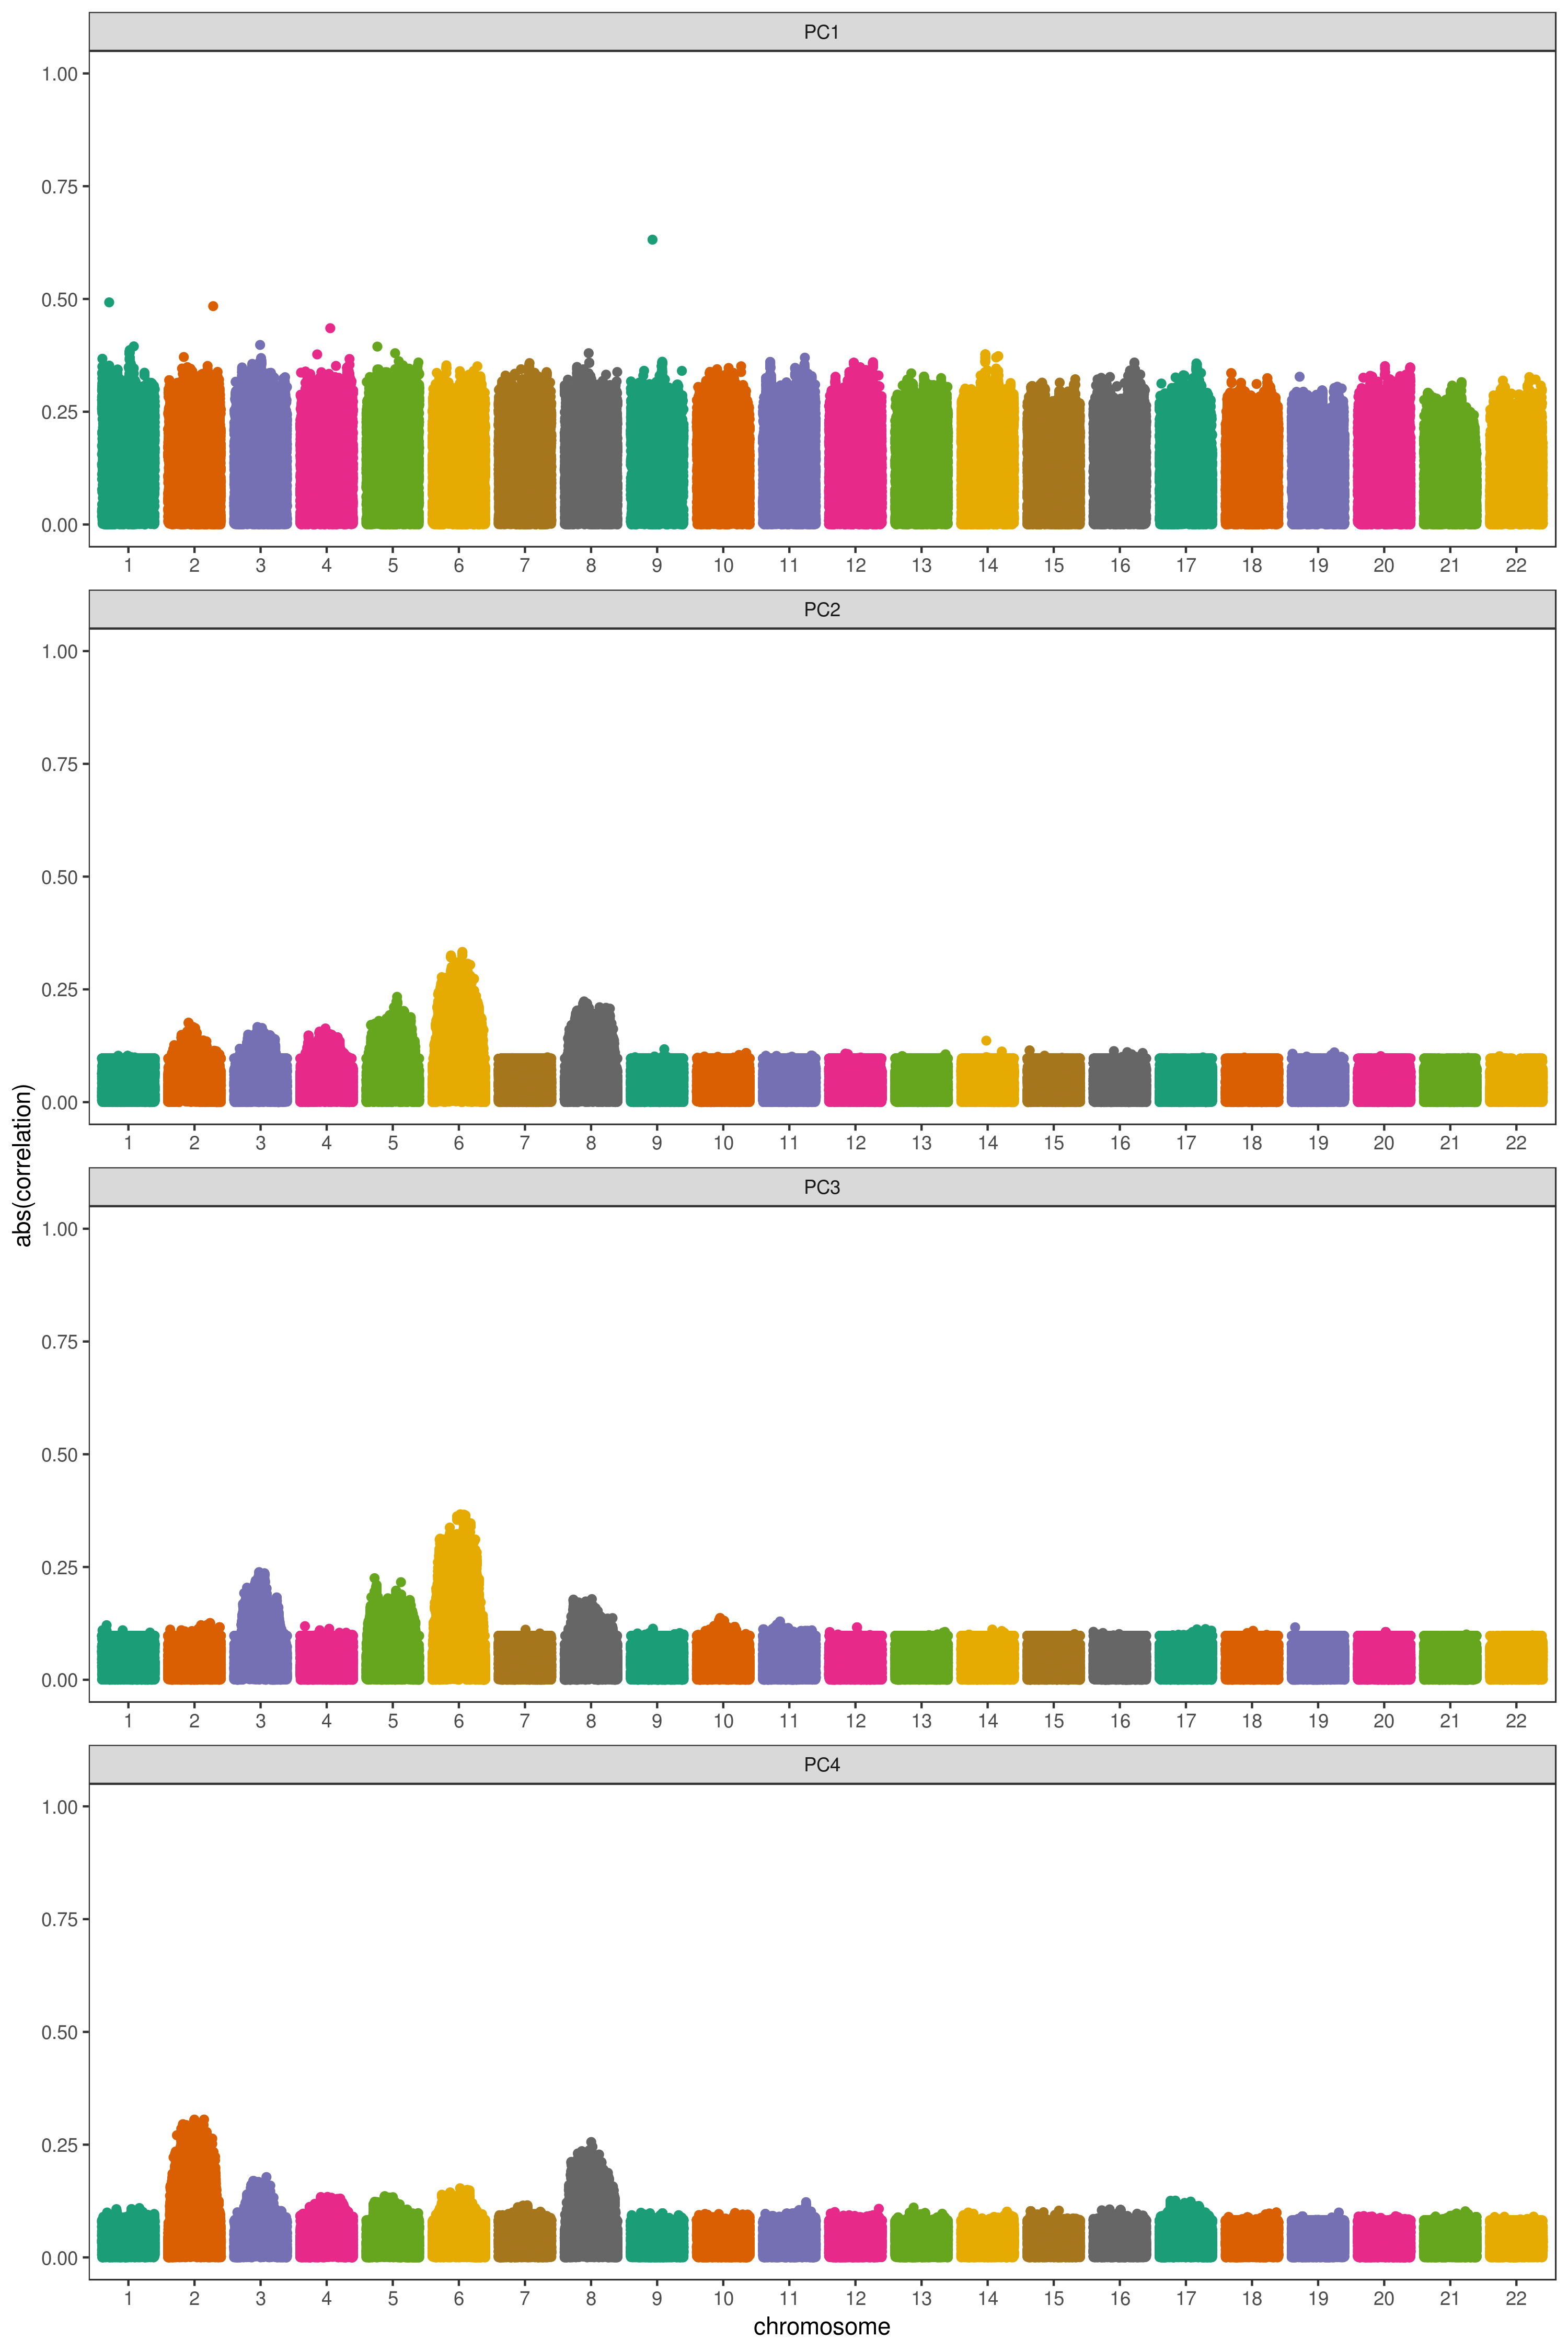
\includegraphics[width=0.24\paperwidth]{figs/COPD_prune_FALSE_0.1_0.5_0.01_snprelate_corr_1}
%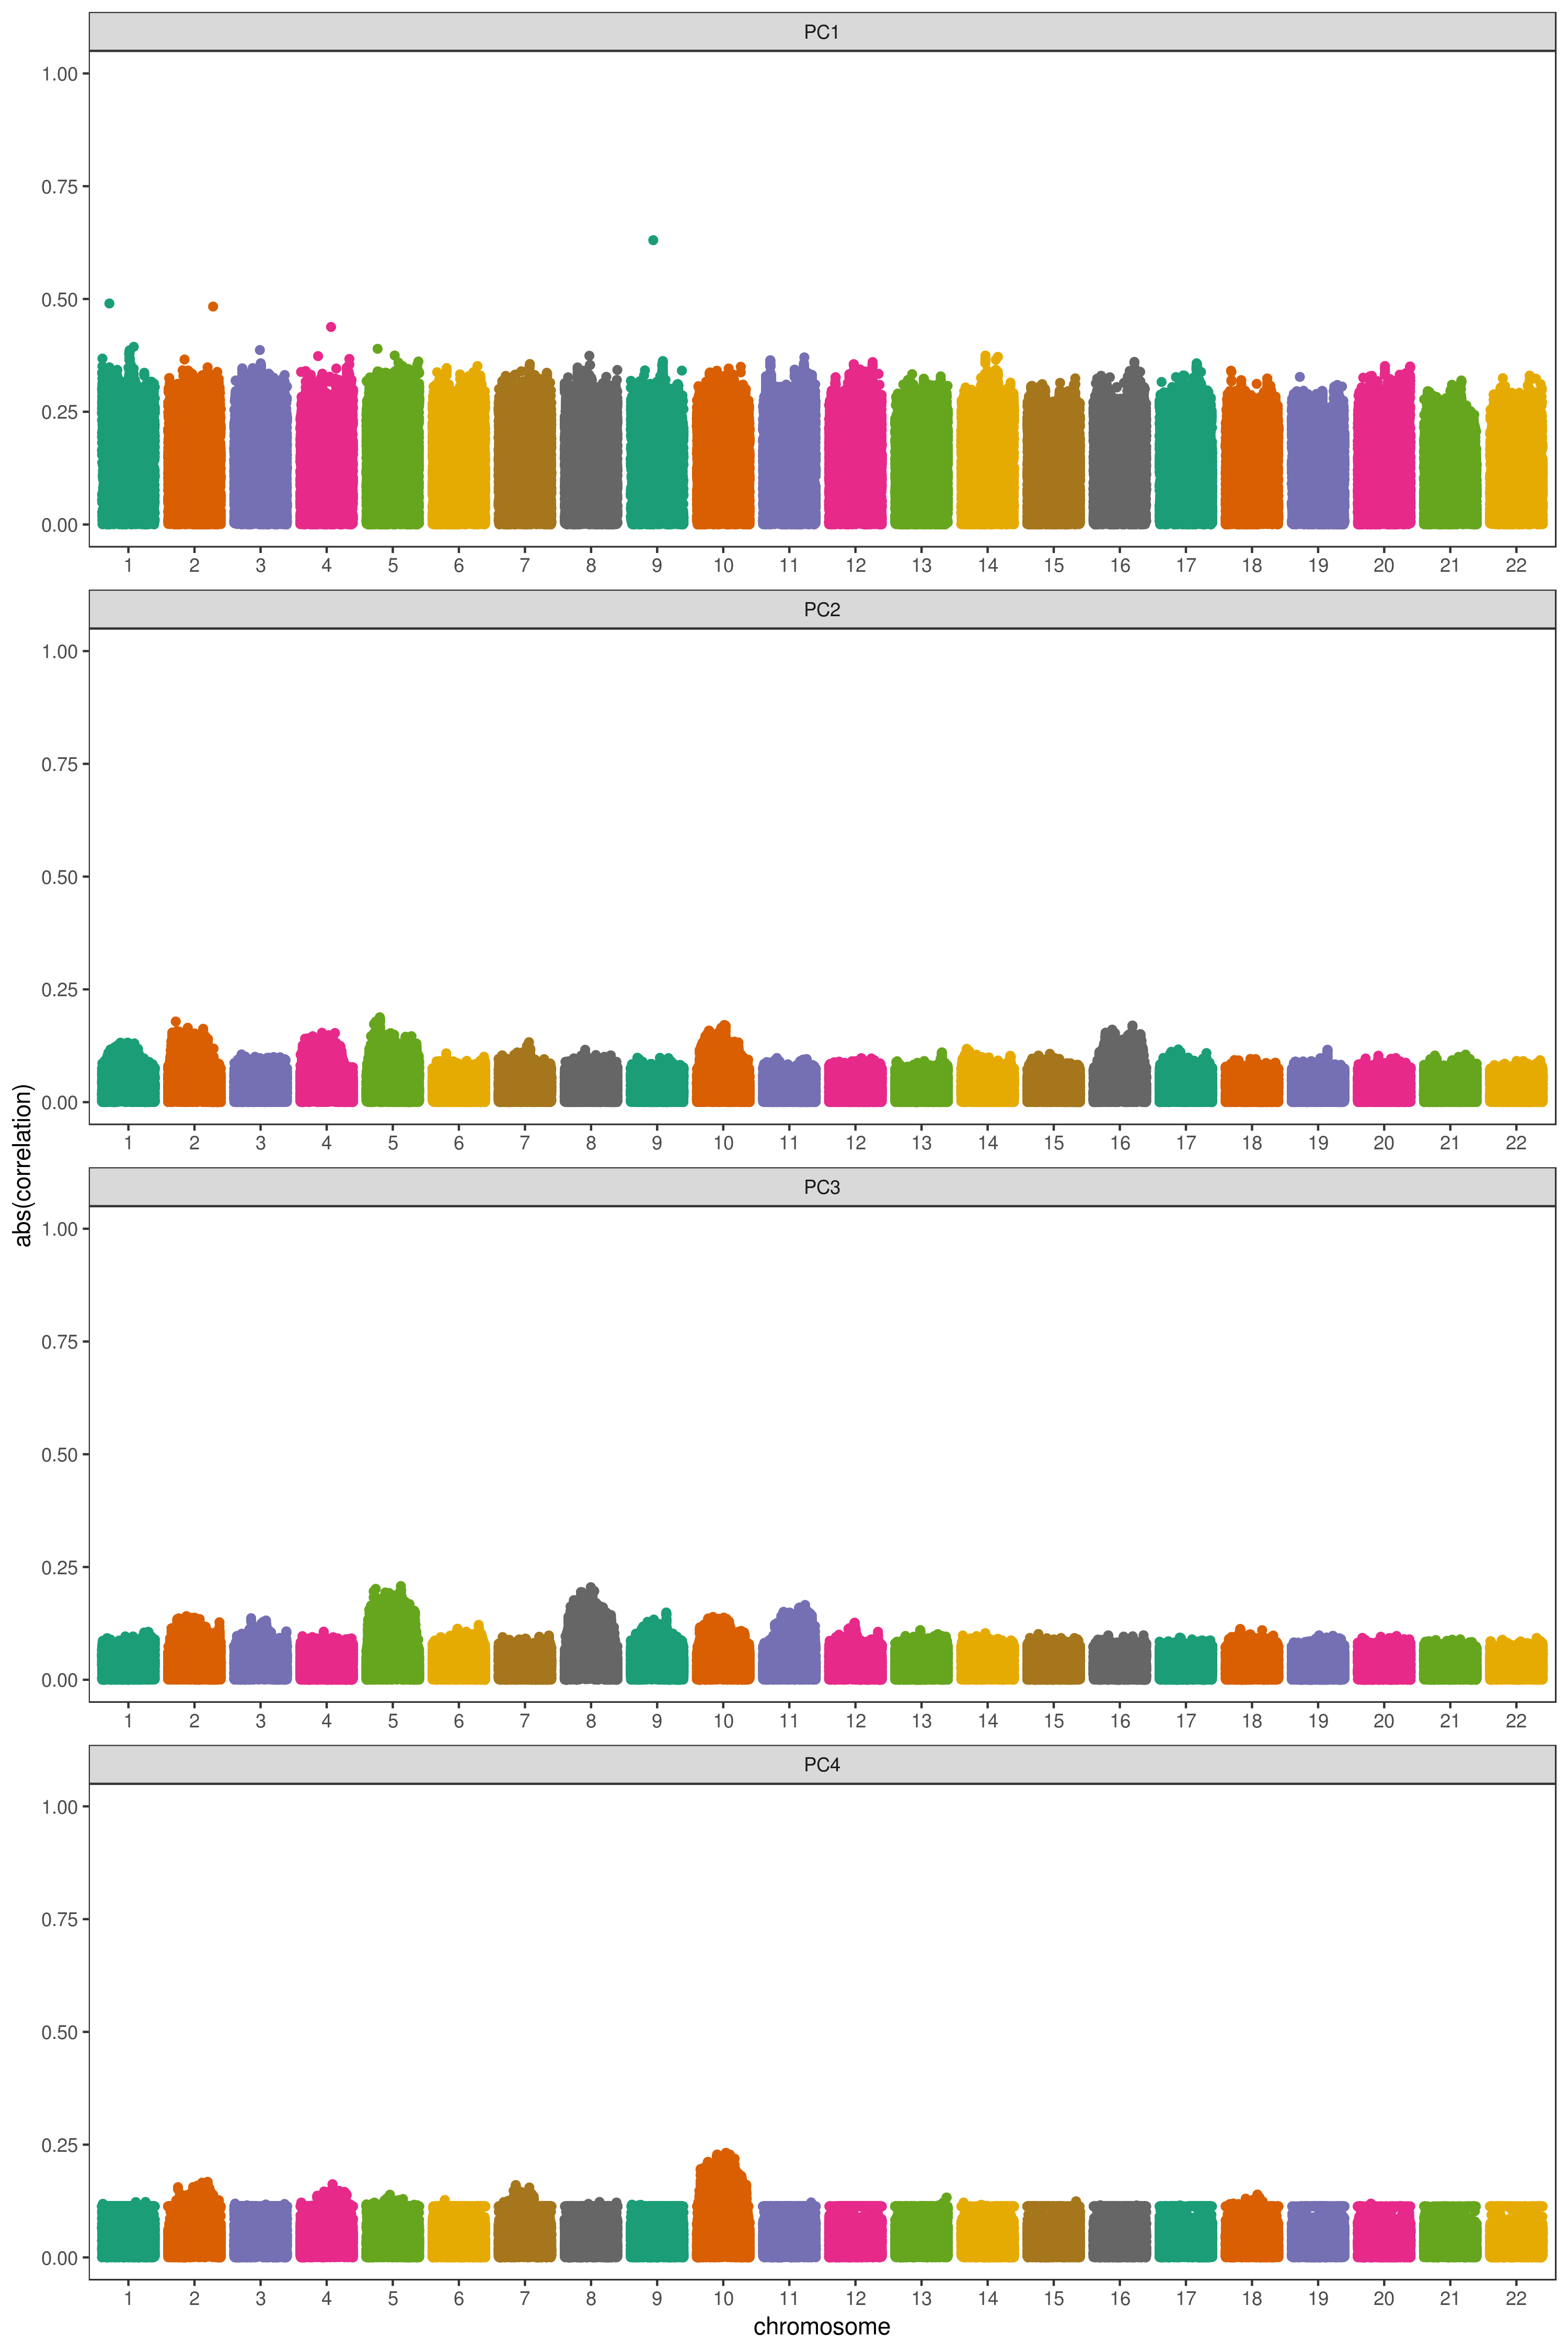
\includegraphics[width=0.24\paperwidth]{figs/COPD_prune_FALSE_0.1_10_0.01_snprelate_corr_1}
%}
%\caption{Correlation between the first four principal components and genotypes in COPDGene African Americans when previously-identified high-LD regions (Table \ref{tab:highLD}) \textit{are not} removed prior to analysis. From left to right, panels correspond to increasingly strict levels of LD pruning: no LD pruning, LD pruning with an $r^2$ threshold of 0.2 and a window size of 0.5 Mb, LD pruning with an $r^2$ threshold of 0.1 and a window size of 0.5 Mb, and LD pruning with an $r^2$ threshold of 0.1 and a window size of 10 Mb.}
%\end{figure}

%\begin{figure}[h]
%\label{fig:corrCOPDExclude}
%\makebox[\textwidth][c]{
%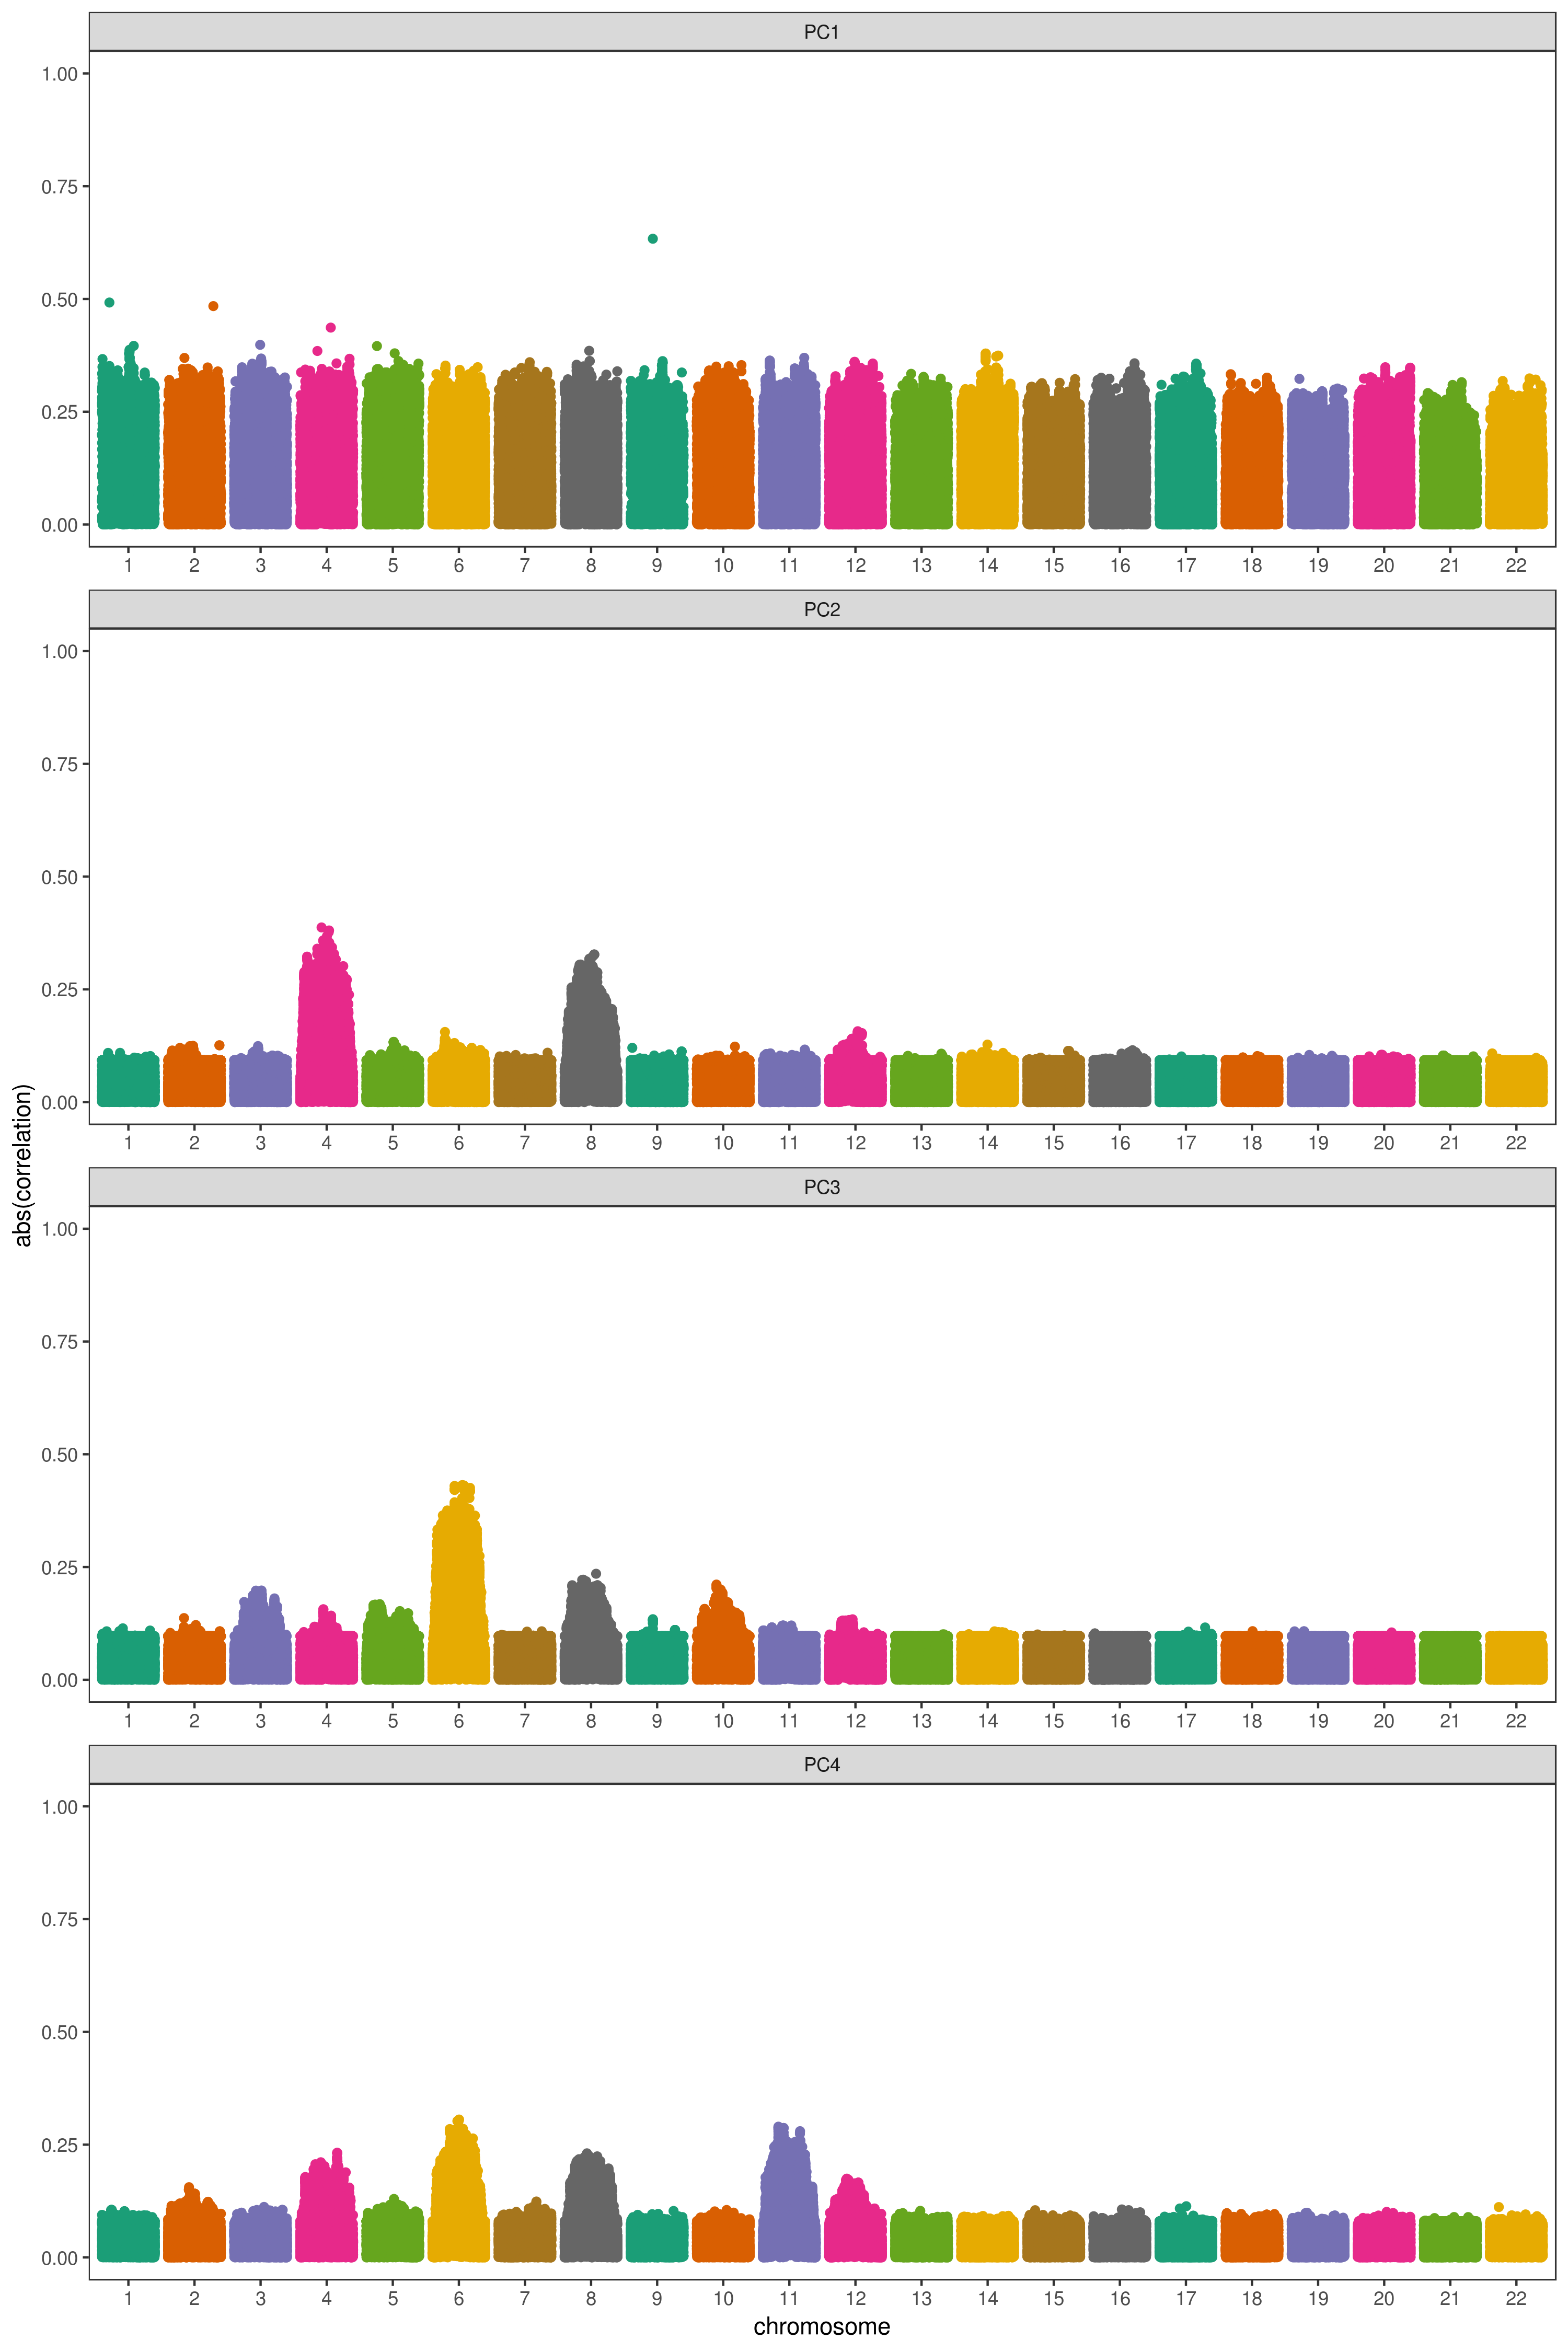
\includegraphics[width=0.24\paperwidth]{figs/COPD_prune_TRUE_1_0_0.01_snprelate_corr_1}
%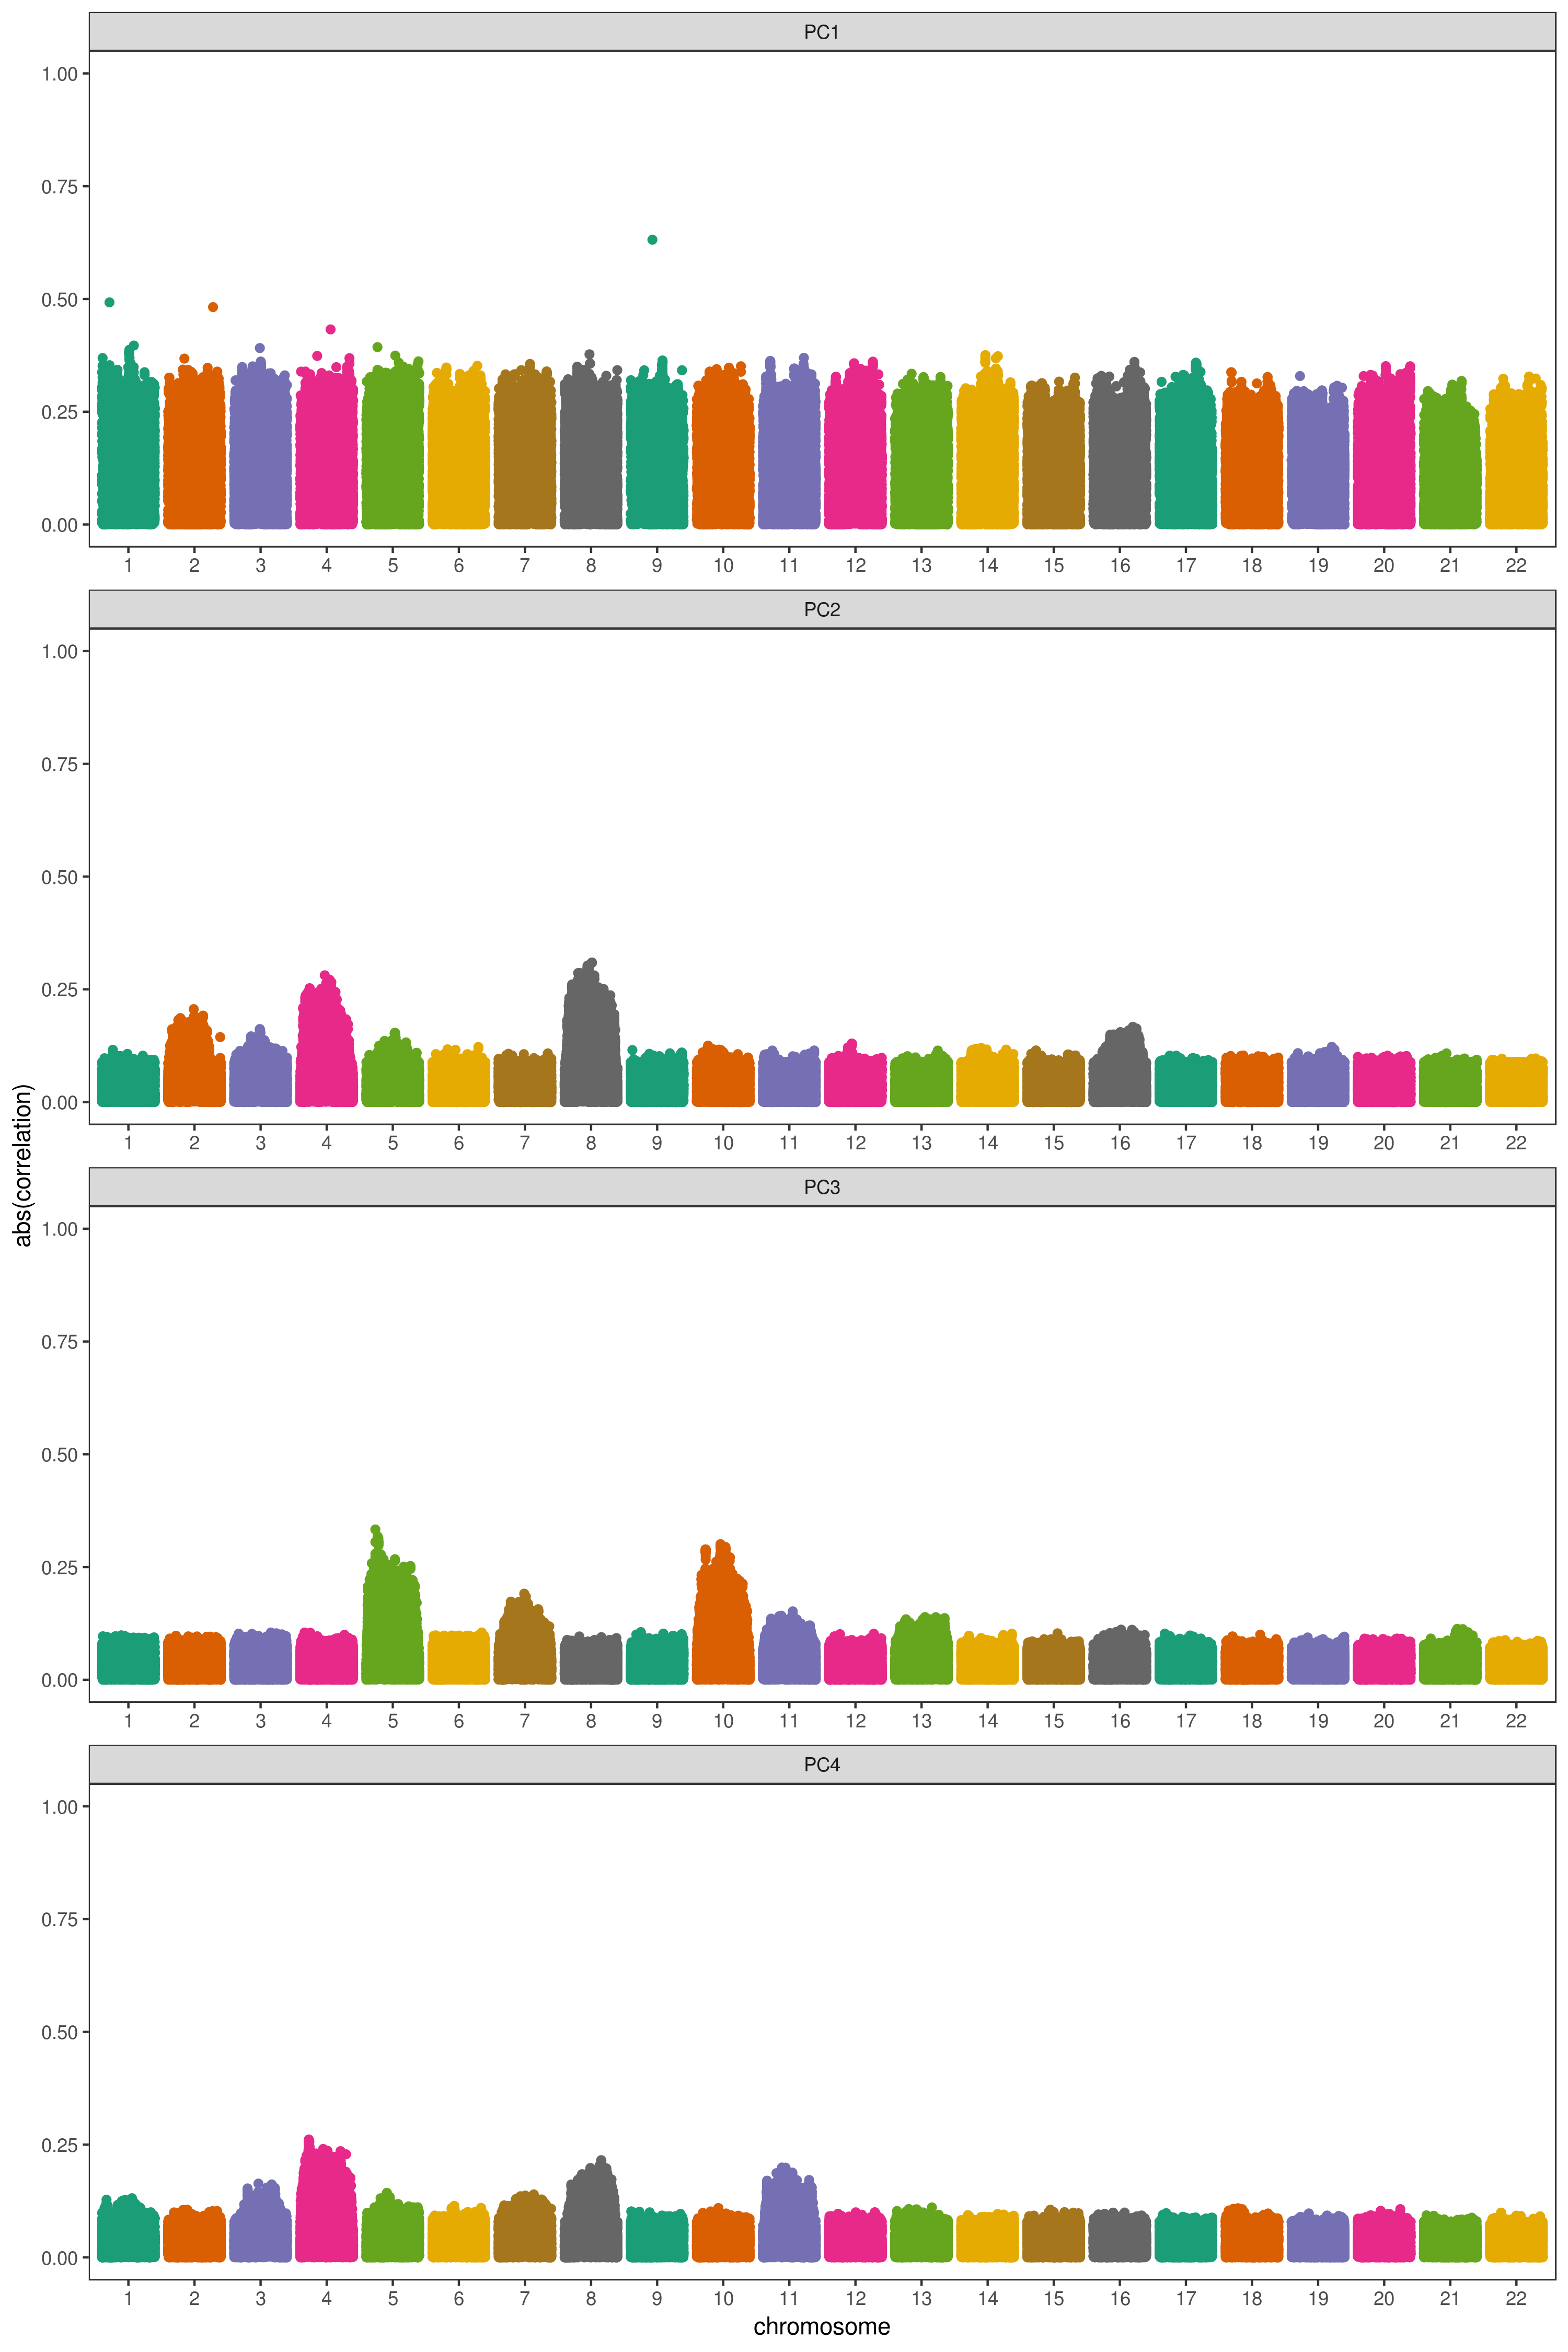
\includegraphics[width=0.24\paperwidth]{figs/COPD_prune_TRUE_0.2_0.5_0.01_snprelate_corr_1}
%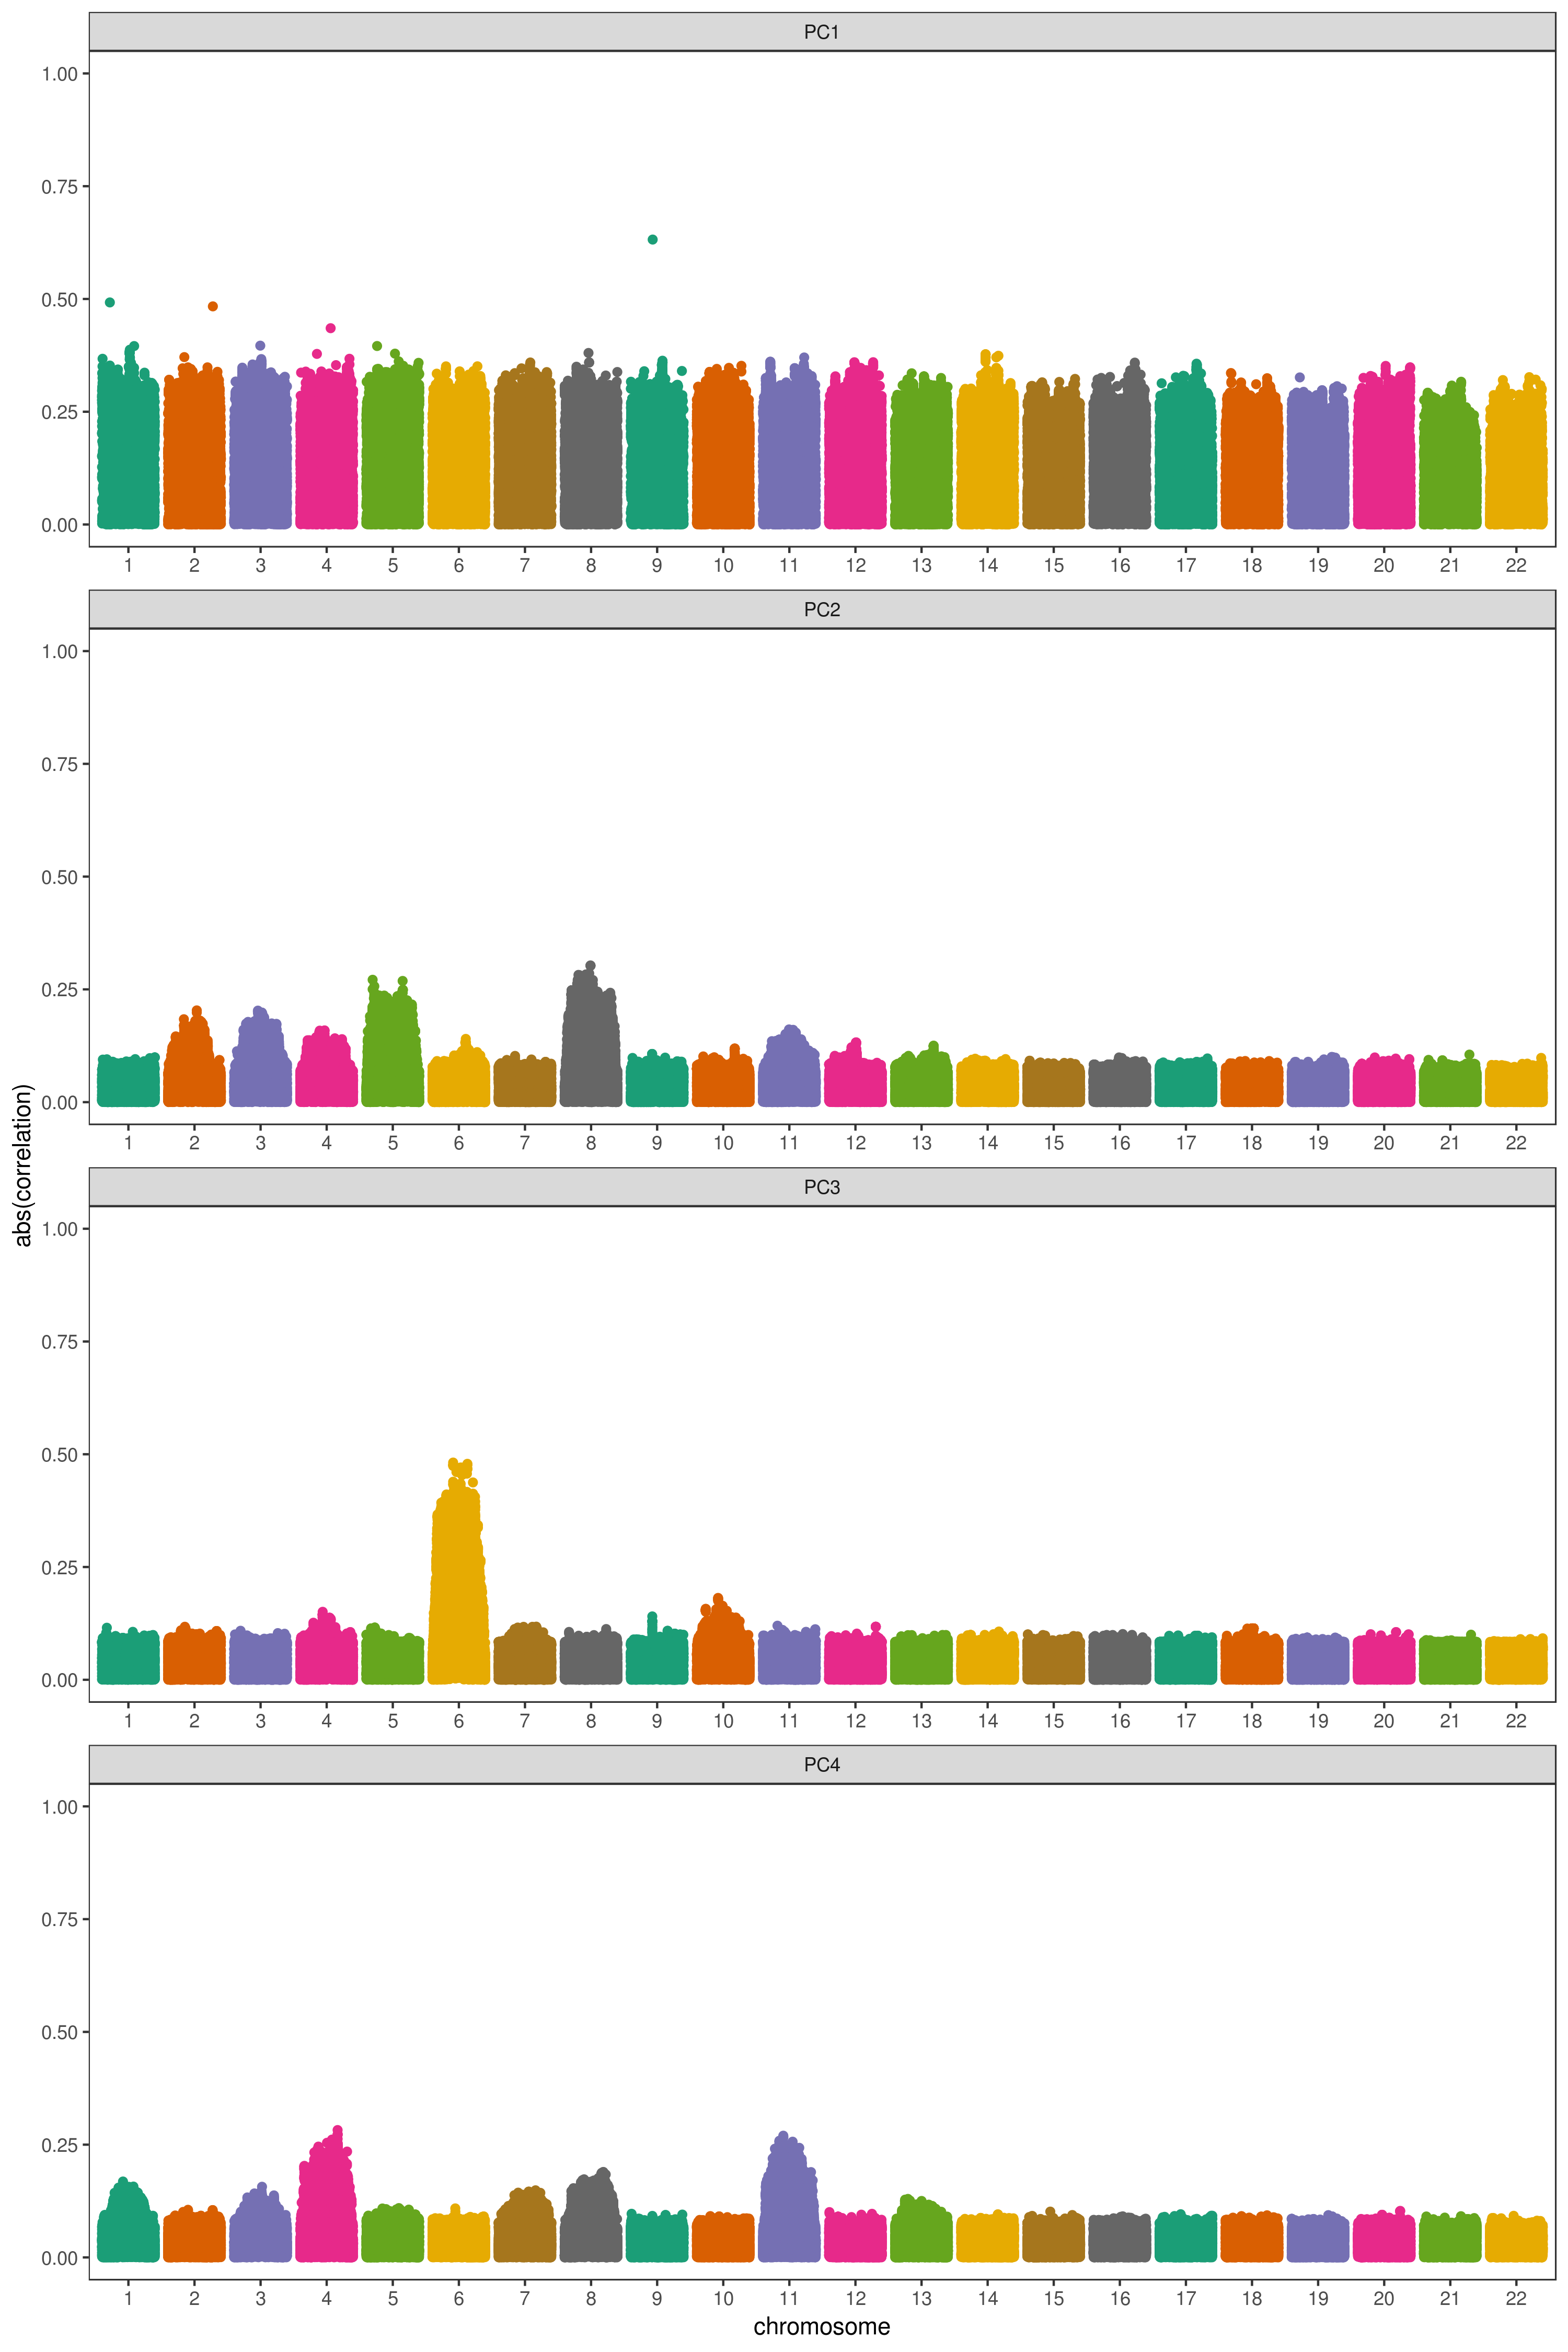
\includegraphics[width=0.24\paperwidth]{figs/COPD_prune_TRUE_0.1_0.5_0.01_snprelate_corr_1}
%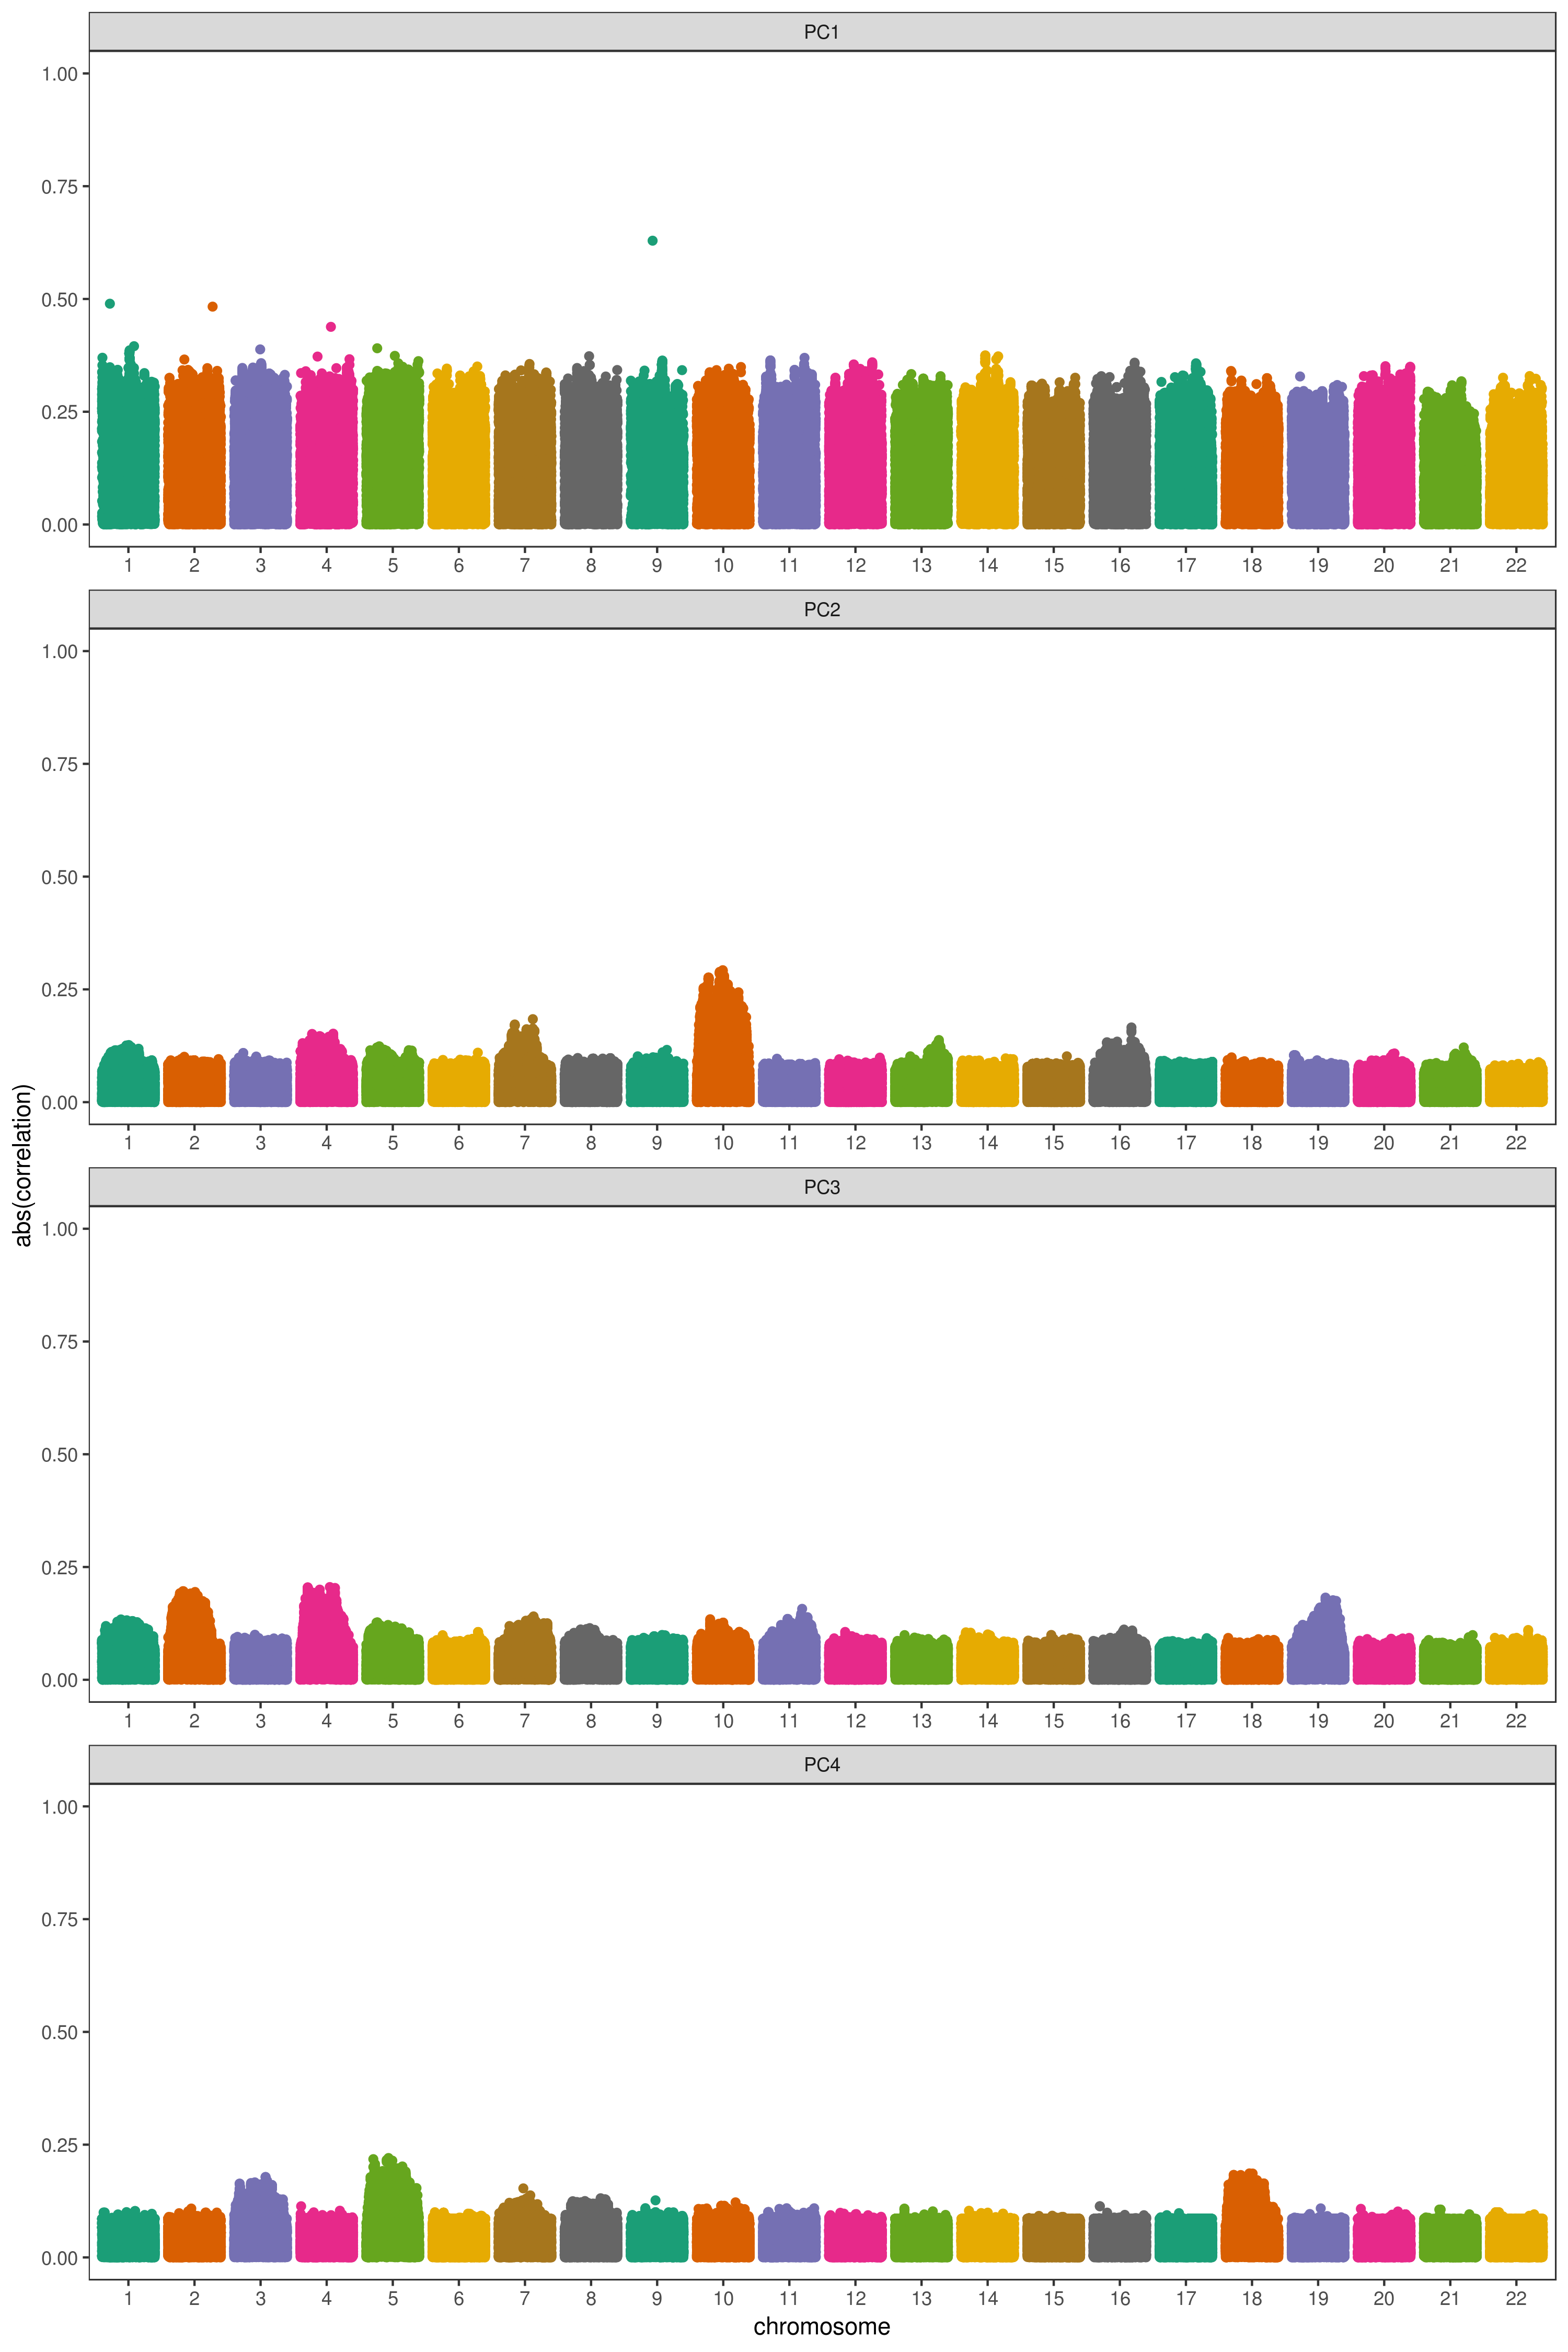
\includegraphics[width=0.24\paperwidth]{figs/COPD_prune_TRUE_0.1_10_0.01_snprelate_corr_1}
%}
%\caption{Correlation between the first four principal components and genotypes in COPDGene African Americans when previously-identified high-LD regions (Table \ref{tab:highLD}) \textit{are} removed prior to analysis. From left to right, panels correspond to increasingly strict levels of LD pruning: no LD pruning, LD pruning with an $r^2$ threshold of 0.2 and a window size of 0.5 Mb, LD pruning with an $r^2$ threshold of 0.1 and a window size of 0.5 Mb, and LD pruning with an $r^2$ threshold of 0.1 and a window size of 10 Mb.}
%\end{figure}


%\begin{figure}
%\label{fig:corrEuropeans}
%\makebox[\textwidth][c]{
%\includegraphics[width=0.32\paperwidth]{figs/EUR_prune_FALSE_1_0_0.01_snprelate_load_1}
%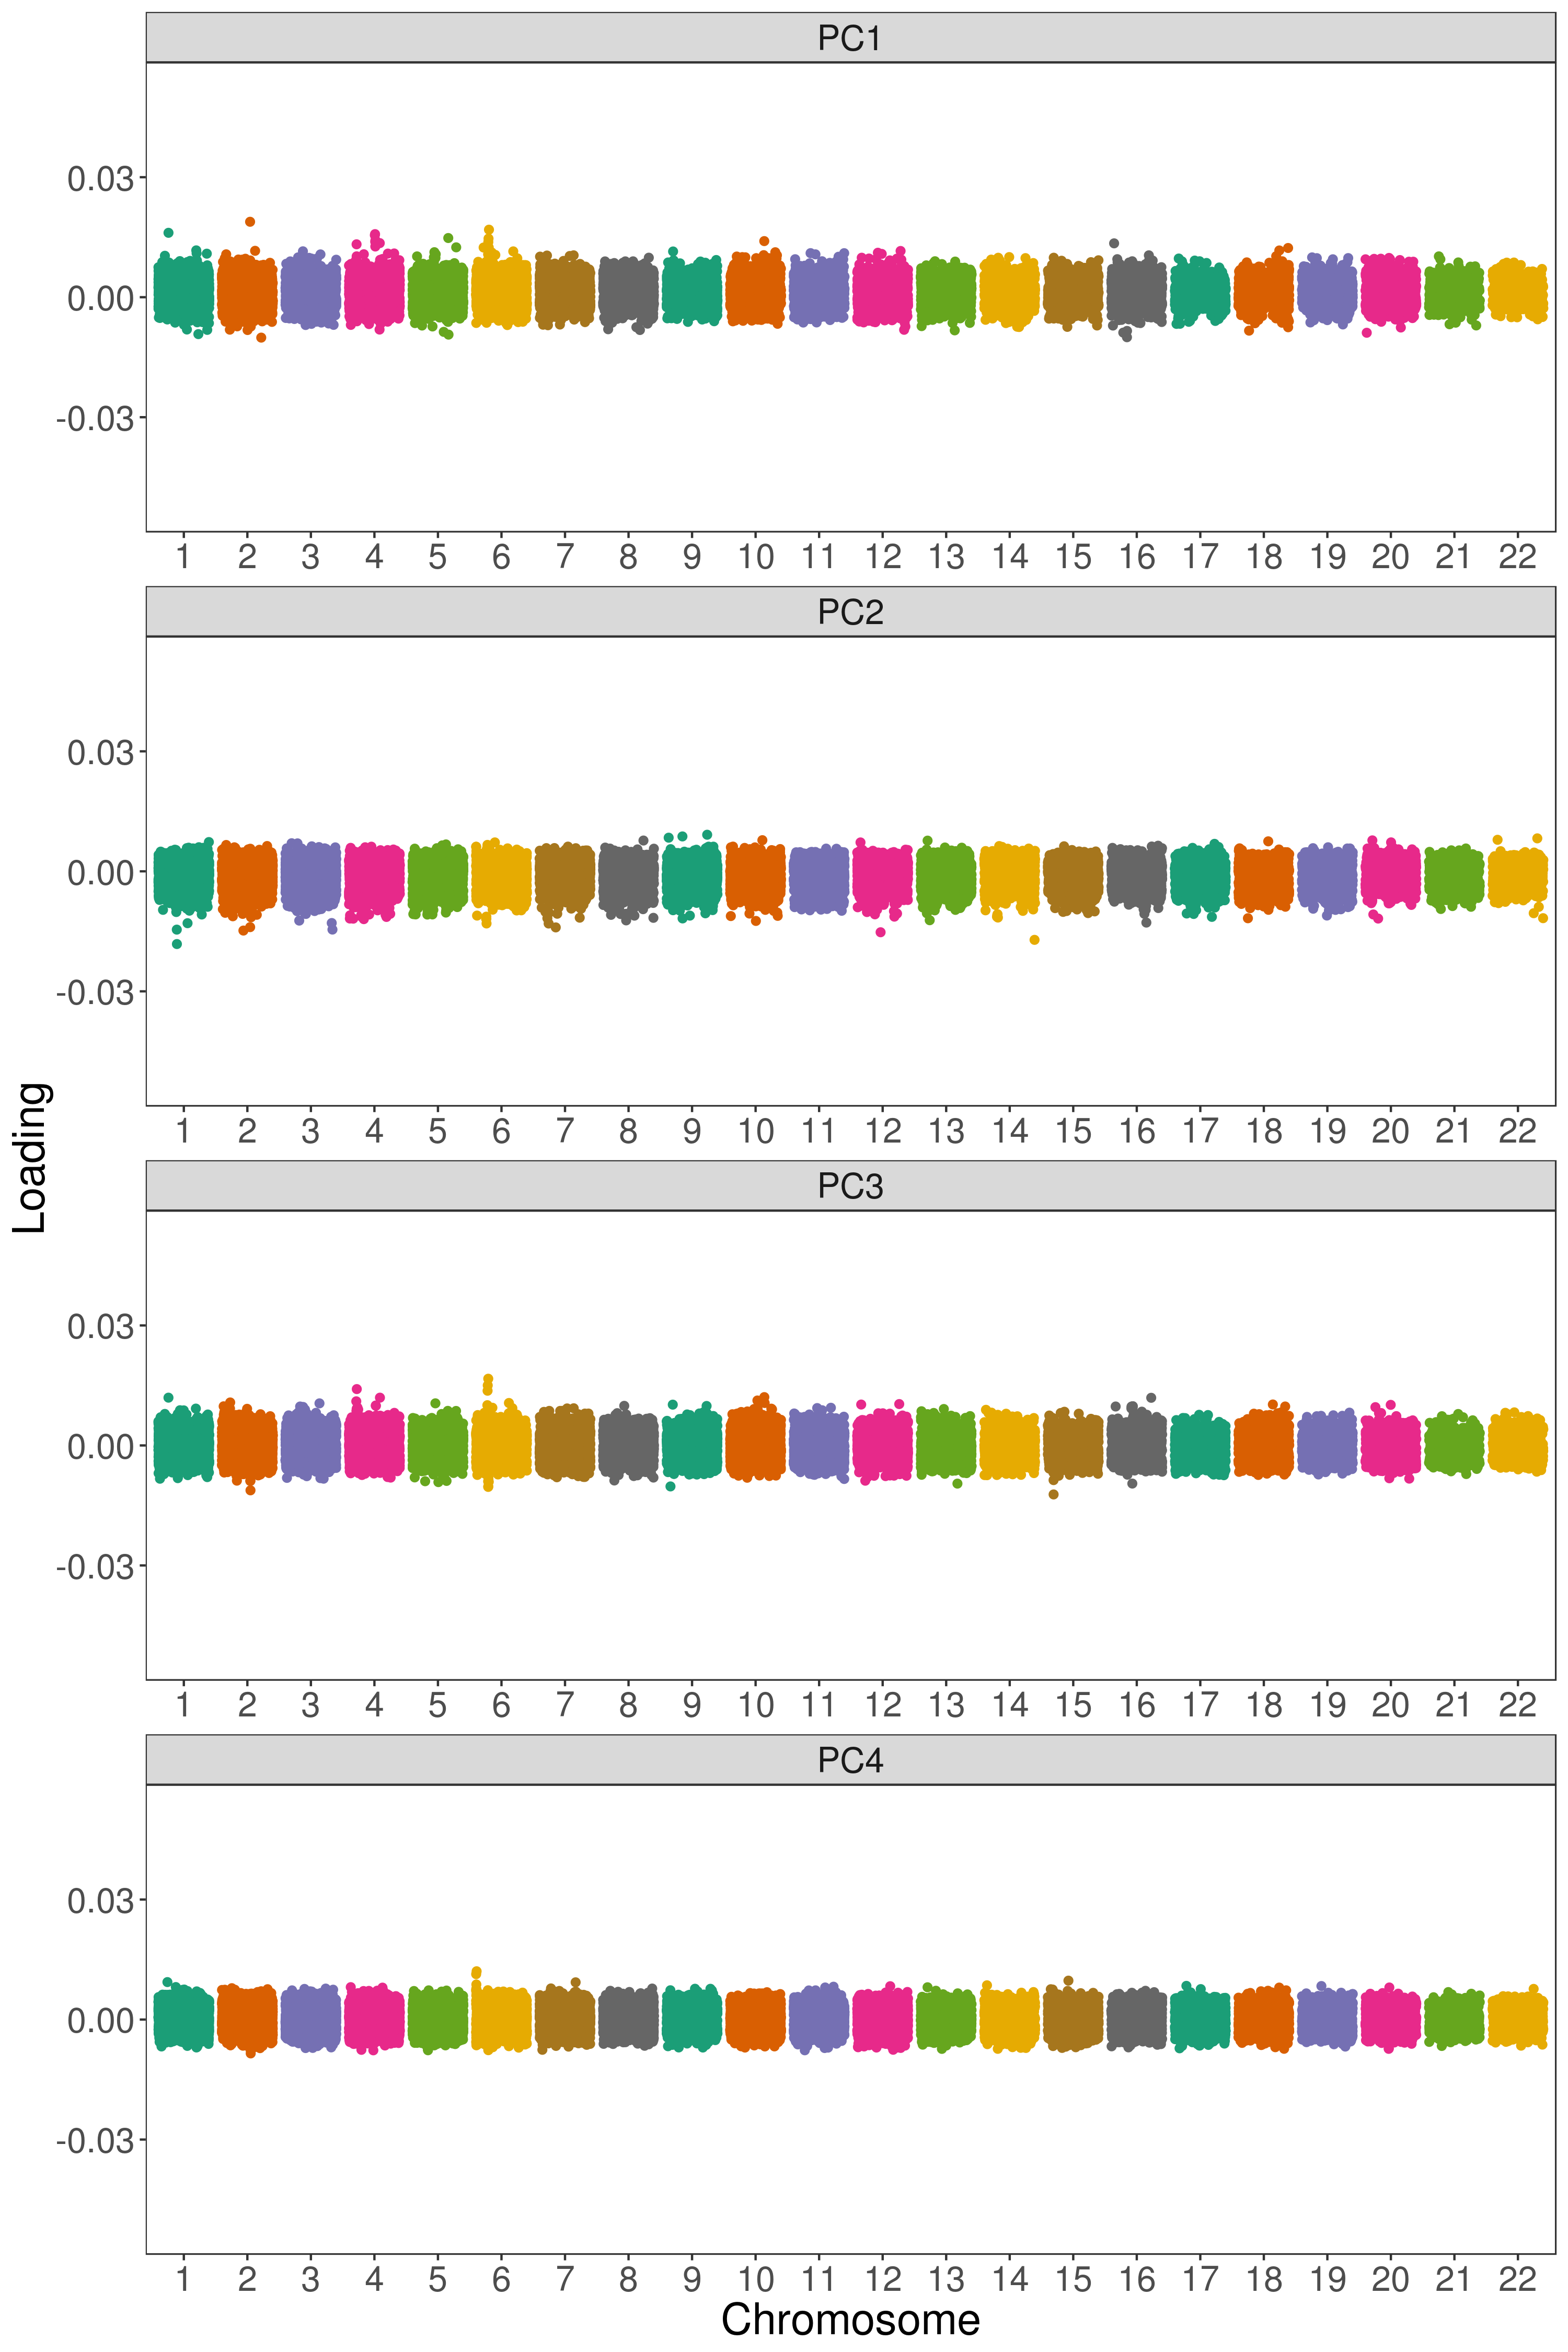
\includegraphics[width=0.32\paperwidth]{figs/EUR_prune_FALSE_0.2_0.5_0.01_snprelate_load_1}
%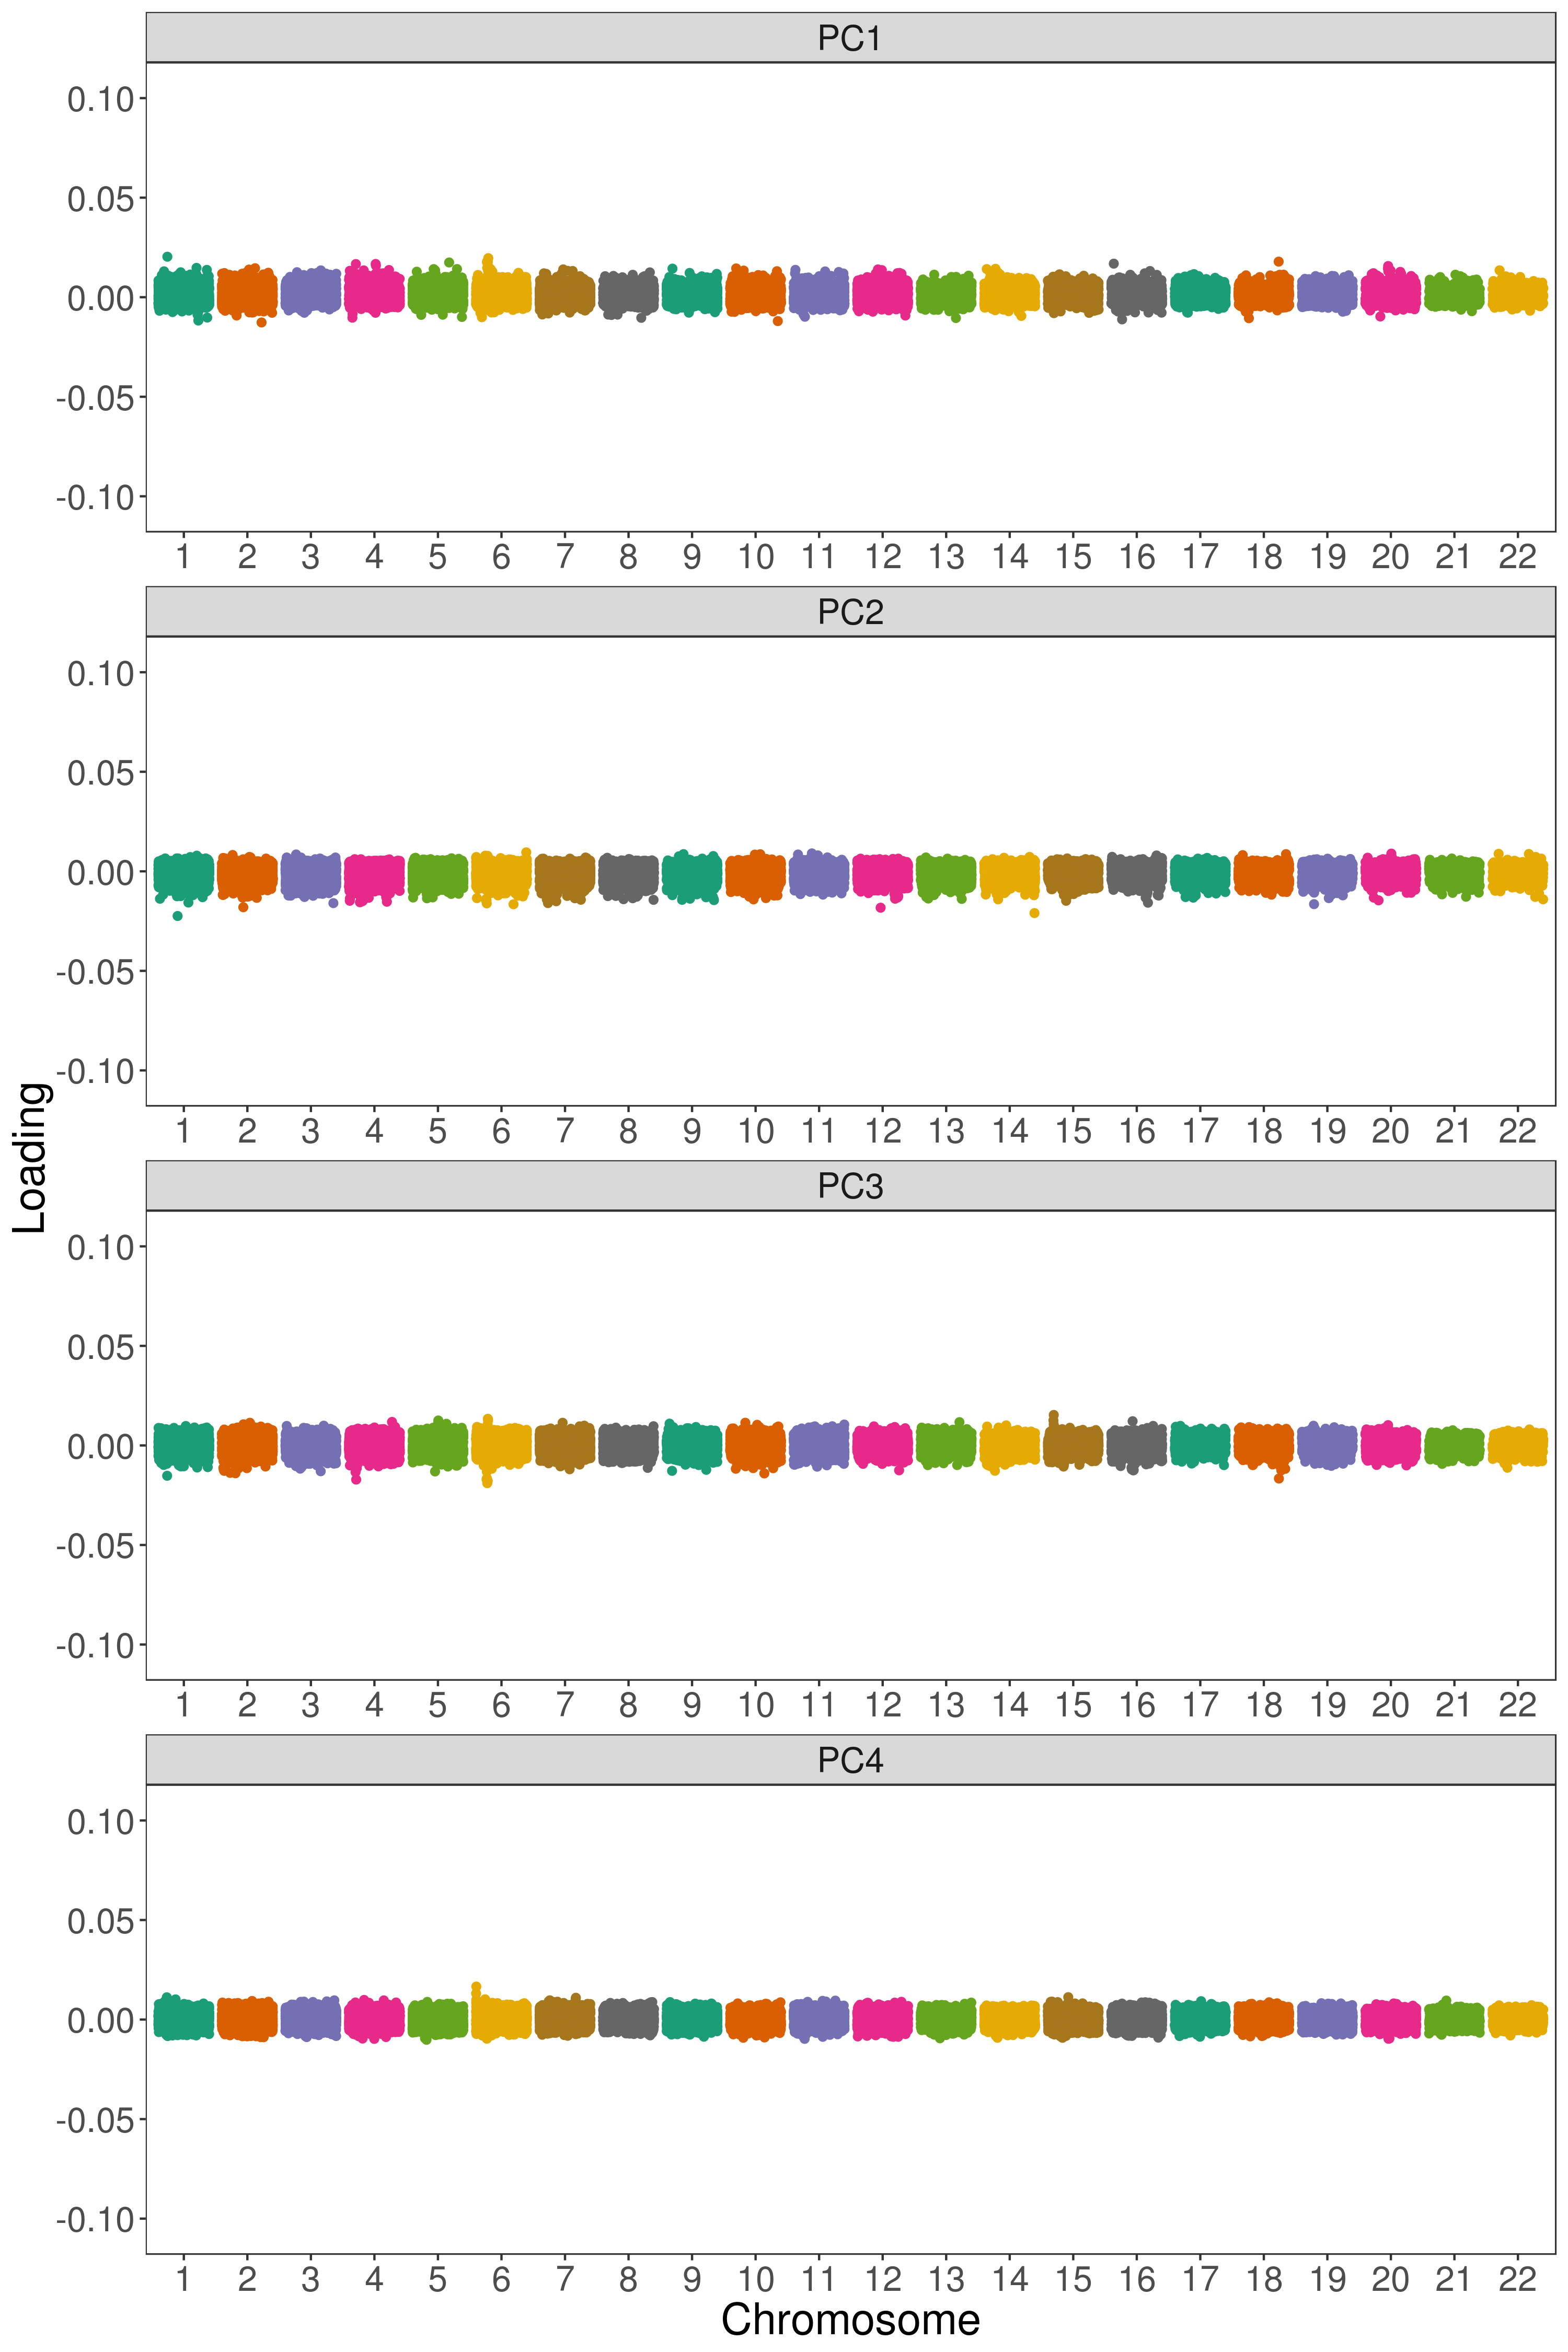
\includegraphics[width=0.32\paperwidth]{figs/EUR_prune_FALSE_0.1_0.5_0.01_snprelate_load_1}
%}
%\caption{SNP loadings for the first four principal components in COPDGene European Americans when previously-identified high-LD regions (Table \ref{tab:highLD}) are not removed prior to analysis but increasingly strict levels of LD pruning are performed. From left to right, columns correspond to no LD pruning, LD pruning with an $r^2$ threshold of 0.2 and a window size of 0.5 Mb, and LD pruning with an $r^2$ threshold of 0.1 and a window size of 0.5 Mb. \add{Change to look at correlation instead of loadings}}
%\end{figure}


%%% SKIP THIS -- write another paper on admixture mapping where this will be bigger focus
%\subsection{Confirming the importance of adjusting for population structure}
%
%\begin{itemize}
%\item show an example manhattan plot with no adjustment
%\item compare average number of spurious associations
%\item tie in theoretical results
%\end{itemize}


\subsection{Adjusting for PCs that capture local genomic features can induce spurious associations}

We have demonstrated that, especially without strict LD pruning, principal components can capture local genomic features rather than global ancestry in admixed populations.
However, it remains to be fully understood what the downstream implications would be of adjusting for these PCs in genome-wide association studies. 
We conducted a simulation study to investigate these implications further.

Figure \ref{fig:manh} presents Manhattan plots from one replicate of our simulation study.
In this setting, there is a single causal variant on chromosome 4, and we compare the results from genome-wide association studies in WHI SHARe African Americans using different ancestral heterogeneity adjustment approaches.
As expected, we see extreme inflation, i.e., statistically significant associations on \textit{every} chromosome, when we do not make any adjustment for ancestral heterogeneity (Panel A).
Otherwise, when we infer and adjust for ancestral heterogeneity using either PCA or a model-based approach, we see a single peak in our Manhattan plot on chromosome 4---as hoped, given that is where the causal variant is located---with one notable exception.
When we adjust for the first four principal components (as has been done in previous GWAS in WHI SHARe \citep{reiner2012, carty2012}), where those PCs were generated without any prior LD-based pruning or filtering, then we see a spurious association on chromosome 6 (Panel C).
However, this spurious association disappears if we only adjust for the first of these PCs (Panel B).
Likewise, no spurious association arises if we adjust for model-based admixture proportions (Panel D) or if we use PCs that were generated after LD pruning and Table \ref{tab:highLD} exclusions (Panels E and F).
Note that the causal variant, on chromosome 4, and the spurious signal, on chromosome 6, are both located in regions of the genome that are highly correlated with the PCs that were generated without any prior LD pruning (Figure \ref{fig:corr-compare}).

\begin{figure}[h]
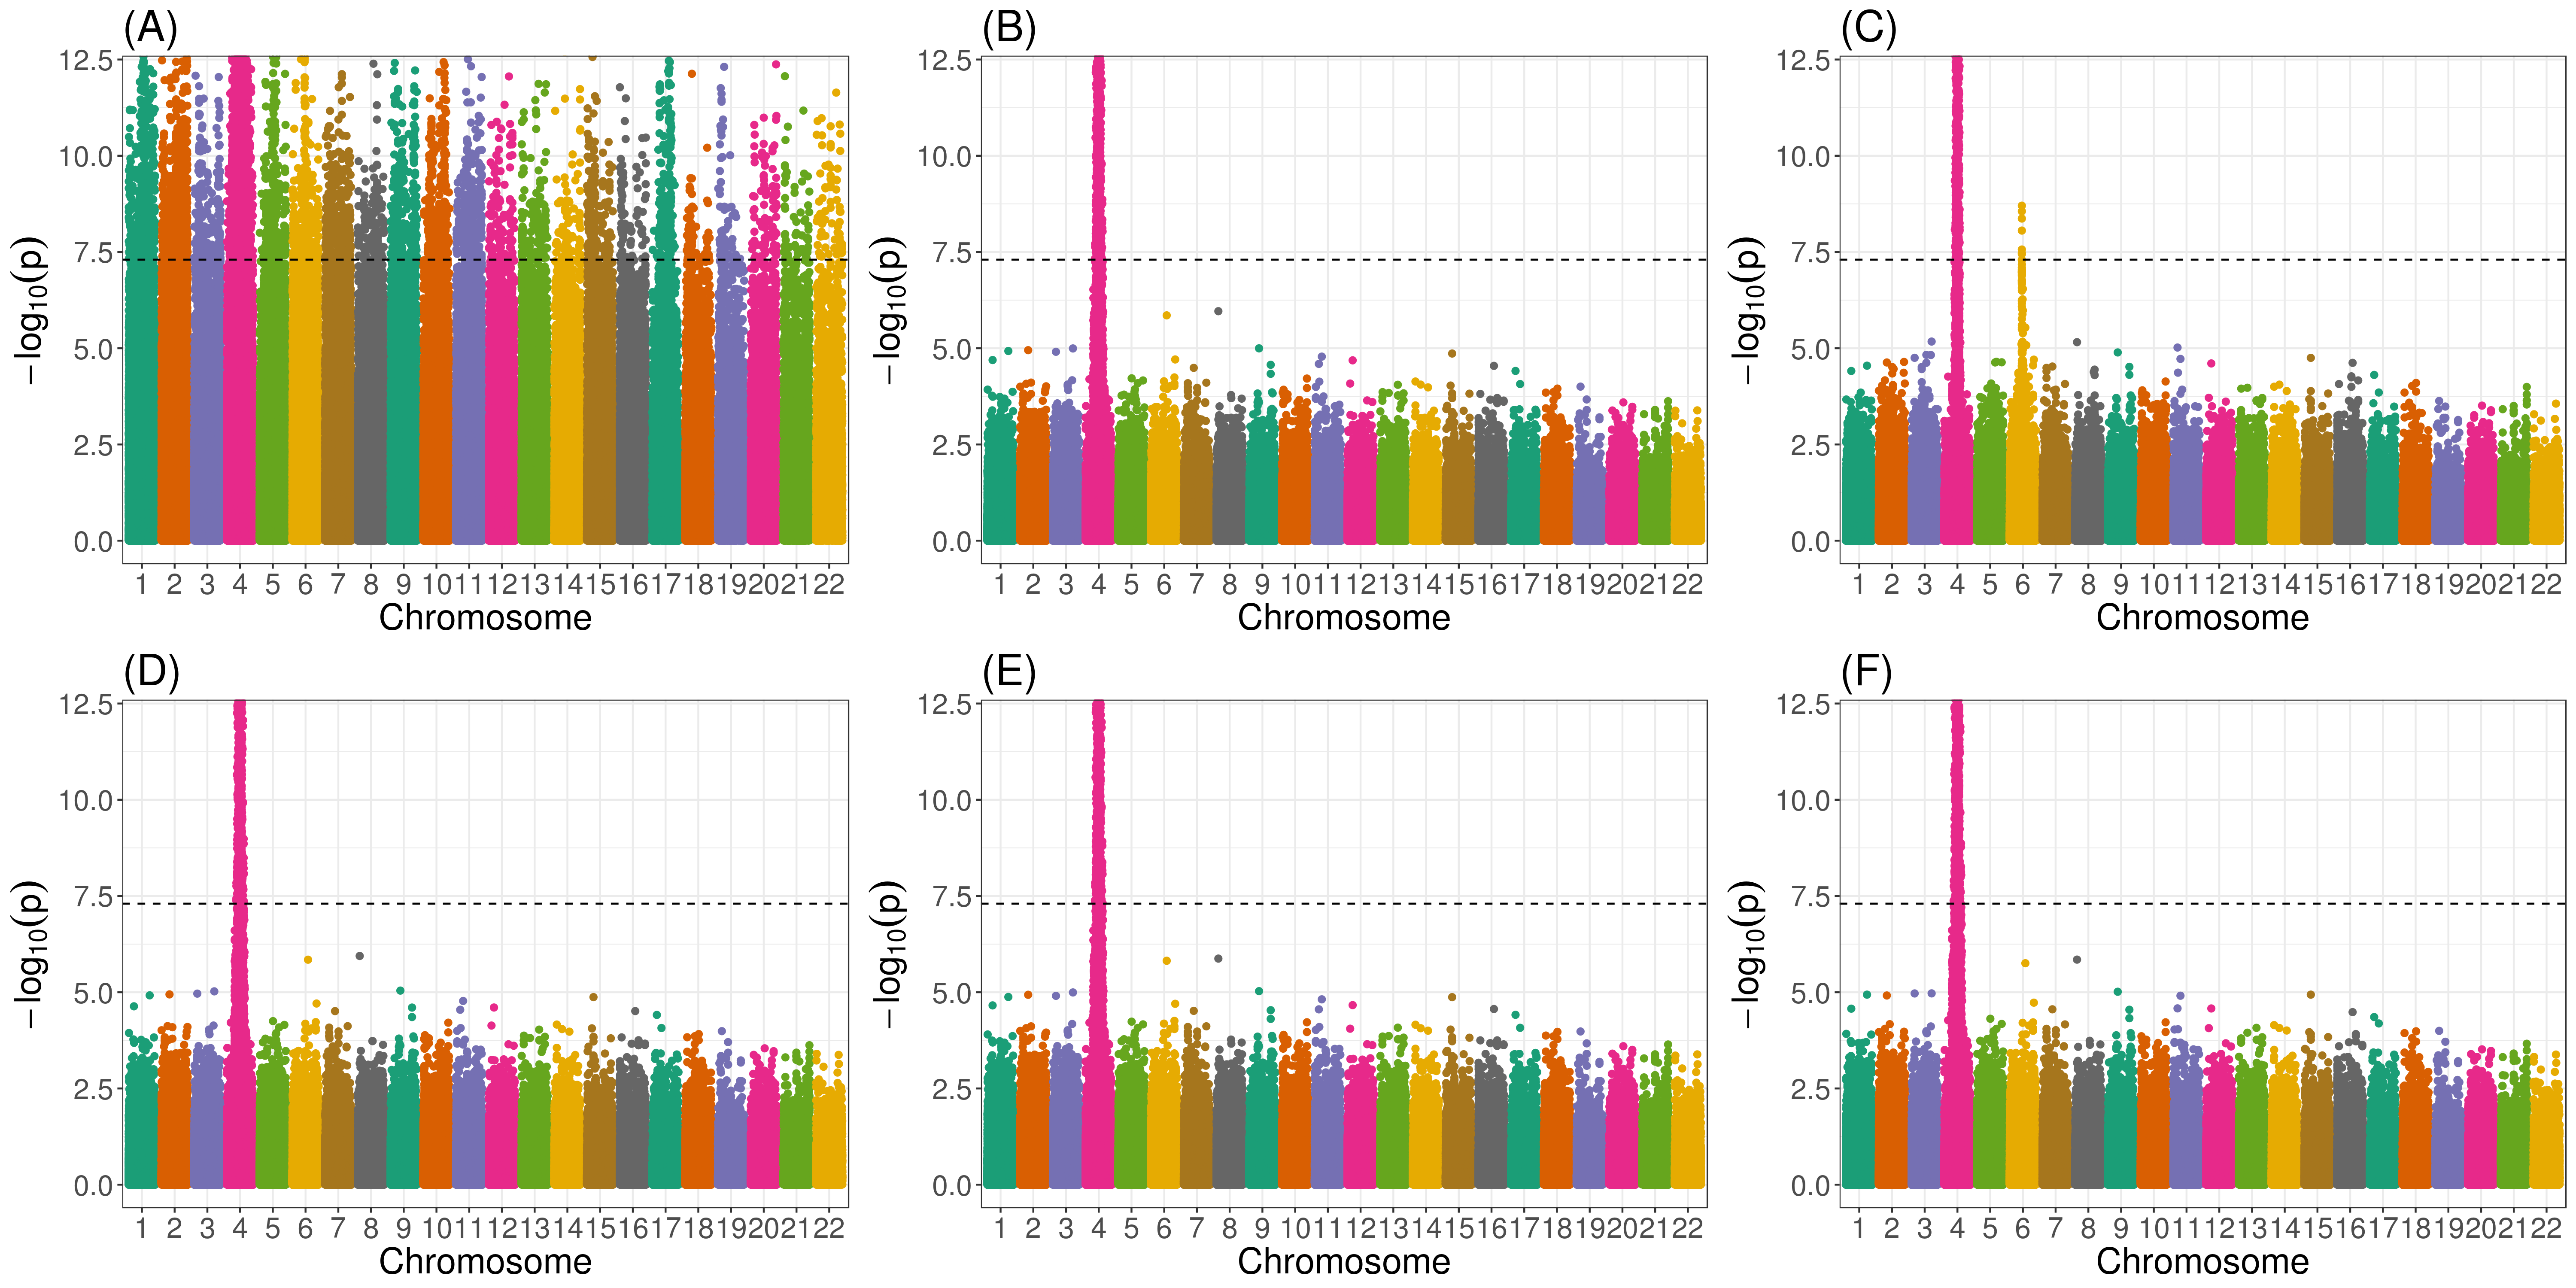
\includegraphics[width=\textwidth]{figs/manhattan/WHI_manh_gwas_70}
\caption{Manhattan plots from genome-wide association studies in WHI SHARe African Americans using different approaches to adjust for ancestral heterogeneity. In this example, the simulated trait depends only on the genotype at a single variant on chromosome 4: $y \sim N(g_{rs2036153}, 1)$. Panels present results using different adjustment approaches: (A) no adjustment; (B) one PC, with PCs calculated using all variants; (C) four PCs, with PCs calculated using all variants; (D) model-based admixture proportion estimates; (E) one PC, with PCs calculated after LD pruning ($r^2 < 0.1$, window size = 0.5 Mb) and Table \ref{tab:highLD} exclusions; and (F) four PCs, with PCs calculated after LD pruning and exclusions.}
\label{fig:manh}
\end{figure}

These results are not unique to this simulation setting. 
Figure \ref{fig:spurious} presents a comparison of the rate of spurious associations in genome-wide association studies in WHI SHARe African Americans.
We see that, across all simulation settings (Panel A), adjusting for PCs that capture local genomic features leads to higher numbers of spurious associations, on average.
Comparing models that make some sort of adjustment for ancestral heterogeneity, we observe the most spurious associations when GWAS models adjust for four principal components that were generated without any LD-based pruning or exclusions.
Excluding the high LD regions from Table \ref{tab:highLD} prior to running PCA reduces the number of observed spurious associations slightly, but not to the levels of the other approaches.
Given what we saw in Figure \ref{fig:corr-compare}, this is not surprising: even with these exclusions, PCs 2--4 still capture local genomic features---unless those exclusions are also combined with strict LD pruning.
We see fewer spurious associations when models adjust for model-based admixture proportions or principal components that do not capture local genomic features (i.e., using just the first PC, regardless of LD-based pruning or exclusions, or adjusting for four PCs when LD pruning was performed).
%Given the high correlation we observed between model-based admixture proportions  and PC1 (with or without LD-based pruning or exclusions), we see very similar results for these adjustment approaches.

\begin{figure}[h]
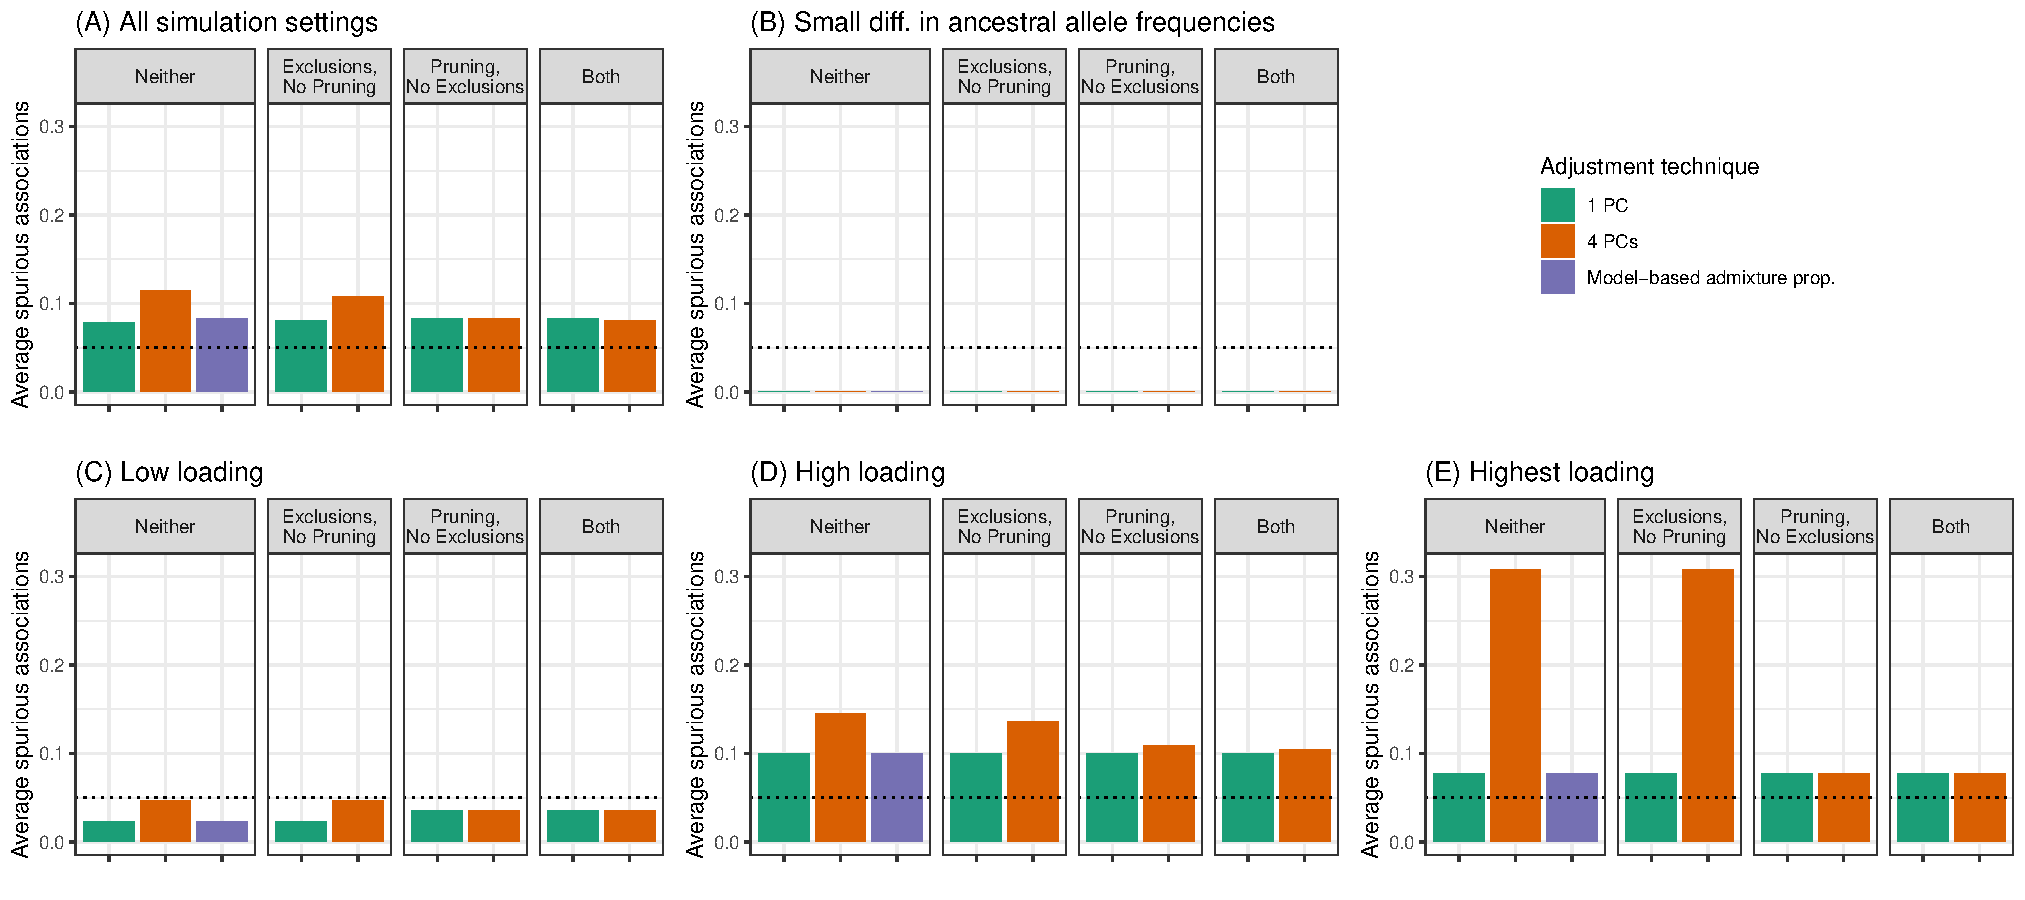
\includegraphics[width=\textwidth]{figs/spurious_counts/gwas/figure7_spurious_beta1}
\caption{Comparison of the number of spurious associations in genome-wide association studies in WHI SHARe African Americans using different approaches to adjust for ancestral heterogeneity. Panels display the average number of spurious associations that were observed across (A) all simulation settings, or across the subset of simulation settings in which the causal variant has (B) a small difference in ancestral allele frequencies, (C) low SNP loadings for each of the first four PCs, (D) a high SNP loading for at least one of the first four PCs, or (D) the highest SNP loading on its chromosome for one of the first four PCs. Within each panel, we compare the number of spurious associations when GWAS models adjust for model-based admixture proportions, 1 PC (with or without LD pruning and/or Table \ref{tab:highLD} exclusions), or 4 PCs (with or without LD pruning and/or Table \ref{tab:highLD} exclusions). Results shown here are for simulated traits with a single causal variant with an effect size ($\beta$) of 1. See Supplemental Figure \ref{fig:spurious-all-beta} for results with other choices of $\beta$.}
\label{fig:spurious}
\end{figure}


\subsection{Factors that influence the rate of spurious associations}

Our simulation results highlight various factors that influence when, and how many, spurious associations arise when adjusting for PCs that capture local genomic features.
% all approaches have no spurious assoc when there is small diff in allele freq at causal variant --- no confounding in this scenario, so really no need to adjust at all
First, we note that there are very few spurious associations, regardless of the adjustment approach (or even lack thereof), when there are small differences in ancestral allele frequencies at the causal variant (Figure \ref{fig:spurious}B). 
This is to be expected: in this scenario, the causal variant is not associated with global ancestry, so global ancestry is not a confounding variable (Figure \ref{fig:confounding}) and there is no need for adjustment.
% low for approaches that don't capture local genomic features
Considering other simulation settings in which the causal variant has a larger difference in ancestral allele frequencies (panels C, D, and E of Figure \ref{fig:spurious}), so adjusting for ancestral heterogeneity is needed, the number of observed spurious associations remains low for models that adjust for admixture proportions, a single principal component (regardless of pre-processing), or four PCs---if those PCs were were generated after strict LD pruning.
% correlation between PC and causal variant
For the two models that adjust for PCs capturing local genomic features (i.e., the models that adjust for 4 PCs that were generated with or without Table \ref{tab:highLD} exclusions, but no LD pruning), however, we see a higher rate of spurious associations, particularly when the causal variant is highly correlated with one of those PCs.
Notably, as the size of the causal variant's SNP loading increases from low (Figure \ref{fig:spurious}C), to high (Figure \ref{fig:spurious}D), to the highest on its chromosome (Figure \ref{fig:spurious}E), we see an increasing number of spurious associations for these two approaches.
This confirms the pattern we saw in Figure \ref{fig:manh}, where a spurious association arose when we adjusted for PCs that were highly correlated with variants in several regions across the genome, and both the causal variant and spurious signal were located in one of those regions. 
% effect size of causal variant
Finally, we note that these problems worsen as the effect size of the causal variant increases (see Supplemental Figure \ref{fig:spurious-all-beta}).

To better understand the patterns observed in our simulation study, we compare the expected effect size estimates from GWAS models in admixed populations with two ancestral populations using different techniques for adjusting for ancestral heterogeneity.
As in our simulations, we assume that the trait depends on a single causal variant: $$y_i \stackrel{iid}{\sim} N(\beta_1 g_{i1} + \beta_\pi \pi_i, 1),$$ where $g_{i1}$ represents the number of minor alleles carried by individual $i$ at the causal variant, which we will refer to as \textit{Variant 1}, and $\pi_i$ is the individual's admixture proportion.
(Note that $\beta_\pi = 0$ in our simulation study, but we consider the more general setting here.)
We can then derive the expected effect size estimate at that causal variant, as well as a second variant that is not associated with the trait and sits on a different chromosome than the causal variant.
When we consider a GWAS model that adjusts for the true admixture proportions,
%$\pi_i$, $$E[y_i | g_{ij}, \pi_i] = \beta_0 + \beta_j g_{ij} + \beta_\pi \pi_i,$$ 
the expected effect size estimates at the causal variant (Variant 1) and the unlinked neutral variant (Variant 2) are
$$
\begin{aligned}
E[\hat\beta_1] &= \beta_1 \\
E[\hat\beta_2] &= 0,
\end{aligned}
$$
where $\beta_1$ is the true effect size of the causal variant and $\beta_2 = 0$ is the true effect size of the neutral variant.
In other words, models that perfectly adjust for ancestral heterogeneity will yield unbiased estimates of the effect size at the causal and unlinked neutral variants.
%This suggests, in turn, that these models will control the rate of spurious associations.

% unadjusted model
In comparison, GWAS models that do not make any adjustment for ancestral heterogeneity will yield effect size estimates of
$$
\begin{aligned}
E[\hat\beta_1] & = \beta_1 + \frac{(p_{11}- p_{10})V_\pi \beta_\pi }{p_{10}(1-p_{10}) + (p_{11}-p_{10})(1-p_{11}-p_{10})E_\pi + (p_{11}-p_{10})^2(V_\pi + E_\pi - E_\pi^2)} \\
E[\hat\beta_2] & = 0 + \frac{(p_{21}-p_{20}) V_\pi\{\beta_\pi + 2\beta_1(p_{11}- p_{10})\}}{p_{20}(1-p_{20}) + (p_{21}-p_{20})(1-p_{21}-p_{20})E_\pi + (p_{21}-p_{20})^2(V_\pi + E_\pi - E_\pi^2)},\\
\end{aligned}
$$
where $E_\pi, V_\pi$ are the population mean and variance of the admixture proportions, $\beta_\pi$ is the direct effect of admixture proportions on the trait, $p_{11}, p_{10}$ are the allele frequencies of the causal variant in the two ancestral populations, and $p_{21}, p_{20}$ are the ancestral allele frequencies of the unlinked neutral variant.
From these results, we see that the unadjusted model will yield a biased estimate of the effect size of the causal variant ($E[\hat\beta_1] \neq \beta_1]$) unless there is no ancestral heterogeneity (i.e., $V_\pi = 0$), global ancestry does not have a direct effect on the trait (i.e., $\beta_\pi = 0$), or the causal variant does not have different allele frequencies in the ancestral populations (i.e., $p_{11} = p_{10}$). 
We see, also, that the model can yield a biased effect size at the unlinked neutral variant ($E[\hat\beta_2] \neq 0$) even if global ancestry does not have a direct effect on the trait, provided that both the causal variant and the variant being tested have allele frequencies that differ between the two ancestral populations (i.e., $p_{11} \neq p_{10}$ and $p_{21} \neq p_{20}$).
These biased effect size estimates at neutral variants will translate into spurious associations as sample sizes increase, just as we saw in our simulations (Figure \ref{fig:manh}A and Supplemental Figure \ref{fig:spurious-all-beta}).
These results are summarized in Figure \ref{fig:confoundingdags} and underscore the importance of adjusting for ancestral heterogeneity even when global ancestry does not have a direct effect on the trait.

\begin{figure}
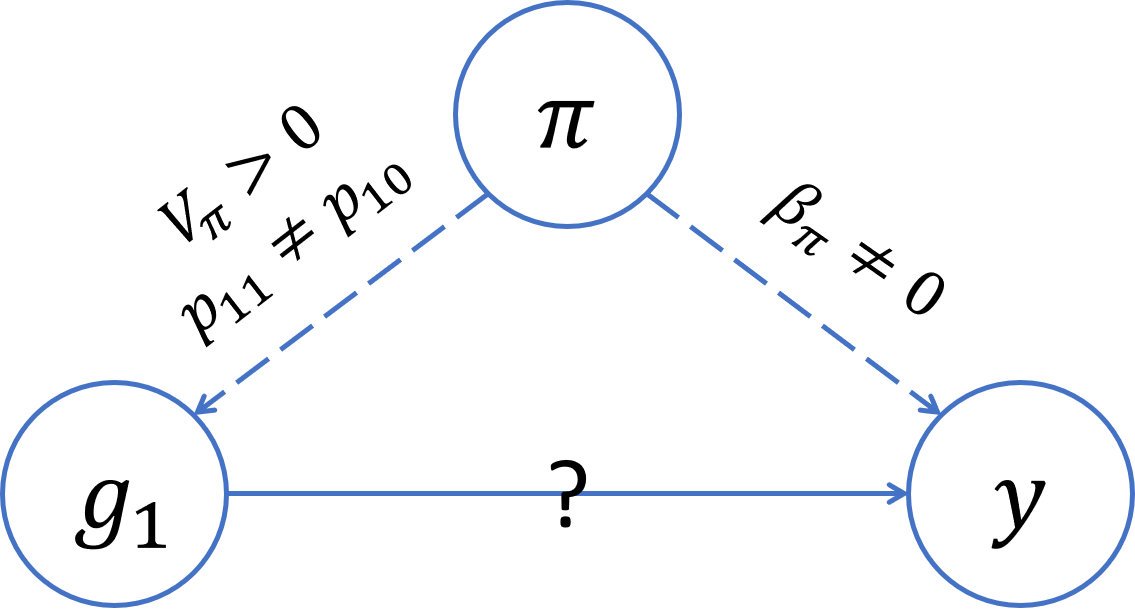
\includegraphics[width=0.45\textwidth]{figs/confounding_dags/dag_gwas_1_v2.png}
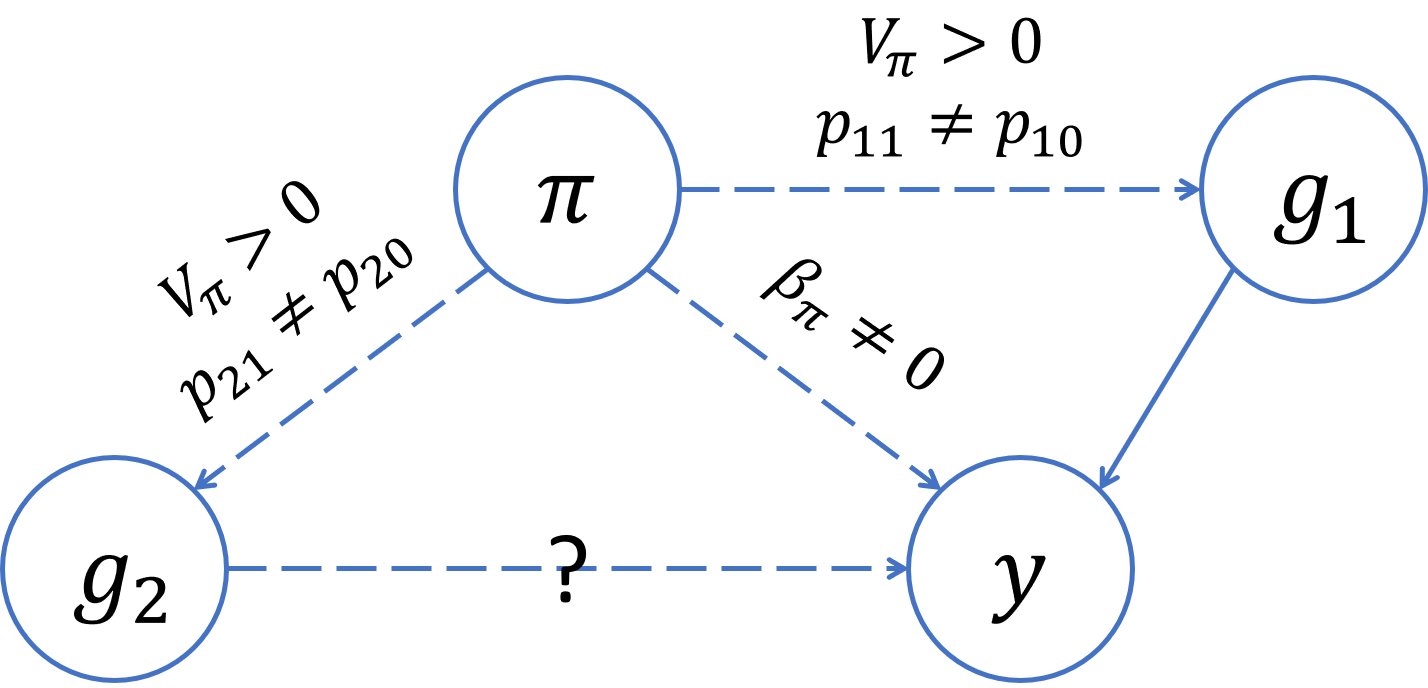
\includegraphics[width=0.55\textwidth]{figs/confounding_dags/dag_gwas_2_v2.png}
\caption{Conditions for confounding by global ancestry in GWAS. \\(A) Global ancestry confounds the association at the causal variant (Variant 1) if there is ancestral heterogeneity in the population ($V_\pi > 0$), the causal variant has different allele frequencies in the ancestral populations ($p_{11} \neq p_{10}$), and global ancestry has a direct effect on the trait ($\beta_\pi \neq 0$). \\(B) Global ancestry can confound the association at an unlinked neutral variant (Variant 2) even if global ancestry does not have a direct effect on the trait ($\beta_\pi = 0$), provided that there is ancestral heterogeneity ($V_\pi > 0$) and both the causal variant and the variant being tested have different allele frequencies in the ancestral population ($p_{11} \neq p_{10}, p_{21} \neq p_{20}$).}
\label{fig:confoundingdags}
\end{figure}


% results with two PCs
To emulate the idea of adjusting for principal components that adjust for local genomic features, we also consider a scenario in which our GWAS model adjusts for two ``principal components".
We assume that the first principal component captures global ancestry (i.e., $\mathbf{u}_1 = \boldsymbol\pi$) but the second principal component captures some feature other than global ancestry (i.e., $\mathbf{u}_2 = \mathbf{z}$ for some variable $z$).
Then, we can show that the expected effect size estimates at the causal variant and an unlinked neutral variant will be
$$
\begin{aligned}
E[\hat\beta_1] & = \beta_1 \\
E[\hat\beta_2] & = 0 + \beta_1 \frac{-V_\pi E\{\text{Cov}(g_1, z \mid \pi)\} E\{\text{Cov}(g_2, z \mid \pi)\}}{V_z(V_\pi V_{g_2} - C_{g_2,\pi}^2) - V_\pi C_{g_2,z}^2 + C_{\pi, z}(2C_{g_2,\pi} C_{g_2,z} - V_{g_2}C_{\pi,z})}, \\
\end{aligned}
$$
where $V_a = \text{Var}(a)$ and $C_{a,b} = \text{Cov}(a,b)$.
We see that this model adjusting for an extraneous principal component will yield an unbiased effect size estimate at the causal variant, but the same is not true for the unlinked neutral variant.
In particular, the effect size estimate at this neutral variant will be biased away from zero when there is  ancestral heterogeneity (i.e., $V_\pi \neq 0$) and the second principal component is correlated with both the causal variant and the variant being tested (i.e., $\text{Cov}(g_1, z \mid \pi) \neq 0$ and $\text{Cov}(g_2, z \mid \pi) \neq 0$).
In other words, these results indicate that a model that adjusts for a PC that captures genotype at the causal variant as well as a second variant that is not associated with the trait, then spurious associations will arise at that second neutral variant in large enough samples.
This is exactly what we observe in our simulations (Figure \ref{fig:manh}C, Figure \ref{fig:spurious}D,  Figure \ref{fig:spurious}E).
However, if the extra PC does not capture genotype at the causal variant, then spurious associations will not arise (Figure \ref{fig:manh}F, Figure \ref{fig:spurious}C).

% 
Proofs and simulations validating these analytic results are available in the Appendix.

% connect to idea of collider bias
%\add{connect to collider bias --- or save for discussion?}

%% skip for now unless requested by co-author or reviewer
%how does FWER compare?
%\begin{itemize}
%\item manhattan plots for one or two simulated traits
%\item overall summary of rejection rates
%\item is it appropriate to use same significance threshold for all?
%\end{itemize}
% do they have similar power?  --- this is easier to do b/c can use existing simulations


\section{Discussion}

% explain significance of results and place them in broader context
% may contain subheadings

%\edit{(See dissertation: \href{https://digital.lib.washington.edu/researchworks/handle/1773/44730}{https://digital.lib.washington.edu/researchworks/handle/1773/44730})}

% summary of major takeaways
\edit{Our work above reiterates the importance of adjusting for ancestral heterogeneity in genome-wide association studies in admixed populations and the need for careful consideration of the techniques used to make such an adjustment.
Through theoretical work, simulation studies, and analysis of three admixed populations (WHI SHARe, TOPMed JHS, and TOPMed COPDGene African Americans) ...
Highlights X important takeaways.}
%Of particular note, we have shown that approaches based on principal component analysis (PCA) can actually \textit{induce} spurious associations unless careful pre-processing is conducted prior to running PCA. 
%These results are particularly concerning given the wide-spread use of PCA to control for ancestral heterogeneity in GWAS.

%\noindent Need to address ancestral heterogeneity in admixed populations
We see considerable variability in global ancestry proportions across WHI SHARe, TOPMed JHS, and TOPMed COPDGene African Americans (Figure \ref{fig:barplots}), as is true in many other admixed populations.
It is widely understood that adjusting for this ancestral heterogeneity is important for GWAS, given that global ancestry is a potential confounding variable (Figure \ref{fig:confounding}). %but the conditions under which this confounding may arise are not fully understood.
Our simulations and theoretical work confirm that global ancestry can confound the association between a genetic variant and the trait --- thus opening the door to spurious associations --- even when it does not have a direct effect on the trait itself, provided that there is a causal variant elsewhere in the genome that has different allele frequencies across the ancestral populations of interest (Figure \ref{fig:confoundingdags}).
Although this fact has been recognized previously \add{CITE 143}, it seems to have been forgotten by some.
Our theoretical work explicitly demonstrates the factors that impact the magnitude of the bias incurred by GWAS models that fail to adjust for global ancestry, and the conditions under which that bias may arise.
We hope that our results will serve as a reminder to researchers of the various ways in which global ancestry can confound genetic studies in admixed populations and the importance of ensuring that GWAS models appropriately adjust for ancestral heterogeneity.
%\begin{itemize}
%\item we observe considerable heterogeneity in global ancestry proportions in admixed populations studied here, as in other studies 
%\item well-established that global ancestry is a potential confounding variable
%\item this confounding can exist even if global ancestry does not have a direct effect on the trait (as demonstrated by our simulation studies and theoretical results)
%\item $\rightarrow$ important to carefully measure and adjust for ancestral heterogeneity in GWAS in admixed populations
%\end{itemize}

%\noindent Comparing (naive) PCs and admixture proportions
Two common approaches for adjusting for ancestral heterogeneity in GWAS involve including global ancestry as a covariate in marginal regression models, with global ancestry estimated using either model-based approaches or principal component analysis.
In WHI SHARe, TOPMed JHS, and TOPMed COPDGene African Americans, the first principal component is highly correlated with model-based estimates of the genome-wide proportion of African ancestry (Figure \ref{fig:pcsvsglob}) and models adjusting for either perform similarly.
Later PCs, however, do not correlate with global ancestry and seem instead to capture local genomic features, particularly when PCs are generated without any prior LD pruning (Figures \ref{fig:corr-TOPMed} and \ref{fig:corr-compare}).
A similar phenomenon has been documented before \add{CITE: Zou, Prive, Price?}, with authors observing that PCs can pick up regions with high, extensive, or otherwise unusual patterns of linkage disequilibrium (e.g., \textit{HLA}, inversions).
%The phenomenon presents somewhat differently in admixed populations, however, which is perhaps not unsurprising given that LD patterns are known to differ between admixed populations and populations with European ancestry.
However, in contrast to what was observed in those studies---all of which involved individuals of European ancestry---we see in our admixed samples that a single PC often captures variants on \textit{multiple} chromosomes (i.e., there are multiple peaks in the SNP loading plots, rather than just a single peak).
This has important downstream implications.
%\begin{itemize}
%\item both widely used for measuring and adjusting for ancestral heterogeneity
%\item in AA, first PC correlated with global ancestry but later PCs are not (in HL: TBD)
%\item instead, later PCs often capture local genomic features (e.g., regions with extensive LD)
%\item while this has been documented before, note that, in contrast to what has been observed in EUR, we see that PCs seem to capture SNPs on more than one chromosome (multiple peaks in SNP loading plots); whereas in EUR we often just see one peak (cite Zou, Prive, other examples?) $\rightarrow$ why? LD patterns in admixed pops differ from those in EUR %% in discussion, note how this differs from what had previously been seen in Europeans (one peak vs multiple peaks, weaker pruning); refer to COPD example in supplement
%\end{itemize}

%\noindent Spurious associations
Our simulations and theoretical work show that models that adjust for PCs capturing multiple local genomic features have elevated rates of spurious associations, with the number of spurious associations increasing with the effect size of the causal variant and the strength of the correlation between that causal variant and the PC by which it is captured.
This can be explained by the concept of \textit{collider bias} (Figure \ref{fig:collider}).
Suppose that, instead of capturing genome-wide global ancestry, a PC is driven instead by the genotype of two variants on distinct chromosomes ($g_1, g_2$). 
If one of those variants ($g_1$) is associated with the trait, then the PC becomes a \textit{collider variable}, rather than a confounding variable, when testing the association between the other variant ($g_2$) and the trait.
Adjusting for the PC can then induce a spurious association between the trait and the neutral variant as a result of collider bias \add{CITE 71}.
Prior work has shown that adjusting for heritable covariates (e.g., height, body mass ndex) can induce collider bias in GWAS \add{CITE 144, 145}, and that principal components can induce collider bias in gene expression studies \add{CITE 146}, but the issues posed by PCs to GWAS have not been previously demonstrated.
\edit{\begin{itemize}
%\item adjusting for these PCs can lead to spurious associations
%\item this is due to a phenomenon known as collider bias
\item ADD: what do theory and sims tell us about when/how likely a spurious association is to occur? (what's \textit{realistic}? -- refer to gene expression paper)
\item ADD: could spurious associations replicate? (given that peaks often occur in similar places across datasets)
%\item prior work on collider bias in GWAS
\end{itemize}}

\begin{figure}
\begin{center}
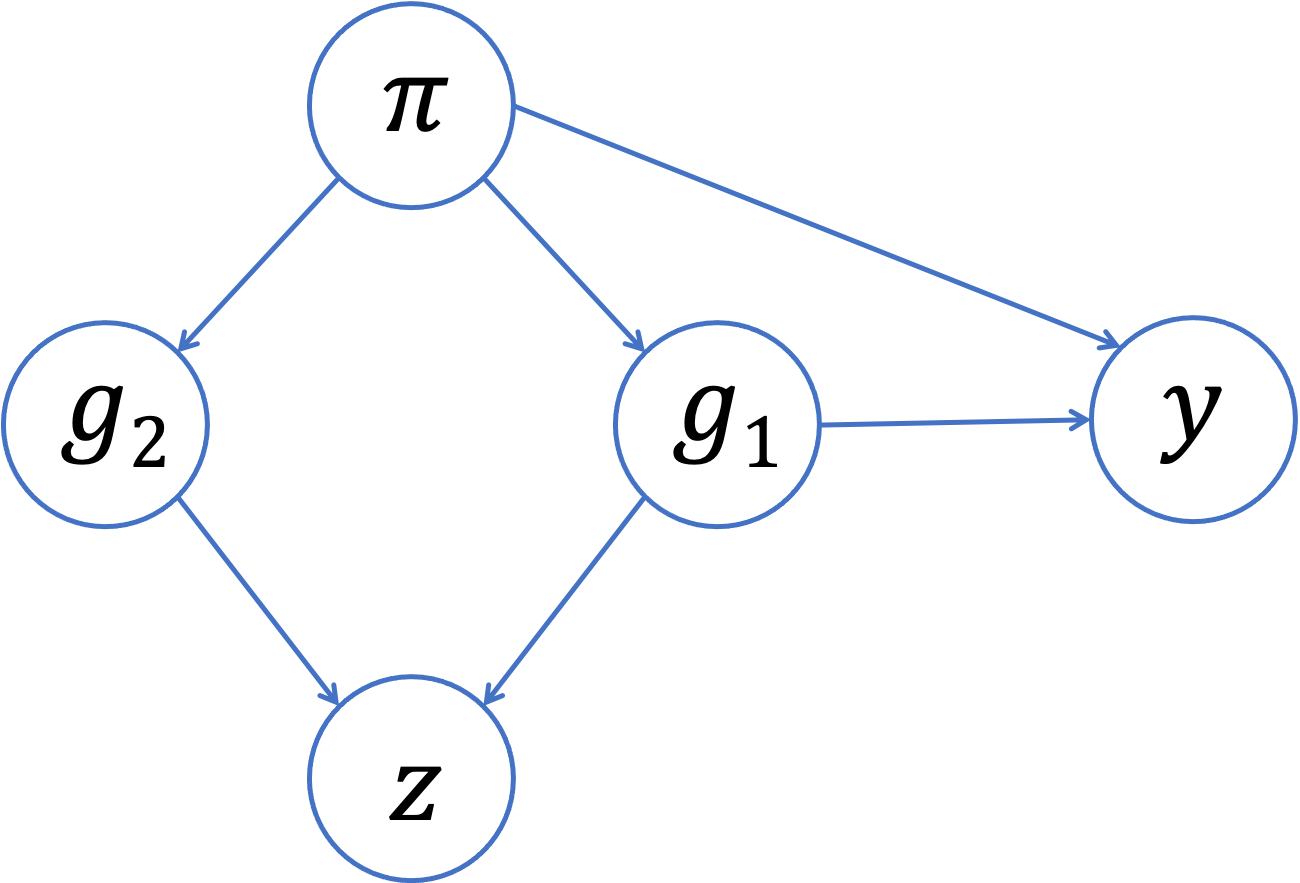
\includegraphics[width=0.5\textwidth]{figs/confounding_dags/dag_collider.png}
\caption{Collider bias in GWAS.\add{ADD MORE}}
\end{center}
\label{fig:collider}
\end{figure}

%\noindent Impact of LD pruning and removing high LD regions
In our analysis of genotype and sequence data from unrelated WHI SHARe, TOPMed JHS, and TOPMed COPDGene African Americans, we found that all but the first principal component were largely driven by small regions of the genome---and thus have the potential to be collider variables---unless careful pre-processing of genotype data was preformed prior to running PCA.
As mentioned earlier, previous studies have found that PCs can capture small regions of the genome, and as a result have suggested that these regions be excluded (Table \ref{tab:highLD}) and/or that LD pruning be performed prior to running PCA \add{CITE}.
However, the motivation for this LD-based filtering has typically been framed in terms of the ability of the principal components to capture global ancestry, as well as the computational complexity of running PCA, rather than the downstream implications on association testing that we have highlighted here.
Furthermore, we have found that excluding the regions listed in Table \ref{tab:highLD} does not resolve these issues in admixed populations: in WHI SHARe, for example, we still see peaks in the PC-genotype correlation plots (Figure \ref{fig:corr-compare}) and models adjusting for this set of PCs still show elevated rates of spurious associations (Figure \ref{fig:spurious}).
We have also found that identifying  and removing potentially problematic regions based on our own data is tedious and does not provide any benefit beyond LD pruning \add{CITE appendix}, and that a stricter threshold ($r^2$ = 0.1) is needed for LD pruning than is often suggesed in the literature \add{CITE appendix}.
The vast majority of previous recommendations were based on studies in European populations, but LD patterns can be very different in admixed populations. 
In particular, LD typically extends much further (even across chromosomes) \add{CITE 147, 148}, so it makes sense that stricter levels of LD-based filtering would be required.
\edit{\begin{itemize}
%\item after LD pruning, PCs no longer exhibit patterns of being driven by select few SNPs (at least for PCs 2-4)
%\item note that we had to use smaller $r^2$ than often recommended in literature for this to be true (refer to supplemental figure) $\rightarrow$ why? LD patterns in admixed pops differ from those in EUR 
%\item excluding previously-identified high LD regions doesn't seem to be as effective $\rightarrow$ why? LD patterns in admixed pops differ from those in EUR
%\item mention data-based exclusions approach (add supplemental figure)
\item note, too, that even strict LD pruning doesn't seem to remove all correlation between SNPs and genotypes (e.g., later PCs in WHI, TOPMed COPDGene)
\end{itemize}}

\noindent Limitations/practical implications

\noindent Recommendations
\begin{itemize}
\item If using PCs, carefully inspect SNP loadings and/or correlation between PCs and genotypes
\item If using PCs, don't use more than you need
\item Consider using global ancestry proportions (although further work is needed to reliably capture sub-continental structure)
\end{itemize}

%a possible paper to cite: https://www.biorxiv.org/content/10.1101/2022.03.25.485885v1.full
%%says "Our tests also found PCA robust to large numbers of PCs, far beyond the optimal choice, agreeing with previous anecdotal observations (Price et al., 2006 "PCA corrects for strafication..."; Kang et al., 2010 "Variance component model to account...") in contrast to using too few PCs for which there is a large performance penalty."


% future work: 
%% GWAS vs admixture mapping
%% sequence vs genotype data
%% how does this apply to mixed models?


\newpage
\section{Appendix}

% can put detailed results of statistical analyses here
% may contain subheadings

\begin{itemize}
\item theoretical results
\item proofs
\item simulations validating theory
\end{itemize}


\newpage
\section*{Supplemental Data}

% briefly list what types of data are included in supplemental data (a separate PDF document)
% e.g., "Supplemental Data include four figures and two tables"

Supplemental Data include \add{??} figures and \add{??} tables.

\begin{figure}[h]
\center
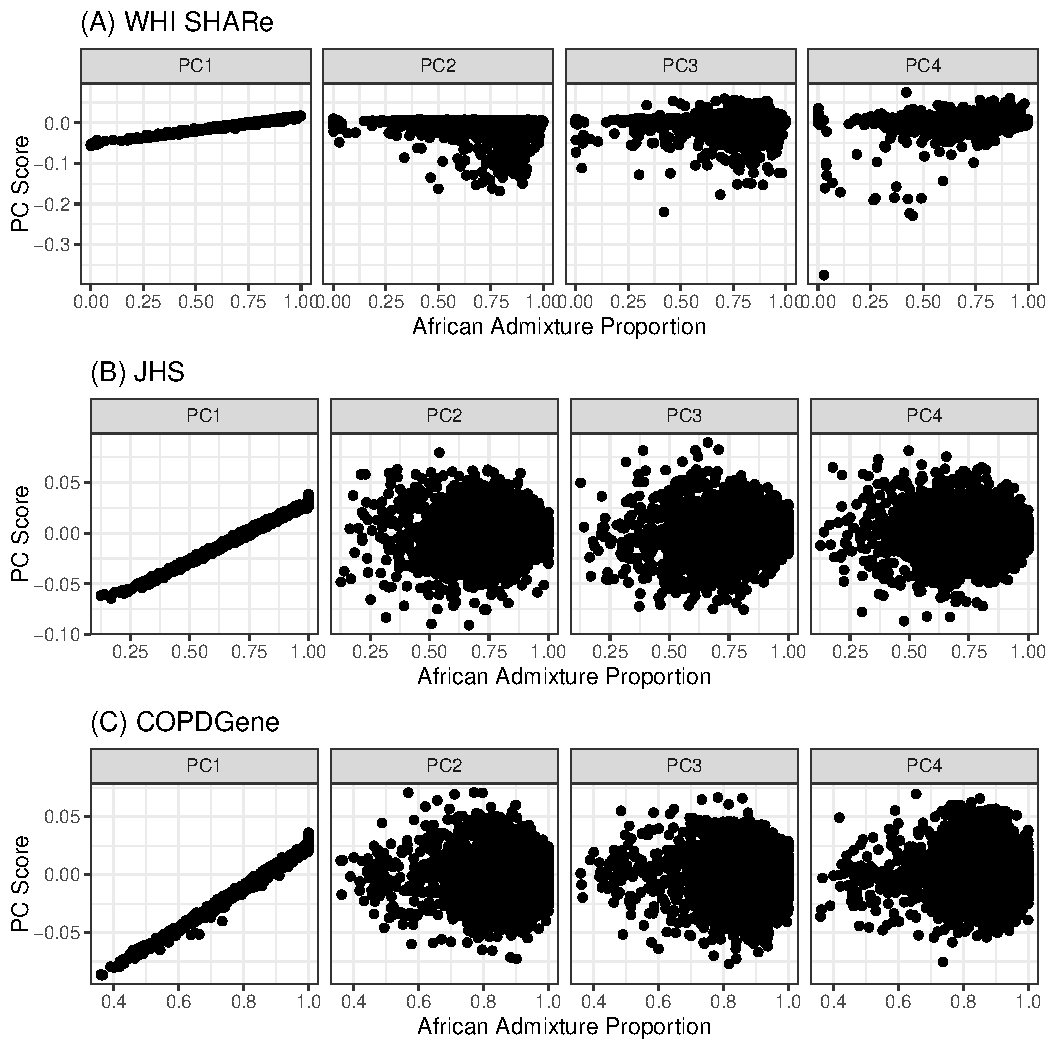
\includegraphics[width=\textwidth]{figs/pcs_vs_global/pruned_pcs_vs_global}
\caption{Scatterplots of estimated African admixture proportions versus the first four PCs in WHI SHARe (Panel A), TOPMed JHS (Panel B), and TOPMed COPDGene (Panel C) African Americans. Here we consider PCs that were generated after LD pruning ($r^2 = 0.1$, window size = 0.5 Mb) and filtering previously identified high-LD regions (\ref{tab:highLD}).}
\label{fig:prunedpcsvsglob}
\end{figure}

\begin{figure}[h]
\center
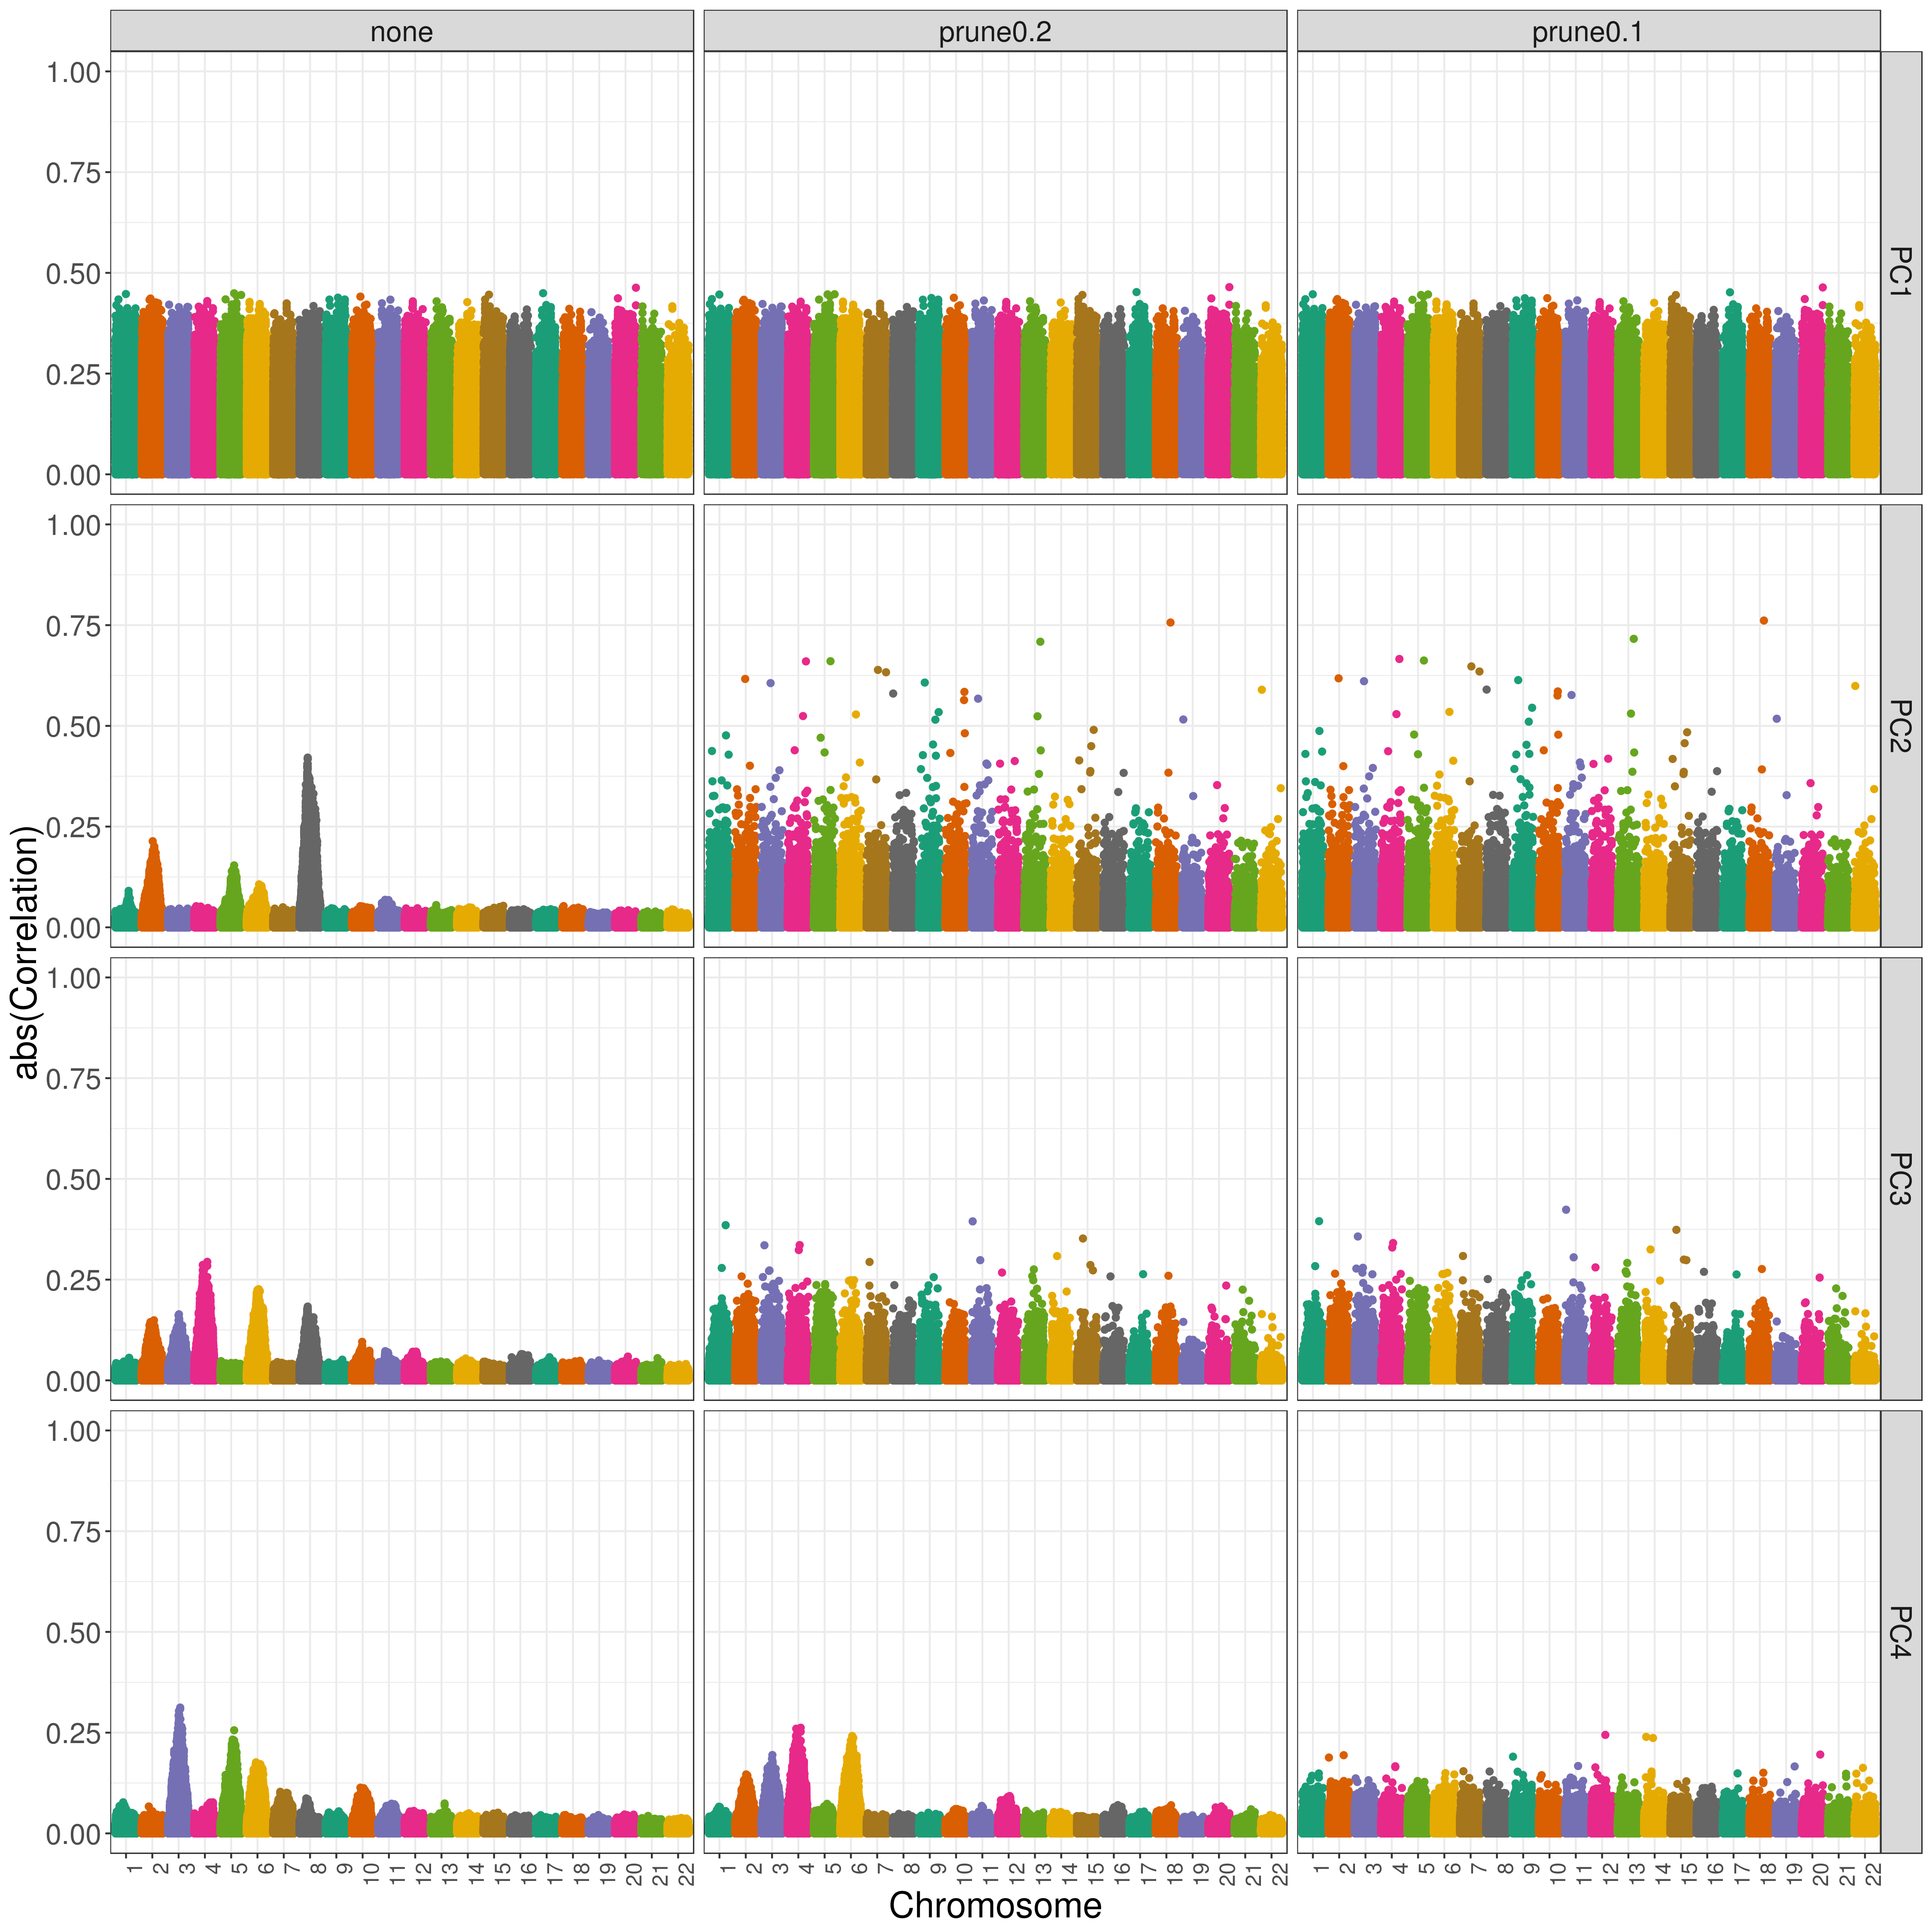
\includegraphics[width=\textwidth]{figs/pc_geno_corr/pc_geno_corr_compare_prune}
\caption{Correlation between PCs and genotypes in WHI SHARe African Americans using different LD pruning thresholds. Each panel plots the absolute value of the correlation between principal components and genotypes (on the y-axis) versus the position along the genome (x-axis).  Panels are organized vertically according to which PC is being investigated (1, 2, 3, 4) and horizontally according to what $r^2$ threshold was used when running LD pruning prior to PCA (\textit{none}: no LD pruning, \textit{prune0.2}: LD pruning with an $r^2$ threshold of 0.2 and window size of 0.5 Mb, and \textit{prune0.1}: LD pruning with an $r^2$ threshold of 0.1 and window size of 0.5 Mb).}
\label{fig:corr-compare-prune}
\end{figure}

\begin{figure}[h]
\center
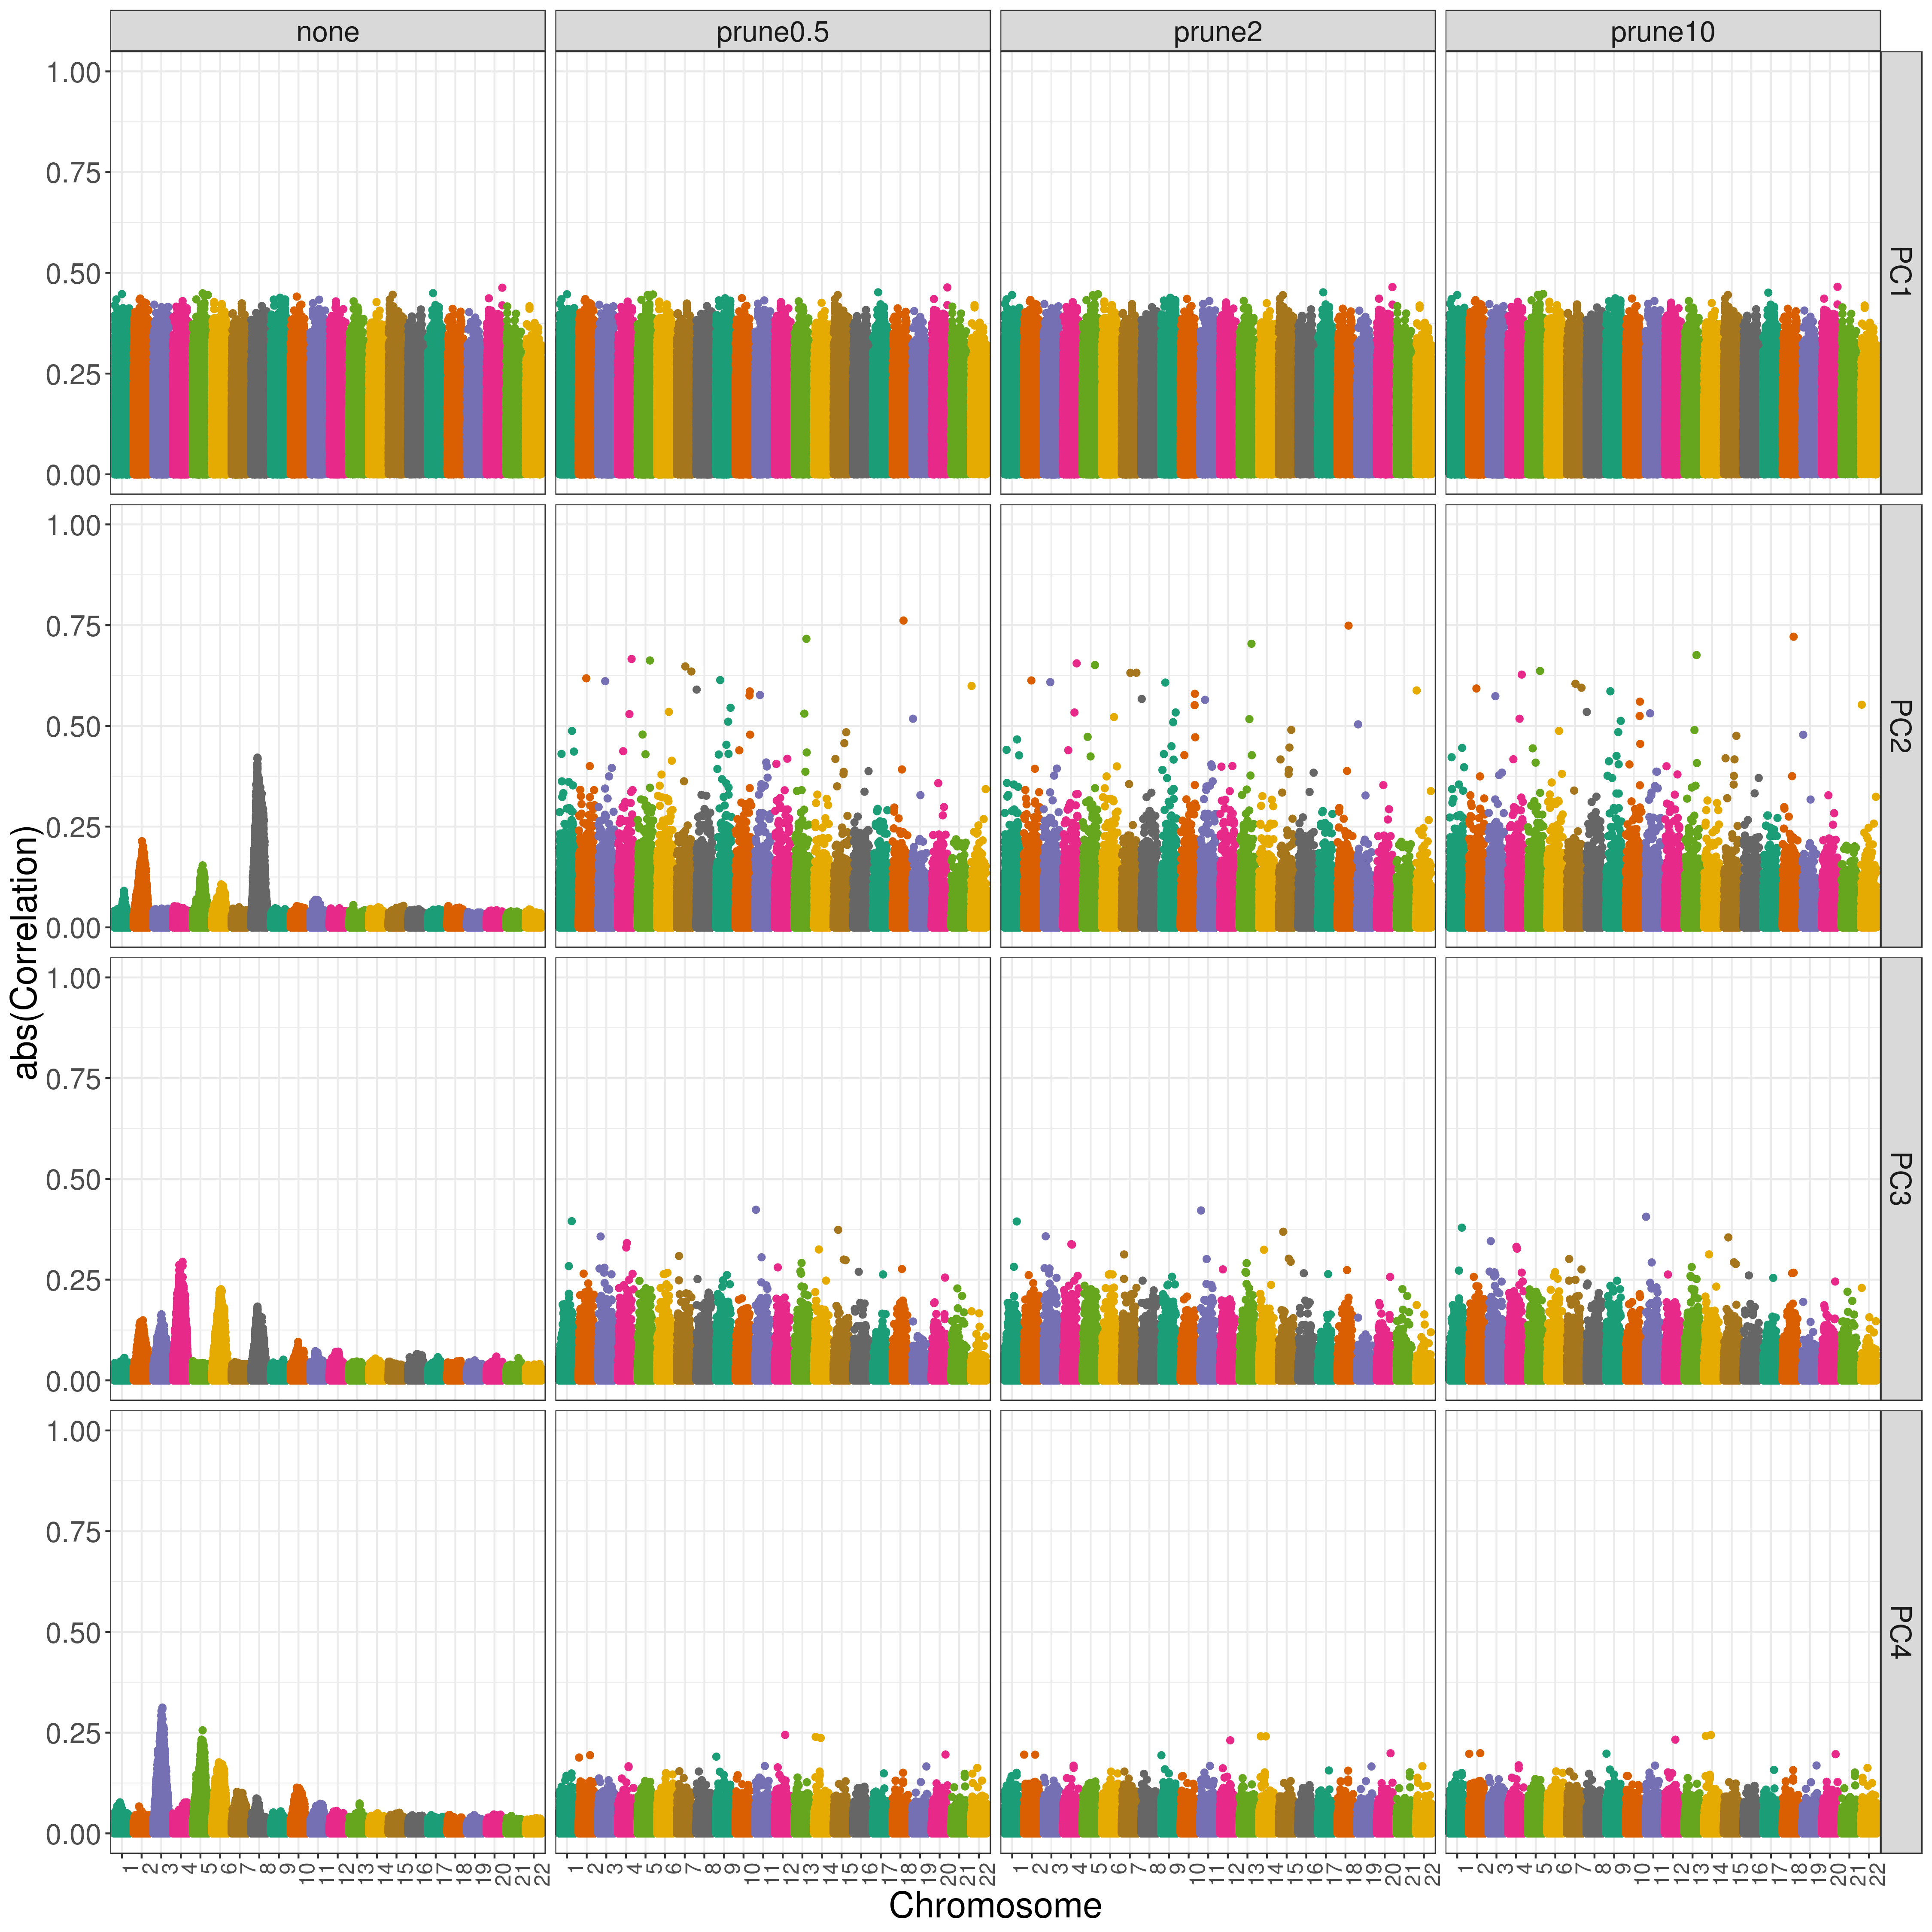
\includegraphics[width=\textwidth]{figs/pc_geno_corr/pc_geno_corr_compare_window}
\caption{Correlation between PCs and genotypes in WHI SHARe African Americans using different LD pruning window sizes. Each panel plots the absolute value of the correlation between principal components and genotypes (on the y-axis) versus the position along the genome (x-axis).  Panels are organized vertically according to which PC is being investigated (1, 2, 3, 4) and horizontally according to what window size was used when running LD pruning prior to PCA (\textit{none}: no LD pruning, \textit{prune0.5}: LD pruning with an $r^2$ threshold of 0.1 and window size of 0.5 Mb, \textit{prune2}: LD pruning with an $r^2$ threshold of 0.1 and window size of 2 Mb, and \textit{prune10}: LD pruning with an $r^2$ threshold of 0.1 and window size of 10 Mb).}
\label{fig:corr-compare-window}
\end{figure}

\begin{figure}[h]
\center
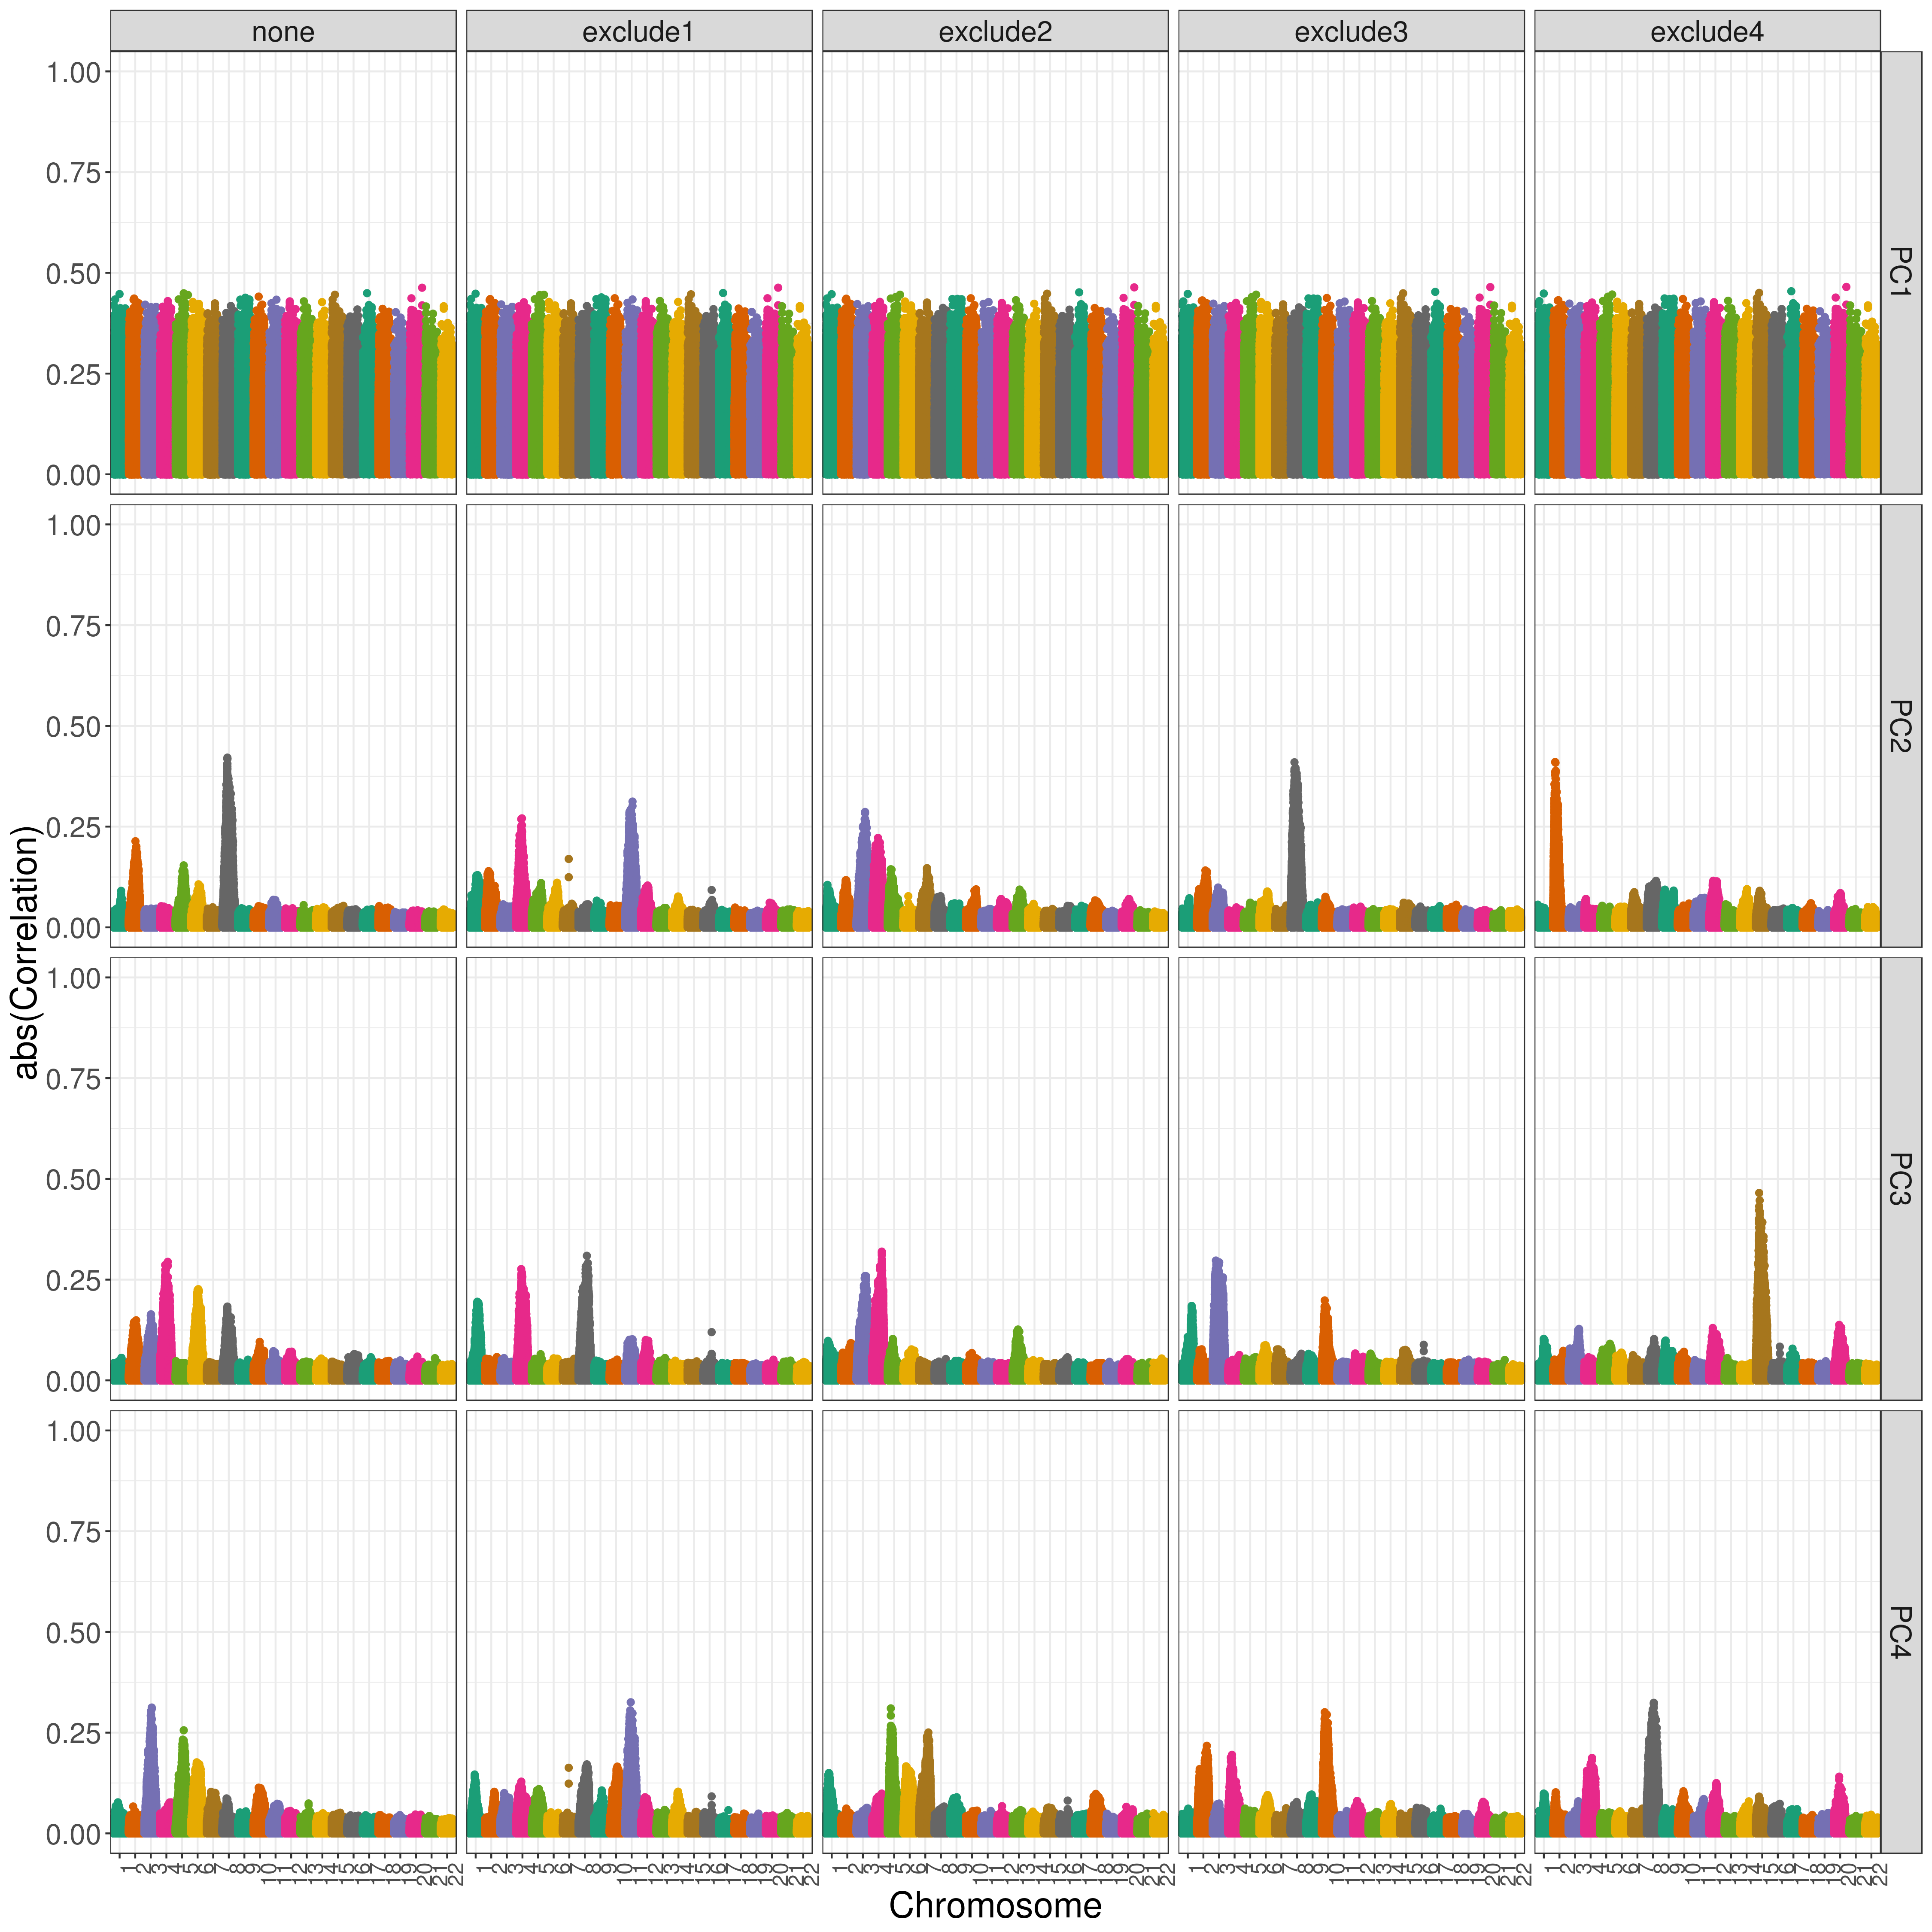
\includegraphics[width=\textwidth]{figs/pc_geno_corr/pc_geno_corr_compare_exclude}
\caption{Correlation between PCs and genotypes in WHI SHARe African Americans after multiple rounds of data-based exclusions. Each panel plots the absolute value of the correlation between principal components and genotypes (on the y-axis) versus the position along the genome (x-axis).  Panels are organized vertically according to which PC is being investigated (1, 2, 3, 4) and horizontally according to the number of iterations of our procedure for excluding regions highly correlated with PCs that were implemented prior to PCA (\textit{none}: no exclusions, \textit{exclude1}: one round of exclusions, \textit{exclude2}: two rounds of exclusions, etc.).}
\label{fig:corr-compare-exclude}
\end{figure}

\begin{figure}[h]
\center
\includegraphics[width=0.8\textwidth]{figs/COPD/EUR_prune_FALSE_1_0_0.01_snprelate_load_1}
\caption{SNP loadings for naively generated PCs in COPDGene European Americans. Each panel plots the principal component loading (y-axis) versus the position along the genome (x-axis) for each variant. Panels are organized vertically according to which PC is being investigated (1, 2, 3, 4). Unlike in admixed populations, we see a single peak on chromosome 11.}
\label{fig:corr-Eur}
\end{figure}

\begin{figure}[h]
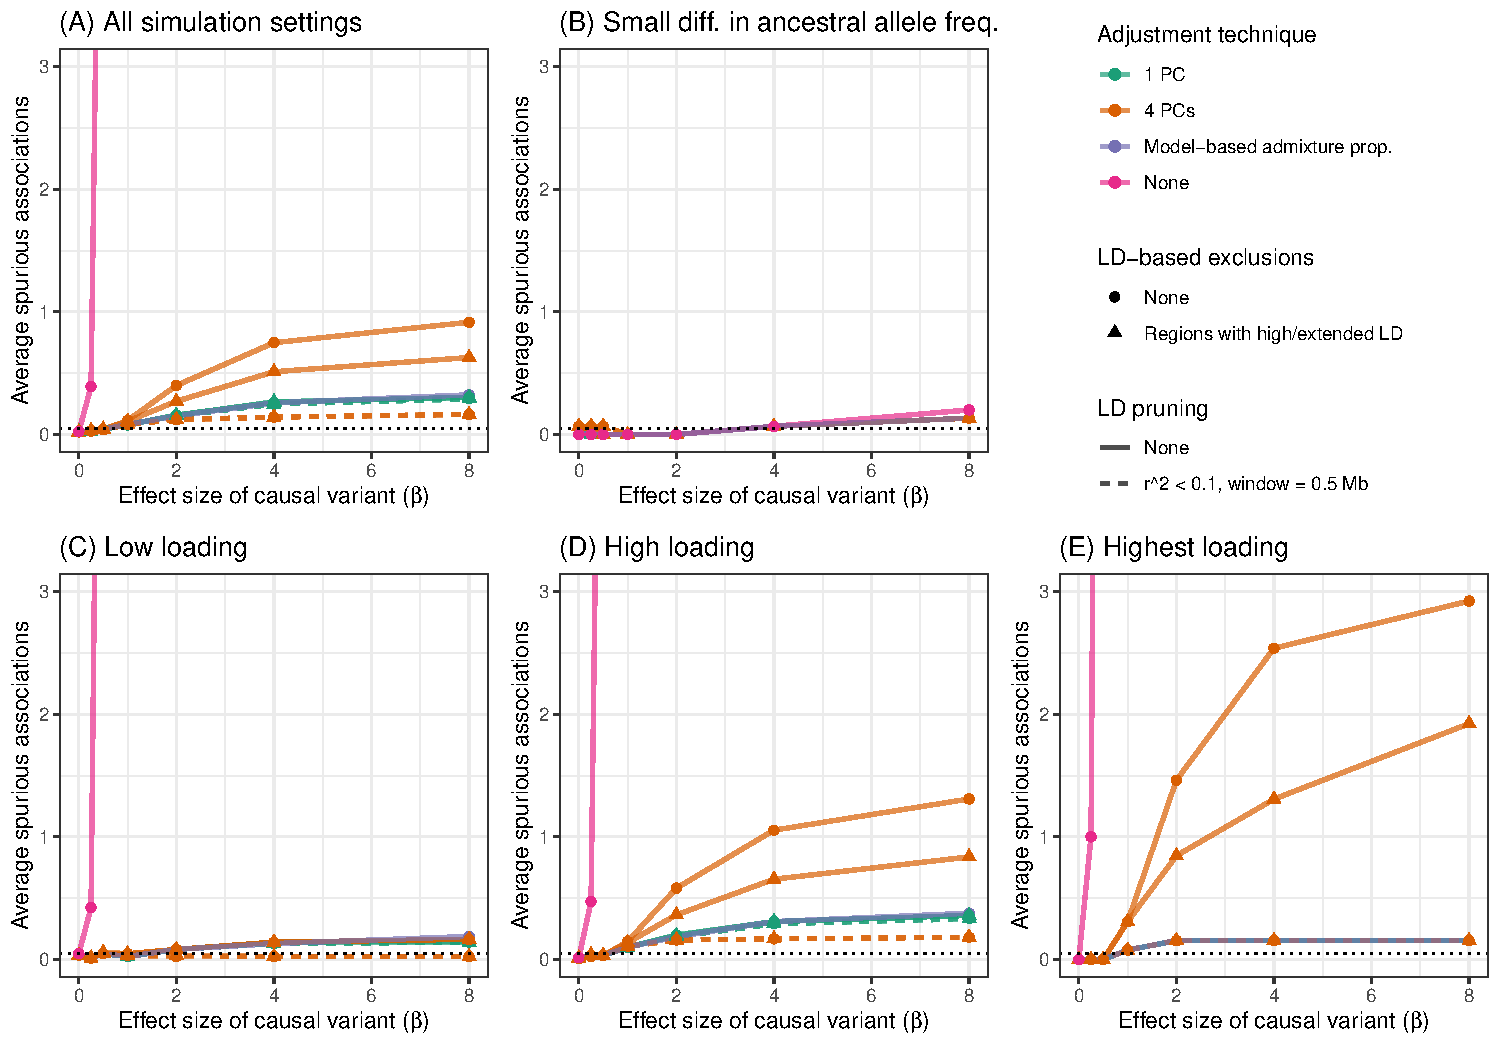
\includegraphics[width=\textwidth]{figs/spurious_counts/gwas/supplement_spurious_allbeta}
\caption{Comparison of the number of spurious associations in genome-wide association studies in WHI SHARe African Americans using different approaches to adjust for ancestral heterogeneity. Panels display the average number of spurious associations that were observed across (A) all simulation settings, or across the subset of simulation settings in which the causal variant has (B) a small difference in ancestral allele frequencies, (C) low SNP loadings for each of the first four PCs, (D) a high SNP loading for at least one of the first four PCs, or (D) the highest SNP loading on its chromosome for one of the first four PCs. Within each panel, we compare the number of spurious associations when GWAS models adjust for model-based admixture proportions, 1 PC (with or without LD pruning and/or Table \ref{tab:highLD} exclusions), or 4 PCs (with or without LD pruning and/or Table \ref{tab:highLD} exclusions). Results shown here are for simulated traits with a single causal variant, with effect size ($\beta$) ranging from 0 to 8.}
\label{fig:spurious-all-beta}
\end{figure}


\section*{Declaration of Interests}

% We ask that you and all authors disclose any personal financial interests (examples include stocks or shares in companies with interests related to the submitted work or consulting fees from companies that could have interests related to the work), professional affiliations, advisory positions, board memberships, or patent holdings that are related to the subject matter of the contribution. As a guideline, you need to declare an interest for (1) any affiliation associated with a payment or financial benefit exceeding $10,000 p.a. or 5% ownership of a company or (2) research funding by a company with related interests. You do not need to disclose diversified mutual funds, 401ks, or investment trusts.
% https://www.cell.com/declaration-of-interests

The authors declare no competing interests.


\section*{Acknowledgments}

% contributions from nonauthors
% list funding sources
% add any necessary data-related acknowledgments

K.E.G. was supported in part by the National Science Foundation Graduate Research Fellowship Program under grant no. DGE-1256082. Any opinions, findings, and conclusions or recommendations expressed in this material are those of the author(s) and do not necessarily reflect the views of the National Science Foundation.



\section*{Web Resources}

%list and provide URL for any web-based resources (e.g., datbase, online computer programs, etc.)
%For all computer programs, please provide a URL for the website at which the computer program described in the manuscript will be made publicly available.

\edit{GitHub Repository: lists of regions to exclude, code for LD pruning, excluding, and plotting loadings}


\section*{Data and Code Availability}

%statement describing the availability of new datasets and/or code associated with the paper.
%includes any conditions for access of datasets and/or code not publicly available.
%also include any accession numbers, DOIs or unique identifiers, or web links to deposited datasets

%%examples
%The [datasets/code] generated during this study are available at [name of repository] [accession code/web link].
%The published article includes all [datasets/code] generated or analyzed during this study.
%This study did not generate/analyze [datasets/code].
%There are restrictions to the availability of [dataset/code] due to [reason for restrictions].
%Original/source data for [figures/datatype] in the paper is available [e.g., Mendeley Data DOI].
%The [datasets/code] supporting the current study have not been deposited in a public repository because [reason data are not public] but are available from the corresponding author on request.

\newpage
\section*{References}

%include only articles that are published.
%"et al." should be used only after 10 authors.
%Please use the following styles for references:

%%Article in a periodical
%1. Leach, N.T., Sun, Y.,Michaud, S., Zheng, Y., Ligon, K.L., Ligon, A.H., Sander, T., Korf, B.R., Lu, W., Harris, D.J., et al. (2007). Disruption of diacylglycerol kinase delta (DGKD) associated with seizures in humans and mice. Am. J. Hum. Genet. 80, 792–799.

%%Article in a book
%2. King, S.M. (2003). Dynein motors: Structure, mechanochemistry and regulation. In Molecular Motors, M. Schliwa, ed. (Wiley-VCH Verlag GmbH), pp. 45–78.

%%Entire book
%3. Cowan, W.M., Jessell, T.M., and Zipursky, S.L. (1997). Molecular and Cellular Approaches to Neural Development (Oxford University Press).

%%Online reference
%4. Rothwarf, D.M., and Karin, M. (1999). The NF-kB pathway: a paradigm in information transfer from membrane to nucleus. Science’s STKE, http://www.stke.org/cgi/content/full/OC_sigtrans;1999/5/rel.

%%Computer program
%5. Hubbard, S.J. and Thornton, J.M. (1993). NACCESS computer program (Department of Biochemistry and Molecular Biology, University College London).
% Software may also be cited in text; for an in-text citation, include the name of the manufacturer in parentheses.

%%Dissertation/Thesis
%6. Smith, J.P. (1985). DNA sequences. PhD thesis (Massachusetts Institute of Technology).

%The current AJHG reference format for Endnote users can be downloaded from http://www.endnote.com/support/enstyles.asp
%The current AJHG reference format for RefMan users can be downloaded from http://www.refman.com/support/rmstyles.asp

%%In-Text Citations
%Unpublished data, abstracts, and personal communications may be cited within the text only. Submitted articles that have not yet been accepted should be cited as data not shown, unpublished data, or a personal communication.
%Unpublished data may refer only to work from an author of the manuscript being submitted.
%A personal communication should be documented by a letter of permission (this may be in the form of an e-mail communication, letter, or other appropriate form of permission).
%Please use the following style for such citations:

%%Unpublished data 
%(M.A., unpublished data)

%%Abstract
%(M. Adams et al., 1997, Soc. Neurosci., abstract)

%%Personal communication
%(M. Adams, personal communication) 

\bibliographystyle{ajhg}
\bibliography{spurious}


\newpage
\section*{Figure Titles and Legends}

% brief title describing entire figure without citing specific panels
% subsequent description of each panel

% numbered consecutively with whole numbers (e.g., Figure 1, Figure 2, etc. rather than Figure 1a, Figure 1b, etc.)

% figures may not exceed one page

% figure titles may not contain parenthetical information, reference citations, or footnotes

% all reference citations within a figure must also be included in the figure legend

%For any figures presenting pooled data, the measures should be defined in the figure legends (for example, data are represented as the mean ± SEM).

%%https://www.cell.com/figureguidelines


\section*{Tables}

%Include tables in the submitted manuscript after the figure titles and legends. Tables should not be saved as figures, i.e., as .jpg or .tif files. All tables intended for print should be incorporated into the end of the manuscript Word file. Tables should not be uploaded individually.

%When creating a table, please use the Microsoft Word table function, and please do not place an Excel table into a Word document. Tables not created with the Microsoft Word table function will be sent back for revision. Do not submit a table in PDF format.

%Word tables should not be tab or space delineatedand and should not include colored text or shading, but embedded graphics with color are OK.

%Do not use paragraph returns to separate data within a cell.

%Tables should include a title, and footnotes and/or legends should be concise. 

%Table titles may not contain parenthetical information, reference citations, or footnote citations.

%Use superscripted lowercase letters (beginning with “a”) for footnotes in tables. Do not use numbers or symbols.

%Tables must be numbered as Table 1, Table 2, Table 3, etc., rather than as Table 1a, Table 1b, Table 1c, etc.

%If italic font is used within a table to indicate some feature of the data, an explanation of its meaning must be given in the table legend. Bold text may not be used in tables.

%If a referenced paper or study is mentioned within a table, it must be included in the References list and must be followed by its appropriate citation number (e.g., “Author et al.1”) within the table.

%All abbreviations within a table must be defined in the table legend or footnotes.

\end{document}